% to choose your degree
% please un-comment just one of the following
\documentclass[bsc,twoside,singlespacing,parskip,logo,notimes,normalheadings]{infthesis}
% for BSc, BEng etc.

\usepackage[super]{natbib}
\setcitestyle{square}
\usepackage[toc]{appendix}

\usepackage[acronym,section,numberedsection=autolabel]{glossaries}

\makeglossaries

%% Basics
\newglossaryentry{controlflowgraph}
{
        name=control-flow graph,
        description={A graph representing the possible execution paths
        in a program. Nodes represent instructions, edges represent
        possible jumps between said instructions}
}

\newglossaryentry{dataflowanalysis}
{
        name=data-flow analysis,
        description={A technique for gathering information at various
          points in a \gls{controlflowgraph}}
}
 
\newglossaryentry{dataflow}
{
        name=data-flow,
        description={A system of equations and conditions which
          constitute a data-flow problem, that is, a problem which may
          be solved through data-flow analysis}
}

\newglossaryentry{direction}
{
        name=direction,
        description={The direction in which data flows in a
          \gls{dataflow} problem. Either forward (from the entry point
          of the \gls{cfg} to the exit point) or backward (the opposite)}
}

\newglossaryentry{localinformation}
{
        name=local information,
        description={Information specific to a given node in the CFG, e.g.
          in \gls{reachingdefinition}s DefGen is the set of definitions
          which a given node generates.}
}

\newglossaryentry{bitvector}
{
        name=bit-vector \gls{dataflow},
        description={\Gls{dataflow}s in which
          values come as single items, and are either included or
          excluded in each set. Such \gls{dataflow}s may be
          represented by a vector of bits, each bit representing a
          value and a 0 or 1 indicating the presence or absence of
          that value in the set.}
}

\newglossaryentry{tuplevalued}
{
        name=tuple-valued \gls{dataflow},
        description={\Gls{dataflow}s in which the values
          come in tuples; for example, in constant propagation each
          variable is paired with a value indicating whether it holds
          a constant.}
}

\newglossaryentry{dataflowequations}
{
        name=data-flow equations,
        description={A system of equations which determine how data
          flows through a \gls{cfg}}
}

\newglossaryentry{transfer}
{
        name=transfer,
        description={An equation (or set of equations) which
          determines how data flows {\em through} a node in a \gls{cfg}}
}

\newglossaryentry{meet}
{
        name=meet,
        description={An equation (or set of equations) which
          determines how data flows {\em between} nodes in a \gls{cfg}}
}

%%Graph Theory

\newglossaryentry{region}
{
        name=region,
        description={A set of nodes in a graph which includes a {\em header} node which \gls{dominate}s all other nodes in the region\cite[p. 669]{dragonbook}}
}

\newglossaryentry{dominate}
{
        name=dominate,
        description={In a \gls{cfg} a node $n_i$ is said to dominate a node $n_j$ if every path from $n_0$ (the entry node) to $n_j$ must go through $n_i$\cite[p. 478]{eac}}
}

%%Generic Frameworks 
\newglossaryentry{hassediagram}
{
        name=Hasse diagram,
        description={A diagram used to represent partially ordered
          sets. Nodes represent elements of the sets, edges represent
          an ordering between a pair of elements}
}

\newglossaryentry{meetsemilattice}
{
        name=meet semi-lattice,
        description={A partially ordered set in which there exists a
          greatest lower bound (or meet) for any non-empty, finite subset}
}

\newglossaryentry{meetoperator}
{
        name=meet operator,
        description={An operator which defines how the meet of two
          sets is obtained, such as $\cup$, $\cap$ or another operator
        entirely}
}

\newglossaryentry{domain}
{
        name=domain,
        description={The domain of values considered in a
          \gls{dataflow} problem, e.g. definitions or expressions}
}

\newglossaryentry{boundary}
{
        name=boundary,
        description={The initial value at the starting point of an
          analysis, i.e. $\text{In}(ENTRY)$ or $\text{Out}(EXIT)$}
}

\newglossaryentry{fixedpoint}
{
        name=fixed-point,
        description={A computation in which the required process is
          repeated until the state stops changing}
}


%% Types of Analysis
\newglossaryentry{reachingdefinition}
{
        name=reaching definition,
        description={A definition of a variable {\em reaches} a block if there exists at least one path from its definition to the block along which it is not overwritten}
}

\newglossaryentry{livenessanalysis}
{
        name=liveness analysis,
        description={A variable is {\em live} if its current value will be used later in the program's execution}
}

\newglossaryentry{availableexpression}
{
        name=available expression,
        description={An expression is {\em available} if it has been computed along all paths leading to the current node}
}

%% Parsing

\newglossaryentry{contextfreegrammar}
{
        name=context-free grammar,
        description={A context-free grammar describes a formal language using rules of the form $A \rightarrow \alpha$, in which $A$ is a single non-terminal symbol and $\alpha$ is a series of terminal or non-terminal symbols. The grammar is ``context-free'' in that its rules may be applied regardless of the context of the non-terminal $A$\cite{wikipedia:contextfreegrammar}}
}

%% Web Applications


\newglossaryentry{singlepageapp}
{
        name=single page app,
        description={a web application in which the page is only loaded once, after which
          JavaScript is used to update the content and asynchronous calls are
          used to request more data.}
}

%% Evaluation
 
\newglossaryentry{likertscale}
{
        name=Likert scale,
        description={A method of gauging opinion on a topic,
consisting of a collection of Likert items. Each Likert item contains
a statement followed by an odd number of responses, containing an
equal number of positive and negative responses balanced such that the
difference between responses is uniform. An example Likert item is the
oft-used Strongly Agree / Strongly Disagree scale, which may be
weighted from from 1-5. The Likert scale is the sum of weights of
responses to Likert items}
}


%% Acronyms
\newacronym{cfg}{CFG}{control-flow graph}
\newacronym{ui}{UI}{user interface}
\newacronym{ux}{UX}{user experience}
\newacronym{json}{JSON}{JavaScript Object Notation}
\glsunset{json}
\newacronym{drf}{DRF}{Django REST Framework}
\newacronym{dry}{DRY}{Don't Repeat Yourself}
\newacronym{cdn}{CDN}{content delivery network}
\newacronym{peg}{PEG}{Parsing Expression Grammar}
\newacronym{iloc}{ILOC}{Intermediate Language for Optimising Compilers}
\glsunset{iloc}
\newacronym{ast}{AST}{abstract syntax tree}
\newacronym{api}{API}{application programming interface}
\glsunset{api}
\newacronym{es6}{ES6}{ECMAScript 6}
\newacronym{copt}{COPT}{Compiler Optimisations}

%% Text
\usepackage{lipsum}
\usepackage{color}
\usepackage[dvipsnames]{xcolor}
\usepackage[hyphens]{url}
\renewcommand{\labelitemii}{$\circ$}

%% Math
\usepackage{amsmath}

%% Figures
\usepackage[section]{placeins}
\usepackage{tabularx}
%TC:ignore
\newcolumntype{C}{>{\centering\arraybackslash}X} % center column
\newcolumntype{T}[1]{>{\arraybackslash$\tt}{#1}<{$}} % math column
\newcolumntype{M}[1]{>{\arraybackslash$}{#1}<{$}} % math column
%TC:endignore
\usepackage{caption}
\captionsetup{%
  figurename=Fig.,
  tablename=Table
}
\usepackage{capt-of}
\usepackage{wrapfig}
\usepackage[bottom]{footmisc}
\usepackage[absolute,overlay]{textpos}
  \setlength{\TPHorizModule}{1mm}
  \setlength{\TPVertModule}{1mm}

\usepackage{listings}

\lstdefinelanguage{JavaScript}{
  keywords={typeof, new, true, false, catch, function, return, null, catch, switch, var, if, in, while, do, else, case, break},
  keywordstyle=\color{darkgray}\bfseries,
  ndkeywords={class, export, boolean, throw, implements, import, this},
  ndkeywordstyle=\color{darkgray}\bfseries,
  identifierstyle=\color{black},
  sensitive=false,
  comment=[l]{//},
  morecomment=[s]{/*}{*/},
  commentstyle=\color{Gray}\ttfamily,
  stringstyle=\color{Gray}\ttfamily,
  morestring=[b]',
  morestring=[b]"
}

\lstdefinelanguage{ILOC}{
  keywords={addI, cbr_LE, comp, storeAO,},
  keywordstyle=\color{darkgray}\bfseries,
  ndkeywords={cc},
  ndkeywordstyle=\color{darkgray}\bfseries,
  identifierstyle=\color{black},
  sensitive=false,
  comment=[l]{//},
  morecomment=[s]{/*}{*/},
  commentstyle=\color{darkgray}\ttfamily,
  stringstyle=\color{Gray}\ttfamily,
  morestring=[b]',
  morestring=[b]"
}


\lstset{
   extendedchars=true,
   basicstyle=\footnotesize\ttfamily,
   showstringspaces=false,
   showspaces=false,
   keywordstyle=\color{black}\bfseries,
   ndkeywordstyle=\color{black}\bfseries,
   identifierstyle=\color{black},
   numbers=left,
   numberstyle=\scriptsize,
   tabsize=2,
   breaklines=true,
   showtabs=false,
   xleftmargin=.04\textwidth,
}


%% Algorithm listings
\newcounter{nalg}[chapter] % defines algorithm counter for chapter-level
\newcounter{oldlstlisting}[chapter] % defines algorithm counter for chapter-level
\renewcommand{\thenalg}{\thechapter .\arabic{lstlisting}} %defines appearance of the algorithm counter
\DeclareCaptionLabelFormat{algocaption}{Algorithm \thenalg} % defines a new caption label as Algorithm x.y

\lstnewenvironment{algorithm}[1][] %defines the algorithm listing environment
{   
    \setcounter{oldlstlisting}{\value{lstlisting}}
    \setcounter{lstlisting}{\value{nalg}}
    \refstepcounter{nalg} %increments algorithm number
    \captionsetup{labelformat=algocaption,labelsep=colon} %defines the caption setup for: it ises label format as the declared caption label above and makes label and caption text to be separated by a ':'
    \lstset{ %this is the stype
        numbers=left,
        numberstyle=\scriptsize,
        basicstyle=\footnotesize,
        keywordstyle=\color{black}\bfseries,
        keywords={,input, output, return, datatype, function, in, if,
          else, foreach, while, begin, end, for, each, has, is, not, true, false, } %add the keywords you want, or load a language as Rubens explains in his comment above.
        ndkeywords{this,},
        ndkeywordstyle=\color{black}\bfseries,
        numbers=left,
        comment=[l]{//},
        commentstyle=\color{Gray},
        xleftmargin=.04\textwidth,
        tabsize=4,
        #1 % this is to add specific settings to an usage of this environment (for instnce, the caption and referable label)
    }
}
{\setcounter{lstlisting}{\value{oldlstlisting}}}

%% Graphs
\usepackage{tikz}
\usetikzlibrary{arrows.meta,decorations.markings,positioning,calc}

%% Tikz Styles
\tikzstyle{tree} = [rectangle, draw, text centered, rounded corners, minimum width=4mm, minimum height=6mm, below right]
\tikzstyle{atom} = [rectangle, draw, text centered, minimum width=6mm, minimum height=6mm, font=\tt\small]
\tikzstyle{block} = [rectangle, draw, text width=6em, text centered, rounded corners, minimum height=1em]
\tikzstyle{set} = [rectangle, text width=6em, text centered, rounded corners, minimum height=1em]
\tikzset{vertex/.style = {shape=circle,draw,minimum size=1.5em}}
\tikzset{edge/.style = {
    >=Stealth,
    -{>[scale=0.8]},
  }
}

\newcommand{\cfgpoint}[1][]{%
  \draw[magenta, fill=magenta!90] (#1) circle (0.5mm);
}

%% Superscript natbib citations
\makeatletter
\renewcommand\NAT@citesuper[3]{\ifNAT@swa
\if*#2*\else#2\NAT@spacechar\fi
\unskip\kern\p@\textsuperscript{\NAT@@open#1\if*#3*\else,\NAT@spacechar#3\fi\NAT@@close}%
   \else #1\fi\endgroup}
\makeatother

\begin{document}

\pagenumbering{roman}

\title{An Interactive Learning Platform for Compiler Data-Flow Analysis}

\author{Ayrton Massey}

% to choose your course
% please un-comment just one of the following
%\course{Artificial Intelligence and Computer Science}
%\course{Artificial Intelligence and Software Engineering}
%\course{Artificial Intelligence and Mathematics}
%\course{Artificial Intelligence and Psychology }   
%\course{Artificial Intelligence with Psychology }   
%\course{Linguistics and Artificial Intelligence}    
\course{Computer Science}
%\course{Software Engineering}
%\course{Computer Science and Electronics}    
%\course{Electronics and Software Engineering}    
%\course{Computer Science and Management Science}    
%\course{Computer Science and Mathematics}
%\course{Computer Science and Physics}  
%\course{Computer Science and Statistics}    

% to choose your report type
% please un-comment just one of the following
%\project{Undergraduate Dissertation} % CS&E, E&SE, AI&L
%\project{Undergraduate Thesis} % AI%Psy
\project{4th Year Project Report}

\date{\today}

\abstract{ \setcounter{page}{1} Data-flow analysis is one of the
  cornerstones of modern compiler optimisation. A thorough
  understanding of the processes involved is essential to further
  exploration of the subject. A tool which allows exploration of
  \gls{dataflowanalysis} in an interactive environment would prove
  invaluable to students encountering the topic for the first time.

  This report describes the design and implementation of an
  interactive system to simulate and visualise forms of data-flow
  analysis on simple assembly-like programs. The system is evaluated
  by in terms of user experience and the achievement of learning
  outcomes, through self-assessment and by examining usage data
  collected during the evaluation period.

  %TODO: Outcome
  The software proved (successful/unsuccessful) in providing a tool
  for increasing the learning capacity of the subjects.
}

\maketitle

\section*{Acknowledgements}
%TODO: Acknowledgements
Acknowledgements go here.

\tableofcontents

%%%%%%%%%%%%%%%%%%%%%%%%%%%%%%%%%%%%%%%
\chapter{Introduction}
\pagenumbering{arabic}

This chapter gives a short introduction to the topic of data-flow
analysis, describes motivations and desired outcomes for the project
and provides a brief summary of contributions.


    \section{Data-Flow Analysis}
    \Gls{dataflowanalysis} is a tool for analysing the flow of data
    through a program at various points in its execution. Analysis is
    performed over a \gls{controlflowgraph}, computing the properties
    of values flowing {\em in} and {\em out} of each node. Many forms
    of data-flow analysis exist to compute various properties, for
    example {\em \gls{livenessanalysis}} identifies variables which
    will be used in future instructions and {\em
      \gls{availableexpression}s} identifies those expressions whose
    value has been previously computed at some point in the
    \gls{controlflowgraph}.
    
    This analysis is used to inform optimisations which can be
    performed on a given program. Using the example of {\em
      \gls{livenessanalysis}}, the values computed can be used to
    optimise register allocation: a variable which is not live at a
    given point does not need to be allocated to a register, enabling
    more efficient use of available resources.
    
    Data-flow analysis is not only useful in compiler
    optimisation. The information gathered can be used in other ways,
    such as identifying unsafe operations in PHP web
    applications\cite{TaintedFlow} by monitoring
    sanitization\footnote{To {\em sanitize} a user input is to remove
      any potentially dangerous elements from said input; for example,
      if a user input string is to be inserted into the HTML of a
      webpage it could be sanitized by replacing instances of {\tt
        \textless} and {\tt \textgreater} with {\tt \&lt;} and {\tt
        \&gt;}, respectively. This would prevent that input being
      misinterpreted as HTML and thus avoid malicious scripts
      contained within that input from being executed.} of variables
    which have been assigned to user input.


    \section{Motivations}
    This project was inspired by the project's supervisor, Hugh
    Leather. The original concept was an online tutor for
    \gls{dataflowanalysis} which would allow users to simulate an
    analysis on simple programs. The user could vary parameters, such
    as the \gls{dataflow} in question or the order in which nodes are
    evaluated, and examine the resulting solution.
    
    As lecturer of the \gls{copt} course at the University
    of Edinburgh, Dr. Leather desired a system which could teach
    students the foundations of the course in a more interactive
    format than standard lectures. The system should be suitable for
    hosting on the course web page to make it accessible to all
    students.
    
    My personal interest in this project stemmed from a desire to use
    my practical skills to increase my capacity for understanding
    theoretical content. As noted in our early discussions, many
    students find it difficult and time consuming to read and
    understand material from the course textbook. Presenting this
    information in such a way that it could be easily digested by even
    a novice to Computer Science provided an exciting challenge.
    
    
    \section{Objectives}
    The main aim of this project was to create an interactive system
    to teach students the basic principles of \gls{dataflowanalysis}
    in compilers.
    
    This would take the form of a web application using visual
    components which could be combined in different ways, for example
    to present a series of tutorials on \gls{dataflowanalysis} or to
    provide a sandbox environment to explore. The content of the
    application would cover a range of topics from the basics of
    \gls{dataflowanalysis} to algorithms and frameworks for solving
    generic \gls{dataflow} problems.
    
    The application would be aimed at students of the \gls{copt}
    course and as such would be based on material from the course
    textbook {\em Engineering a Compiler, 2nd ed.}\cite{eac} by Keith
    D. Cooper and Linda Torczon. The application could then be
    extended to cover the topic in more depth using content from {\em
      Compilers: Principles, Techniques and Tools, 1st
      ed.}\cite{dragonbook} by Alfred V. Aho, Ravi Sethi and Jeffery
    D. Ullman.
    
    Users would be able to interact with the system by providing
    simple assembly-like programs, altering parameters of the analysis
    and stepping through a simulation. Elements of the simulation such
    as the current state and the \gls{controlflowgraph} of the program
    would be visualised on-screen and update as the simulation
    progressed. Each of these elements would be linked visually to
    show how the concepts relate.
    
    The application would be tested on real users. It would be
    evaluated in terms of user experience by analysing interactions
    with the system and conducting a user experience
    survey. Achievement of learning outcomes would be assessed by
    examining responses to questions built into the software and
    self-assessment by the user.
    
    \section{Summary of Contributions}
    The final version of the software is capable of the following:
    
    \begin{itemize}
    \item Simulation of pre-defined \gls{dataflow}s using generic
      framework models. (p. )%TODO: Which page?
    \item Simulation of user-defined programs using the
      \gls{iloc}\cite[appx.~A]{eac} language from {\em Engineering a
        Compiler}. (p. )%TODO: Which page?
    \item Simulation using the round-robin iterative algorithm (p.
      ) %TODO: Which page?
    \item User-controlled simulation allowing step-by-step, instant or
      automated playback.
    \item Visualisation of the following simulation elements:
      \begin{itemize}
      \item \Gls{controlflowgraph} (p. )%TODO: Which page?
      \item Simulator state incl. currently evaluated node,
        framework etc. (p. )%TODO: Which page?
      \item Table of results displaying data flowing in / out of each
        node.
      \item \Gls{hassediagram} of \gls{meetsemilattice} (p.
        ) %TODO: Which page?
      \end{itemize}
    \item Tutorials covering basics of the topic with interactive
      elements (p. )%TODO: Which page?
    \item Interactive test to assess achievement of learning outcomes
    \end{itemize}

    In addition, I have produced an API to record user interaction
    events modeled on the Google Analytics event tracking system
    (p. ). %TODO: Which page?

    Detailed explanations of the terminology mentioned above can be
    found in chapter \ref{chap:background}. A quick summary of terms
    can be found in the glossary in appendix \ref{appx:glossary}.


%%%%%%%%%%%%%%%%%%%%%%%%%%%%%%%%%%%%%%%
\chapter{Background}\label{chap:background}
This chapter briefly covers the necessary background information
required to understand this project, both to inform the reader and to
demonstrate understanding of the topic.

    \section{Introduction to Data-Flow Analysis}
    Data-flow analysis computes information about data flowing {\em
      in} and {\em out} of each node in a program's
    \gls{controlflowgraph}. Many types of analysis can be performed
    and the information gathered can be used to inform the decisions
    of optimising compilers. A brief list of analyses and their
    purposes can be found in appendix \ref{appx:analysistypes}.
    
        \subsection{Control-flow Graph}

        \begin{textblock}{80}(20,176)
            \begin{tikzpicture}[y=-1cm, remember picture]
              % vertices
              \node[block] (n1) at (2 , 0) {\tt a = X[i]};
              \node[block] (n2) at (2 , 1) {\tt b = Y[i]};
              \node[block] (n3) at (2 , 2) {\tt if a > b};
              \node[block] (n4) at (0 , 3) {\tt Z[i] = a};
              \node[block] (n5) at (4 , 3) {\tt Z[i] = b};
              \node[block] (n6) at (2 , 4) {\tt i++};
              \node[block] (n7) at (2 , 5.3) {\tt if i < Z.length};
              \node (n8) at (2 , 6.6) {$\cdots$};
              
              % edges
              \draw[edge] (n1)       to (n2);
              \draw[edge] (n2)       to (n3);
              \draw[edge] (n3.south) to (n4);
              \draw[edge] (n3.south) to (n5);
              \draw[edge] (n4) to (n6.north);
              \draw[edge] (n5) to (n6.north);
              \draw[edge] (n6) to (n7);
              \draw[edge] (n7) to (n8);
              \draw[edge] (n7.east) -| ++(2.5, 0) |- (2.5, -0.8) -| (n1.north);

              \cfgpoint[n3.south];
              \cfgpoint[n6.north];
              
            \end{tikzpicture}
            \captionsetup{width=8cm,justification=justified}
            \captionof{figure}{A control-flow graph.}
            \label{fig:cfgexample}
        \end{textblock}

        \hfill\begin{minipage}{\dimexpr\textwidth-6cm}

          A \gls{controlflowgraph} displays the possible execution
          paths for a given program. Each node in the graph represents
          an instruction or basic block, each edge represents an
          execution path leading from that instruction. A node can
          have multiple outward edges if it is a branching
          instruction. Branches may point backward in the
          control-flow. An example of a simple \gls{controlflowgraph}
          can be seen in fig. \ref{fig:cfgexample}.
          
          \vspace{0.26cm}

          A {\em point} in the \gls{controlflowgraph} refers to some
          point along the edges of the graph. In
          \gls{dataflowanalysis} we usually deal with sets of values
          at the {\em in} and {\em out} points of each node, i.e. the
          point where the {\em in-edges} meet and the {\em out-edges}
          originate, respectively (shown in
          \textcolor{magenta}{magenta} on the left).

        \end{minipage}

	\subsection{A Simple Example}\label{sec:simpleexample}
	An oft-used example of \gls{dataflowanalysis} is that of {\em
          \gls{reachingdefinition}s}, which we will demonstrate here
        due to its simplicity. \Gls{reachingdefinition}s computes the
        set of variable definitions which are are available at a given
        point. A definition is said to {\em reach} a point $p$ if
        there is no intermediate assignment to the same variable along
        the path from the definition of the variable to the point $p$.
        
        Let us take the example in fig. \ref{fig:cfgexample}. The first
        node defines the variable {\tt a}. We shall refer to this
        definition of {\tt a} as {\tt a\textsubscript{1}}. The
        definition of {\tt a} reaches each point in the
        \gls{controlflowgraph} as it is never re-defined. The
        definition {\tt c\textsubscript{1}}, however, does not reach
        the exit node as {\tt c} is re-defined by {\tt
          c\textsubscript{2}}. The graph in fig. \ref{fig:rdcfg} shows the
        set of reaching definitions at each point in the program. We
        have combined the {\em in} and {\em out} points to save space.
                
        Data-flows have {\em direction}. Reaching definitions is a
        {\em forward flow problem}; values flow from the entry node of
        the \gls{cfg} to the exit node.

        \begin{wrapfigure}[21]{i}{6.5cm}
          \centering
          \vspace{-5mm}
          \begin{tikzpicture}[y=-1cm]
            % vertices
       	    \node[set] (s0) at (3 , -1) {\tt \{\}};
            \node[block] (n1) at (0 , 0) {\tt a\textsubscript{1} = 1};
       	    \node[set] (s1) at (3 , 1) {\tt \{a\textsubscript{1}\}};
            \node[block] (n2) at (0 , 2) {\tt b\textsubscript{1} = a + 1};
            \node[set] (s2) at (3 , 3) {\tt \{a\textsubscript{1}, b\textsubscript{1}\}};
            \node[block] (n3) at (0 , 4) {\tt c\textsubscript{1} = a + b};
            \node[set] (s3) at (3 , 5) {\tt \{a\textsubscript{1}, b\textsubscript{1}, c\textsubscript{1}\}};
            \node[block] (n4) at (0 , 6) {\tt c\textsubscript{2} = 0};
            \node[set] (s4) at (3 , 7) {\tt \{a\textsubscript{1}, b\textsubscript{1}, c\textsubscript{2}\}};
            \node[block] (n5) at (0 , 8) {\tt return c};
       	    \node[set] (s5) at (3 , 9) {\tt \{a\textsubscript{1}, b\textsubscript{1}, c\textsubscript{2}\}};

            \node[above=0mm of n1.north west] (an1) {$n_1$};
            \node[above=0mm of n2.north west] (an2) {$n_2$};
            \node[above=0mm of n3.north west] (an3) {$n_3$};
            \node[above=0mm of n4.north west] (an4) {$n_4$};
            \node[above=0mm of n5.north west] (an5) {$n_5$};
            
            %edges
            \draw[edge] (n1) to (n2);
            \draw[edge] (n2) to (n3);
            \draw[edge] (n3) to (n4);
            \draw[edge] (n4) to (n5);

            \cfgpoint[n1.north]
            \cfgpoint[n1.south]
            \cfgpoint[n2.north]
            \cfgpoint[n2.south]
            \cfgpoint[n3.north]
            \cfgpoint[n3.south]
            \cfgpoint[n4.north]
            \cfgpoint[n4.south]
            \cfgpoint[n5.north]
            \cfgpoint[n5.south]
            
            %set lines
            \draw[edge, dotted] (s1.west) to [bend left] (n1.south);
	    \draw[edge, dotted] (s2.west) to [bend left] (n2.south);
	    \draw[edge, dotted] (s3.west) to [bend left] (n3.south);
	    \draw[edge, dotted] (s4.west) to [bend left] (n4.south);
	    \draw[edge, dotted] (s5.west) to [bend left] (n5.south);
            \draw[edge, dotted] (s0.west) to [bend right] (n1.north);
            \draw[edge, dotted] (s1.west) to [bend right] (n2.north);
	    \draw[edge, dotted] (s2.west) to [bend right] (n3.north);
	    \draw[edge, dotted] (s3.west) to [bend right] (n4.north);
	    \draw[edge, dotted] (s4.west) to [bend right] (n5.north);
            
          \end{tikzpicture}
          \captionsetup{justification=centering}
          \caption{A \gls{controlflowgraph}.}
          \label{fig:rdcfg}
        \end{wrapfigure}

        The values at each point are determined using {\em data-flow
          equations}. For example, the equations for reaching
        definitions (defined in terms of {\em in} and {\em out}) at a
        given node $n$ are:
        
        \vspace{-7mm}
        \begin{align*}
          \textnormal{In}(n)  & = \bigcup_{p \in preds} \textnormal{Out}(n) \\
          \textnormal{Out}(n) & = \textnormal{DefGen}(n) \cup (\textnormal{In}(n) \setminus \textnormal{DefKill}(n))
        \end{align*}
        
        The equations for $\text{In}(n)$ and $\text{Out}(n)$ are often
        referred to as {\em \gls{meet}} and {\em \gls{transfer}}
        functions. Other symbols such as $\text{DefGen}(n)$ and
        $\text{DefKill}(n)$ are referred to as \gls{localinformation},
        as they are constant values containing information about the
        current node. In a forward flow problem the meet function
        combines the {\em out} sets of a node's predecessors to form
        its {\em in} set. The \gls{transfer} function computes a
        node's {\em out} set from its {\em in} set and information
        obtained from the node itself, thereby {\em transferring}
        values through a node.

	\subsection{Lattices}\label{sec:background_lattices}
	Sets in a \gls{dataflow} problem have a partial order. This
        can be expressed using a structure known as a {\em
          \gls{meetsemilattice}}. A \gls{meetsemilattice} consists of
        a set of possible values $L$, the meet operator $\land$, and a
        {\em bottom element} $\bot$. The semi-lattice imposes an order
        on values in $L$ such that:
        
        \vspace{-1cm}
        %TODO: REFERENCE
        \begin{align*}
          a \geq b \;\text{if and only if}\; & a \land b = b \\
          a \ge  b \;\text{if and only if}\; & a \land b = b \;\text{and}\; a \neq b
        \end{align*}
        \vspace{-1cm}
        
        For the bottom element $\bot$, we have the following:
        
        \vspace{-1cm}
        %TODO: REFERENCE
        \begin{align*}
          \forall a \in L,\; & a \geq \bot \\
          \forall a \in L,\; & a \land \bot = \bot
        \end{align*}
        \vspace{-1cm}
        
        %TODO: REFERENCE
        The semi-lattice can be expressed using a {\em \gls{hassediagram}}, shown in fig. \ref{fig:meethasse}.

        \begin{figure}[h]
          \centering
          \begin{tikzpicture}[y=-1cm]            
            % vertices
       	    \node[set, label={[distance=1cm]0:$(\top)$}] (s1) at (2 , 0.0) {$\emptyset$};
	    \node[set] (s2) at (0 , 1.5) {\tt \{a\}};
            \node[set] (s3) at (2 , 1.5) {\tt \{b\}};
            \node[set] (s4) at (4 , 1.5) {\tt \{c\}};
	    \node[set] (s5) at (0 , 3.0) {\tt \{a, b\}};
	    \node[set] (s6) at (4 , 3.0) {\tt \{b, c\}};
            \node[set] (s7) at (2 , 3.0) {\tt \{a, c\}};
	    \node[set, label={[distance=1cm]0:$(\bot)$}] (s8) at (2 , 4.5) {\tt \{a, b, c\}};
            
            %set lines
            \draw[edge] (s1.south) -- (s2.north);
            \draw[edge] (s1.south) -- (s3.north);
            \draw[edge] (s1.south) -- (s4.north);
            
            \draw[edge] (s2.south) -- (s5.north);
            \draw[edge] (s2.south) -- (s7.north);
            \draw[edge] (s3.south) -- (s5.north);
            \draw[edge] (s3.south) -- (s6.north);
            \draw[edge] (s4.south) -- (s6.north);
            \draw[edge] (s4.south) -- (s7.north);
            
            \draw[edge] (s5.south) -- (s8.north);
            \draw[edge] (s6.south) -- (s8.north);
            \draw[edge] (s7.south) -- (s8.north);
            
          \end{tikzpicture}
          \captionsetup{justification=centering}
          \caption{A \gls{hassediagram} for the meet function $a \land b = a \cup b$.}
          \label{fig:meethasse}
        \end{figure}
        
        \subsection{Bit-Vector Data-Flows}
        
        The \gls{dataflow}s present in the system described in this
        project are commonly known as \gls{bitvector}s. In these
        problems values are single items, such as a variable or
        definition. A set of values can be represented as a vector of
        bits, each bit representing a particular value and a 0 or 1
        indicating the presence or absence of that value. The
        \gls{reachingdefinition}s example from the previous section is
        a \gls{bitvector} problem. Fig. \ref{fig:bitvector} shows how
        this can be applied to the example in
        \S\ref{sec:simpleexample}.

        \begin{figure}[!ht]
          \centering
          \begin{tabular}{M{r} M{c} T{r} T{c} T{c} T{c} T{c} T{l}}
                            &   &    & a_1 & b_1 & c_1 & c_2 &    \\
            \text{Out}(n_5) & = & \{ & 1   & 1   & 0   & 1   & \} \\
          \end{tabular}
          \caption{A bit-vector for the \gls{cfg} in fig. \ref{fig:rdcfg}}\label{fig:bitvector}
        \end{figure}

        % TODO: Reference
        \Gls{tuplevalued}s consider values as tuples instead of single
        items. One such example is constant propagation, in which
        variables are paired with one of three elements:
        $undef\;(\top)$, $nonconst\;(\bot)$ and $const$. A variable is
        initially paired with $undef$. When it is assigned a constant
        value, we assign it that particular value. If it is later
        assigned another value, we assign it $nonconst$. This can be
        expressed as the meet function, $\land$, seen in
        fig. \ref{fig:constmeet}. The values form the semi-lattice in
        fig. \ref{fig:consthasse}.

        \begin{figure}[h]
        \begin{align*}
        nonconst \land c     & = nonconst & \text{for any constant} \; c         \\
        c \land d            & = nonconst & \text{for any constants} \; c \neq d \\
        c \land undef        & = c        & \text{for any constant} \; c         \\
        nonconst \land undef & = nonconst &                                      \\
        x \land x            & = x        & \text{for any value} \; x
        \end{align*}
        \caption{Equations describing the constant propagation meet function.}
        \label{fig:constmeet}
        \end{figure}
        
        \begin{figure}[h]
          \centering
          \begin{tikzpicture}[y=-1cm]
            
            % vertices
       	    \node[set, label={[distance=1cm]0:$(\top)$}] (s1) at (3.5 , 0) {$undef$};
            \node[set] (s0) at (0, 1) {$\dots$};
	    \node[set] (s2) at (1 , 1) {$c_1$};
            \node[set] (s3) at (2 , 1) {$c_2$};
            \node[set] (s4) at (3 , 1) {$c_3$};
            \node[set] (s5) at (4 , 1) {$c_4$};
            \node[set] (s6) at (5 , 1) {$c_5$};
       	    \node[set] (s7) at (6, 1) {$c_6$};
            \node[set] (s9) at (7, 1) {$\dots$};
	    \node[set, label={[distance=1cm]0:$(\bot)$}] (s8) at (3.5 , 2) {$nonconst$};
            
            %set lines
            \draw[edge] (s1.south) -- (s2.north);
            \draw[edge] (s1.south) -- (s3.north);
            \draw[edge] (s1.south) -- (s4.north);
            \draw[edge] (s1.south) -- (s5.north);
            \draw[edge] (s1.south) -- (s6.north);
            \draw[edge] (s1.south) -- (s7.north);
            
            \draw[edge] (s2.south) -- (s8.north);
            \draw[edge] (s3.south) -- (s8.north);
            \draw[edge] (s4.south) -- (s8.north);
            \draw[edge] (s5.south) -- (s8.north);
            \draw[edge] (s6.south) -- (s8.north);
            \draw[edge] (s7.south) -- (s8.north);
            
          \end{tikzpicture}
          \caption{A \gls{hassediagram} for the meet function described in fig \ref{fig:constmeet}.}
          \label{fig:consthasse}
        \end{figure}
        
    \pagebreak
    
    \section{Algorithms for Analysis}
    There exist a number of algorithms for performing
    \gls{dataflowanalysis}. This section contains a brief overview of
    the methods proposed in the related reading \cite{eac}
    \cite{dragonbook}.

        \subsection{Round-Robin Iterative Algorithm}
        The simplest algorithm used to solve \gls{dataflow} problems
        is the round-robin iterative method. We consider each node of
        the \gls{cfg} in turn, calculating the In and Out sets using
        our \gls{dataflowequations}. This is a \gls{fixedpoint}
        computation: we iterate until our value sets stop changing
        between iterations. Algorithm \ref{algo:rd_iterative} shows
        the round-robin iterative method for solving
        \gls{reachingdefinition}s.

        \begin{figure}[h]
          \begin{algorithm}[caption={Iterative Round-Robin Method for Reaching Definitions}, label={algo:rd_iterative},escapeinside={||},mathescape=true]
for each (node |$n$| in the CFG)
    In(|$n$|) = |$\emptyset$|;

while (changes to any sets occur)
    for each (node |$n$| in the CFG)
        In(|$n$|)  = |$\cup$\textsubscript{predecessors $p$ of $n$}|Out(|$p$|);
        Out(|$n$|) = DefGen(|$n$|) $\cup$ (In|$(n)$| $\setminus$ DefKill(|$n$|));
          \end{algorithm}
        \end{figure}

        \subsection{Worklist Algorithm}
        The above solution holds value in its simplicity, but it is
        trivial to find a more efficient solution. A node's sets will
        only change if the Out sets of its predecessors change. Thus,
        we may use a worklist: starting with the initial node, we
        calculate the Out set for that node; if it changes we add the
        node's successors to the list. We continue this process until
        the worklist is empty. Algorithm \ref{algo:rd_worklist} shows
        the worklist method for solving \gls{reachingdefinition}s.

        \begin{figure}[h]
          \begin{algorithm}[caption={Worklist  Method for Reaching Definitions}, label={algo:rd_worklist},escapeinside={||},mathescape=true]
worklist = [ n|$_{0}$| ];

while (worklist is not empty)
    n = pop(worklist);
    In(|$n$|)  = |$\cup$\textsubscript{predecessors $p$ of $n$}|Out(|$p$|);
    Out(|$n$|) = DefGen(|$n$|) $\cup$ (In|$(n)$| $\setminus$ DefKill(|$n$|));
    if (Out(|$n$|) has changed) append n to worklist;
          \end{algorithm}
        \end{figure}

        \subsection{Structural Algorithm}
        A third algorithm takes an entirely different
        approach. Instead of iterating over each node, we perform a
        number of simple transformations on the graph in order to
        reduce it to a single \gls{region}. We then expand each node,
        calculating the In and Out sets of our reduced nodes as we
        expand them. A more detailed explanation of this concept may
        be found in the {\em Dragon Book}\cite[p. 673]{dragonbook}.

    \section{Data-Flow Frameworks}\label{sec:background-frameworks}

    It is possible to model \gls{dataflow} problems using a generic
    framework. This allows us to use the same algorithm for multiple
    problems by specifying the following constraints\cite[p. 680]{dragonbook}:

    \begin{itemize}
    \item The {\em \gls{domain}} of values on which to operate;
    \item The {\em \gls{direction}} in which data flows;
    \item A set of {\em \gls{dataflowequations}} including the {\em
        \gls{meetoperator}} $\land$ and the set of {\em
        \gls{transfer} functions} $F$\footnote{The function
        corresponding to a particular node/block $B$ is denoted $F_{B}$};
    \item The {\em \gls{boundary}} value $v_{BOUNDARY}$ specifying
      the value at the entry or exit to the \gls{cfg}; and
    \item The {\em initial value}, $\top$, at each point in the graph.
    \end{itemize}
    
        \subsection{Algorithm for General Frameworks}

        Algorithm \ref{algo:general}, adapted from the one in the {\em
          Dragon Book}\cite[p. 691]{dragonbook}, computes the value
        sets at each node using the elements of our general
        framework.

        \begin{algorithm}[caption={Data-Flow Analysis of General Frameworks}, label={algo:general},escapeinside={||},mathescape=true]
Meet|$_{BOUNDARY}$| = v|$_{BOUNDARY}$|;

for each (block |$B$| in the CFG)
    Meet|$_{B}$| = |$\top$|;

while (changes to any Transfer occur)
    for each (block |$B$| in the CFG)
        Meet|$_{B}$|     = |$\land$\textsubscript{priors $P$ of $B$}| Transfer|$_{P}$|;
        Transfer|$_{B}$| = |$F_{B}$|(In|$_{B}$|);
       \end{algorithm}

        Instead of referring to the value sets as In and Out as the
        {\em Dragon Book} does, we may call them \Gls{meet} and
        \Gls{transfer}. This allows us to generalise our algorithm to
        both forward and backward analyses; in the forward direction
        Meet is In whereas in the backward direction it is Out (and
        vice-versa for Transfer).
        
        We first initialise the Transfer set using the boundary
        condition, then initialise each node's transfer set to our
        initial value $\top$.
        
        Next, we perform a \gls{fixedpoint} computation on the
        \gls{cfg}, evaluating each node's \Gls{meet} and
        \Gls{transfer} sets using our \gls{dataflowequations} until
        the sets stop changing.

        The \gls{meet} is taken over a node's {\em priors}: in the
        forward direction, the node's predecessors; in the backward
        direction, the node's successors.

        This algorithm can be applied to any framework. In fact, all
        of the \gls{dataflow} problems in appendix
        \ref{appx:analysistypes} may be solved using this process.

        \subsection{Conditions for Termination}
          
        We must be careful when constructing our general
        frameworks. If our value sets continuously change we may never
        reach a \gls{fixedpoint} and thus our computation will never
        halt.

        To avoid this, our frameworks must satisfy the following
        conditions\cite[p. 684]{dragonbook}:

        \begin{itemize}
        \item The set of \gls{transfer} functions, $F$, contains
          the identity function\footnote{The identity function maps
            its input to its output, i.e. $F(x)=x$};
        \item $F$ is closed under composition: that is, for any two
          functions $f$ and $g$, $f(g(x))$ is also in $F$;
        \item $F$ is monotone; and
        \item The \gls{domain} and the \gls{meetoperator}, $\land$, must
          form a \gls{meetsemilattice}.
        \end{itemize}

        These conditions ensure that during every iteration of the
        algorithm the values at each point will either become {\em
          smaller} (with respect to the partial ordering) or stay the
        same. Since $F$ is monotone, all of the sets must eventually
        stop changing {\bf or} reach the bottom element of the
        lattice, $\bot$, at which point they cannot change any
        further.


%%%%%%%%%%%%%%%%%%%%%%%%%%%%%%%%%%%%%%%
\chapter{Related Work}\label{chap:relatedwork}
This chapter will discuss the merits and drawbacks of related work and
identify aspects of said work which may be applied to this project.

    \section{Introduction}

    Although there exists a wide range of literature dealing with
    data-flow analysis in compilers {\em independent} of interactive
    tutoring and vice-versa, the combination of the two has yet to be
    explored. Therefore, research has been widened to two main areas:
    the topic of \gls{dataflowanalysis}, and advancements in
    interactive tutoring software.
    
    Chapter \ref{chap:background} provided a brief introduction to
    \gls{dataflowanalysis} with reference to two major textbooks; the
    first, {\em Engineering a Compiler, 2nd ed.}\cite{eac} by Keith
    D. Cooper and Linda Torczon, serves as an excellent introduction
    to the topic and an overview of some of the more complex
    elements. The second, {\em Compilers: Principles, Techniques and
      Tools, 1st ed.}\cite{dragonbook} (often referred to as the {\em
      Dragon Book}) provides a more theoretical discussion of the
    material.
    
    This chapter discusses the second area of research, advancements
    in interactive tutoring software.

    \section{Online Learning Platforms}

    In recent years there has been a surge in online learning
    platforms such as Khan Academy and Coursera which deliver a series
    of lectures or tutorials over the internet.

    The videos are very similar in format to a traditional lecture,
    consisting of a voice-over accompanied by related imagery or
    text-based slides. However, the advantage over the traditional
    format is two-fold: the ability to view the content at the
    student's convenience, rather than in a specific location and time
    slot, allows students to organise their learning around their own
    schedule. Users are also able to replay portions of the class they
    have missed or struggled to understand. In this way, learning may
    be tailored to a student's specific needs.

    These platforms often integrate an interactive or practical
    element into their teaching; whilst services such as Coursera
    offer feedback through the more traditional peer-assessed
    hand-in\cite{aboutcoursera}, others such as Khan Academy and
    HackerRank provide live demos and code interpreters to develop
    understanding.

    For example, in its series on linked lists\cite{hrlinkedlist},
    HackerRank presents the user with a series of coding
    challenges. The user inputs code to solve a given problem
    (fig. \ref{fig:hrlinkedlist}), such as reversing a linked list,
    and the site verifies their solution. Khan Academy's introduction
    to binary search\cite{khanbinsearch} demonstrates the increase in
    efficiency with a visual representation of both linear and binary
    search (fig. \ref{fig:khanbinsearch}), allowing the user to step
    through each and compare the number of steps taken for themselves.

    These demonstrations enable a different kind of learning than that
    which can be found in the classroom. Students are able to use
    their intuition to form their own understanding of the material
    and take a much more active role in their own development. This
    kind of learning, referred to as {\em kinaesthetic} learning, can
    be incredibly effective (see \S\ref{sec:matching}).

    There are some drawbacks to this model: whilst students may learn
    at their own pace, the only information available is that on the
    page or in the video they are watching. If they have any questions
    or struggle to understand the material as presented, there is no
    lecturer or teaching assistant to provide alternate explanations
    or answer queries. Some platforms provide discussion forums for
    peer support, but this can result in ``the blind leading the
    blind'' -- without an expert hand to guide them, students may
    cement incorrect knowledge, defeating the purpose of the learning
    platform.

    \begin{figure}[b]
      \hspace{2mm}
      \begin{minipage}{.48\textwidth}
        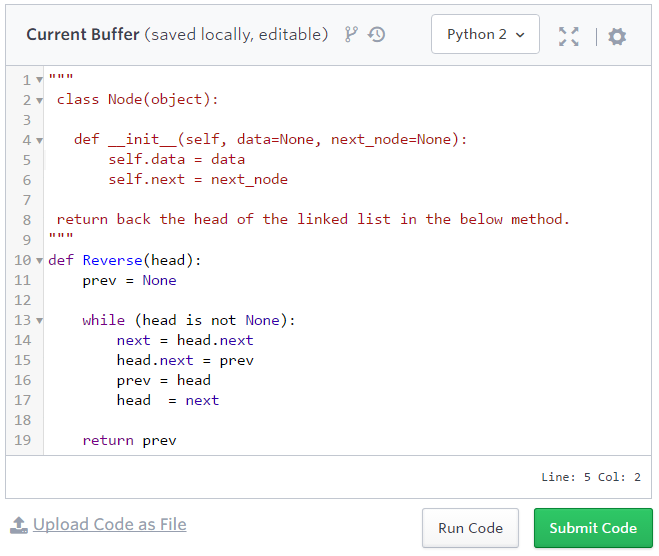
\includegraphics[width=\textwidth, trim=20 20 0 30]{img/hackerrank.png}
        \captionsetup{width=\textwidth, justification=centering}
        \captionof{figure}{Code editor from HackerRank\cite{hrlinkedlist}}\label{fig:hrlinkedlist}
      \end{minipage}%
      \quad
      \begin{minipage}{.48\textwidth}
        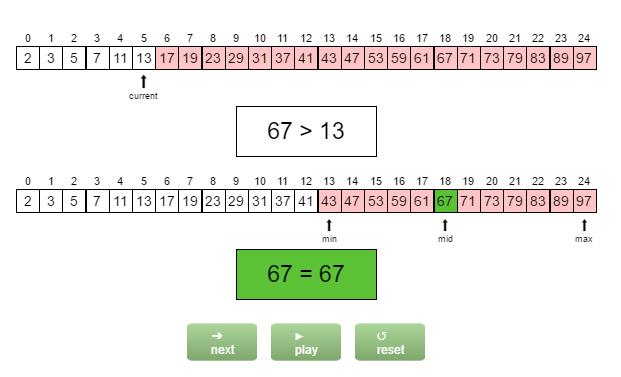
\includegraphics[width=\textwidth, trim=0 -37 0 -37]{img/khansearch.png}
        \captionsetup{width=\textwidth, justification=centering}
        \captionof{figure}{Binary search visualisation from Khan Academy\cite{khanbinsearch}}\label{fig:khanbinsearch}
      \end{minipage}
    \end{figure}

    \section{Simulators as a Teaching Aid}\label{sec:mustafa-simulator}

    In his article {\em Evaluating A System Simulator For Computer
      Architecture Teaching And Learning Support}\cite{mustafa2010},
    Mustafa discusses the design \& implementation of a system
    which integrates the simulation of a compiler, CPU and operating
    system to aid in the teaching of undergraduate computer
    architecture and operating systems modules.

    Although brief, the article provides valuable insight into the
    design and evaluation of such teaching software. The primary
    source of feedback came from an opinion survey using a 5-point
    \gls{likertscale} for quantitative analysis and open-ended questions
    for qualitative feedback. In addition, students were administered
    a test to assess their knowledge pre- and post- use of the system.

    The evaluation results highlight an important point to consider
    when designing teaching software; over 20\% of respondents
    indicated that they spent more time learning how to use the
    software than they did completing the given exercises. An equal
    number of students reported that the simulator left them more
    confused than before. In addition, 7.1\% of respondents said that
    the simulator was too complicated to use effectively in their
    tutorials.

    However, the converse of these results gives a positive outlook
    for this project: 72.4\% of respondents disagreed with the above
    statements and 79.3\% believed that the system improved their
    understanding of the topics covered in lectures. Over 95\% of
    responents agreed that the simulator was more useful than reading
    textbooks or searching the internet in helping them understand the
    material.

    \section{Learning and Teaching Styles}

    A 1988 report by Richard M. Felder and Linda K. Silverman,
    entitled {\em Learning and Teaching Styles in Engineering
      Education}\cite{felder1988}, categorizes students' learning
    methods and describes ways in which professors may target specific
    categories in their teaching strategy.

    Felder refers to the learning modalities (or VAK) model proposed
    by Walter Burke Barbe, which defines three modalities:

    \begin{itemize}
    \item {\bf visual} -- those who learn best by viewing images and
      diagrams;
    \item {\bf auditory} -- those who learn best by listening or
      speaking aloud; and
    \item {\bf kinaesthetic} -- those who learn best by actively
      experiencing things, learning by doing.
    \end{itemize}

    The report claims that most people of college age and above, the
    intended audience of this project, identify as {\em visual}
    learners -- those who benefit from charts, diagrams and such. In
    contrast, the presentation of content in university courses is
    primarily {\em auditory} (via lectures) or a visual representation
    of auditory information (i.e. words or mathematical formulae).

    The survey results from Mustafa\cite[p. 103]{mustafa2010} support this
    observation: although only a small sample (N=54) responded, 31\%
    of respondents identified as visual learners, while a mere 6\%
    identified as auditory learners. The majority of students (52\%)
    identified as kinaesthetic learners, indicating that taking a
    hands-on approach is a valuable tool for learning.

    It should be noted that Felder discounts kinaesthetic learning
    from his report as he considers the {\em learning by doing} to be
    a separate category, perceiving the remaining attributes of
    kinaesthetic learning to have little value in engineering. A later
    observation by Felder agrees with Mustafa, stating that engineers
    are ``more likely to be active than reflective learners''
    \cite[p. 678]{felder1988}.

        \subsection{Ability to Identify Own Learning Style}

        In her PhD dissertation {\em ``Individual Differences in
          Learning: Predicting One's More Effective Learning
          Modality''} \cite{farr1970}, Beatrice J. Farr claims that
        students are able to accurately predict the learning style in
        which they perform best:

        \begin{quote}
          ``An experiment with 72 college students confirmed that
          individuals could accurately predict the modality in which
          they could demonstrate superior learning performance. The
          data also revealed that it is advantageous to learn and be
          tested in the same modality and that such an advantage is
          reduced when learning and testing are both conducted in an
          individual's preferred modality.''\cite[p. 242]{dunn1979}
        \end{quote}

        Coffield\cite[p. 120]{coffield2004} disagrees with this, based
        on an observation by Merrill\cite{merrill2000} that ``most
        students are unaware of their learning styles and so, if they
        are left to their own devices, they are most unlikely to start
        learning in new ways''. This would indicate that basing
        teaching methods on a student's preferences is damaging to
        their education. This is, however, a misinterpretation; the
        actual text of Merrill reads:

        \begin{quote}
          ``... a student must engage in those activities ... that are
          required for them to acquire a particular kind of knowledge
          or skill ... Most students are unaware of these fundamental
          instructional (learning) strategies and hence left to their
          own are unlikely to engage in learning activities most
          appropriate for acquiring a particular kind of knowledge or
          skill.''\cite[p. 4]{merrill2000}
        \end{quote}

        Merrill later argues that the optimal strategy for teaching is
        decided first and foremost by the content being taught, then
        fine-tuned to the learner's preferred style
        \cite[p. 4]{merrill2000}. By not knowing the most effective
        strategy for learning the content they are studying, a student
        limits his or her potential. However, the appropriate strategy
        {\em should} in fact be tailored to the student's preferred
        learning style to obtain the best results.

        \subsection{Criticism of Learning Modalities}\label{sec:matching}

        Some of the criticism levied at the concept of learning styles
        is that the idea of {\em matching} -- exclusively teaching a
        student based on his or her preferred learning style -- is
        harmful to a student's education. Although Coffield's
        \cite[p. 120]{coffield2004} reasoning is flawed, the
        conclusion drawn by him and Merrill \cite[p. 4]{merrill2000}
        is sound: by allowing students to exclusively use their
        preferred way of learning, students are at risk of missing out
        on more effective methods of study.

        Felder's report mentions a study carried out by the
        Socony-Vacuum Oil Company, which concludes that:

        \begin{quote}
          ``...students retain 10 percent of what they read, 26
          percent of what they hear, 30 percent of what they see, 50
          percent of what they see and hear, 70 percent of what they
          say, and 90 percent of what they say as they do
          something.''\cite[p. 677]{felder1988}
        \end{quote}

        This indicates that by relying solely upon auditory methods,
        professors can only hope to convey as little as 26\% of the
        desired material to their students. Felder advocates using a
        mixture of teaching methods in order to appeal to all
        students' preferred learning styles.

    \section{Summary}

    While there may be some disagreement over the validity of learning
    styles or modalities, even its critics seem to agree that there is
    value in varying the methods of teaching in use. At present, the
    only available resources for learning \gls{dataflowanalysis} are
    lecture slides, videos and textbooks. These are mostly auditory
    and sometimes visual methods of teaching, with little kinaesthetic
    learning involved. There is a clear need for more active study;
    although 52\% of students identified as learning best through
    kinaesthetic learning\cite[p. 103]{mustafa2010}, there is almost
    no support for this method of study.

    Given the relative success of the examples discussed in this
    chapter and the apparent lack of any such resources for
    \gls{dataflowanalysis}, there is a strong precedent for this
    project and as such a system will be developed to fulfil this
    role.

    However, it is important to note the mistakes made by the examples
    discussed here. The simulator designed by Mustafa was deemed too
    complex\cite[p. 103]{mustafa2010} and a detriment to their
    learning by over 20\% of respondents. This project will seek to
    ensure that that content is clear and concise on order to produce
    an effective learning resource.

    To evaluate the success of the system this project will build upon
    the methods presented by Mustafa, aggregating opinion using a
    \gls{likertscale} and examining this data to judge overall
    satisfaction with the software and identify specific areas for
    improvement.


\chapter{Design}
This chapter discusses the high-level design and architecture of the
system, including motivations for design choices and solutions to
conceptual problems.

    \section{Introduction}
    The original goal of this project was to produce an online
    simulation of \gls{dataflowanalysis} to show students how
    data-flow works. As discovered in the related reading, however, a
    large portion of users of a similar system found it to be too
    complex and claimed to have spent more time studying the software
    itself than the topic at hand. The literature also raised another
    key point; a wide variety of learning techniques are necessary to
    gain a true understanding of a topic.

    For these reasons the proposal has been extended to create a
    comprehensive learning platform. In addition to the simulator the
    software will provide supporting lectures to explain the basic
    concepts and gradually introduce each element of the
    simulation. These lectures will include visual and interactive
    elements to engage the user through a range of learning styles. It
    is hoped that the system will prove a valuable tool for learning
    alongside existing resources such as textbooks and lectures.

    \section{Design Constraints}
    In this section, design constraints are identified and potential
    solutions are suggested.

        \subsection{Technical Constraints}
        As the intention isto make such a system available to
        \gls{copt} students via the University, the following
        technical considerations must be made:

        \begin{itemize}
        \item The system must be distributed to all students in some format;
        \item This format must be functional on and compatible with a
          wide range of devices owned by said students;
        \item The system must be secure and require little
          maintenance; and
        \item The system must be hosted on some platform available to
          the University.
        \end{itemize}

        In order to meet these criteria the system must rely on as
        little technology as possible. The easier the platform is to
        host and distribute, the more likely it is to be made
        available to students -- a system which uses new technology
        and requires its own dedicated hosting would be more difficult
        to set up and maintain than one which can be deployed to
        existing hardware. It is necessary to ensure that the system
        is secure to avoid damaging University or student property.

        The application could be developed using purely client-side
        technologies such as JavaScript, HTML and CSS. These static
        files may be distributed over HTTP using any standard web
        server such as the one already used to host the course
        webpage. Efforts must be made to keep the performance of the
        system consistent across a range of web browsers and devices;
        although all modern web browsers are capable of interpreting
        these types of content there are subtle differences which may
        break functionality on one platform but not others.

        Use of popular libraries and frameworks such as jQuery and
        Bootstrap will be encouraged as this provides a number of
        benefits. The user will experience reduced load times since
        they have likely already downloaded the required files, and
        such libraries will provide security and robustness due to
        their wide use and active development. Likewise, the more
        popular a library is the more documentation and resources will
        be available to aid in developing the best possible system.
        
        The specific technologies used in each are detailed in the
        implementation (chapters \ref{chap:impl-backend} \&
        \ref{chap:impl-frontend}).

          
        \subsection{Content Constraints}
        To be viable as a learning platform, the system must:
        
        \begin{itemize}
        \item Appeal to a range of learning styles;
        \item Provide comprehensive coverage of the topic at hand;
        \item Ensure the content included is correct, clear and
          concise; and
        \item Maintain a shallow learning curve, gradually introducing
          students to each topic or element of the simulation.
        \end{itemize}

        Extending the proposed system into a comprehensive learning
        platform will provide a range of ways in which to study
        \gls{dataflowanalysis}. Students will have the choice to use
        the areas of the software which most appeal to them and
        content will be presented using a mixture of interactive,
        visual and textual formats.

        As the aim is to assist students of the \gls{copt} course,
        coverage of topics will be prioritised based on their
        inclusion in the course syllabus and whether they are required
        to understand the simulation:

        \begin{itemize}
        \item Basic principles of data-flow analysis;
        \item A few simple data-flows, including:
          \begin{itemize}
          \item Reaching Definitions
          \item Liveness Analysis
          \item Available Expressions
          \end{itemize}
        \item Round-robin fixed-point algorithm;
        \item Effect of orderings on analysis efficiency;
        \item Generic frameworks for data-flow analysis;
        \item Hasse diagrams and lattice representation of values; and
        \item Conditions for analysis termination.
        \end{itemize}        

        If the content delivered by the platform is incomplete,
        incorrect or too difficult to understand, the system will not
        present a viable alternative method of study. When evaluating
        the system it will be important to assess the clarity and
        presentation of the material, and the ease of use of the
        platform as a whole.


    \section{System Architecture}
    This system is divided into two main areas of development.  The
    back-end of the system controls the logic and state of a data-flow
    analysis simulation. The front-end components will hook into and
    expose elements of the back-end, visualising the state of the
    simulation and allowing the user to interact with it. See
    fig. \ref{fig:sysarch} for a visual representation.
    
    Object-oriented design will be paramount, allowing functionality
    to be extended and shared between similar elements. In addition to
    speeding up development of the system by reducing the need to
    duplicate code, this is generally good design practice. Components
    will be written as re-usable modules which can be combined in
    different ways, for example to present the user with a series of
    lectures or an interactive simulation. See
    \S\ref{sec:design-interface} for more details on the user
    interface.

    Each component needs to be be self contained; it should be
    possible to instantiate more than one of each type of component at
    once, including the simulator itself. This would allow, say,
    displaying the annotated control-flow graphs of two simulations
    side-by-side. The simulation will also be independent of the user
    interface so that it may be adapted for re-use in other projects.
   
    \begin{figure}[!ht]
      \centering
      \scalebox{0.8}{
        \begin{tikzpicture}[x=1mm, y=-1mm,
          person/.pic={%
            \node (-head) [circle, minimum size=4*\pgfkeysvalueof{/cfr/soul base dimension}] {};
            \node (-torso) [below=0pt of -head, rectangle, rounded corners=.4*\pgfkeysvalueof{/cfr/soul base dimension}, minimum width=3.5*\pgfkeysvalueof{/cfr/soul base dimension}, minimum height=6*\pgfkeysvalueof{/cfr/soul base dimension}] {};
            \node (-right arm) [right=0pt of -torso.north east, yshift=-3.1*\pgfkeysvalueof{/cfr/soul base dimension}, rectangle, minimum width=\pgfkeysvalueof{/cfr/soul base dimension}, minimum height=6*\pgfkeysvalueof{/cfr/soul base dimension}, rounded corners=.4*\pgfkeysvalueof{/cfr/soul base dimension}] {};
            \node (-left arm) [left=0pt of -torso.north west, yshift=-3.1*\pgfkeysvalueof{/cfr/soul base dimension}, rectangle, minimum width=\pgfkeysvalueof{/cfr/soul base dimension}, minimum height=6*\pgfkeysvalueof{/cfr/soul base dimension}, rounded corners=.4*\pgfkeysvalueof{/cfr/soul base dimension}] {};
            \node (-left leg) [below=0pt of -torso.south, rectangle, minimum width=1.5*\pgfkeysvalueof{/cfr/soul base dimension}, minimum height=6*\pgfkeysvalueof{/cfr/soul base dimension}, rounded corners=.2*\pgfkeysvalueof{/cfr/soul base dimension}, anchor=north east] {};
            \node (-right leg) [below=0pt of -torso.south, rectangle, minimum width=1.5*\pgfkeysvalueof{/cfr/soul base dimension}, minimum height=6*\pgfkeysvalueof{/cfr/soul base dimension}, rounded corners=.2*\pgfkeysvalueof{/cfr/soul base dimension}, anchor=north west] {};
            \draw [rounded corners=.2*\pgfkeysvalueof{/cfr/soul base dimension}] (-right leg.south) -- (-right leg.south west) -- (-left leg.south east) -- (-left leg.south west)  -- (-torso.south west) [rounded corners=.4*\pgfkeysvalueof{/cfr/soul base dimension}] -- (-left arm.south east) -- (-left arm.south west) -- (-left arm.north west) -- (-torso.north west) -- ($(-head.south) - (.5*\pgfkeysvalueof{/cfr/soul base dimension},0)$) arc [start angle=255.5, end angle=-74.5, radius=2*\pgfkeysvalueof{/cfr/soul base dimension}] -- (-torso.north east) -- (-right arm.north east) -- (-right arm.south east)  -- (-right arm.south west) [rounded corners=.2*\pgfkeysvalueof{/cfr/soul base dimension}] -- (-torso.south east)  -- (-right leg.south east) -- (-right leg.south west);
          }
          ]
          % vertices
          \tikzstyle{group} = [rectangle, draw, text centered, rounded corners, dash pattern=on 2pt off 3pt, below right]
          \tikzstyle{cluster} = [rectangle, draw, text width=60mm, text centered, rounded corners, densely dotted, below right]
          \tikzstyle{clusterlabel} = [text width=60mm, minimum height=10mm, text centered, below]
          \tikzstyle{component} = [rectangle, draw, text width=50mm, text centered, rounded corners, minimum height=7mm, below right]

          \node[group, text width=135mm, minimum height=56mm] (backend) at (0,0) {};
          \node[clusterlabel, text width=100mm] at (backend.north) {Back-end Components};

          \node[cluster, minimum height=42mm, below = 10mm of backend.north] (simulator) {};
          \node[clusterlabel] at (simulator.north) {Simulator};
          \node[component, below=10mm of simulator.north] (sfwk)  {Data-Flow Framework};
          \node[component, below=20mm of simulator.north] (scfg)  {Program CFG};
          \node[component, below=30mm of simulator.north] (salgo) {Analysis Algorithm};

          \node[group, text width=135mm, minimum height=76mm, below=5mm of backend.south] (frontend) {};
          \node[clusterlabel, text width=100mm] at (frontend.north) {Front-end Components};

          \node[cluster, minimum height=62mm, below left=10mm and 2mm of frontend.north] (visual) {};
          \node[clusterlabel] at (visual.north) {Visual Components};
          \node[component, below=10mm of visual.north] (vcfg)   {Visual CFG};
          \node[component, below=20mm of visual.north] (vhasse) {Hasse Diagram};
          \node[component, below=30mm of visual.north] (vres)   {Table of Results};
          \node[component, below=40mm of visual.north] (vlst)   {Code Listing};
          \node[component, below=50mm of visual.north] (vfwk)   {Framework Properties};

          \node[cluster, minimum height=52mm, below right=10mm and 2mm of frontend.north] (interface) {};
          \node[clusterlabel] at (interface.north) {Interactive Components};
          \node[component, below=10mm of interface.north] (imenu) {Navigation};
          \node[component, below=20mm of interface.north] (itext) {Text Pages};
          \node[component, below=30mm of interface.north] (iques) {Questions};
          \node[component, below=40mm of interface.north] (icont) {Simulation Controls};
          
          \pgfkeyssetvalue{/cfr/soul base dimension}{5pt}
          \pic (user) [below=5mm of frontend.south] {person};

          % \draw[edge] (simulator) .. controls ([xshift=-4cm] simulator) and ([xshift=4cm] visual) .. (visual);

          \draw[-{>[scale=2.5]}] ($ (interface.north) + (8, 0) $) |- (simulator.east) node [near start, right, text width=30mm, text centered] {\footnotesize User actions update simulation};
          \draw[-{>[scale=2.5]}] (simulator.west) -| ($ (visual.north) +  (-8, 0) $) node [near end, left, text width=25mm, text centered] {\footnotesize Updates propagated to visual components};
          \draw[-{>[scale=2.5]}] ($ (user-right arm.east) + (2, 0)$) -| ($ (interface.south) + (8,0) $) node [midway, above right, text width=28mm, text centered] {\footnotesize User interacts with front-end};
          \draw[-{>[scale=2.5]}] ($ (visual.south) + (-8, 0) $) |- ($ (user-left arm.west) + (-2, 0)$) node [midway, above left, text width=28mm, text centered] {\footnotesize User receives visual feedback};
        \end{tikzpicture}
      }
      \captionsetup{justification=centering}
      \caption{An overview of the planned system architecture.}\label{fig:sysarch}
    \end{figure}


    \section{User Interface Design}\label{sec:design-interface}

    

%%%%%%%%%%%%%%%%%%%%%%%%%%%%%%%%%%%%%%%
\chapter{Back-End Implementation}\label{chap:impl-backend}
This chapter discusses the implementation of the
\gls{dataflowanalysis} simulation -- the back-end elements which
control the logic and state of the analysis, which is then presented
by the user interface components described in chapter
\ref{chap:impl-frontend}.

    \section{Overview}
    The implementation of the simulator is based upon the concept of a
    general framework as described in
    \S\ref{sec:background-frameworks} of this report and \S10.11 of
    the {\em Dragon Book}\cite{dragonbook}. The simulator takes as
    input a program written in the \gls{iloc} language, a
    \gls{dataflow} framework and an order in which to evaluate
    nodes. It parses the program into an \gls{ast} and uses this to
    build a \gls{cfg}, then performs an analysis on said graph using
    the round-robin \gls{fixedpoint} algorithm for general frameworks
    (algorithm \ref{algo:general}).

    Playback of the simulation can be controlled through the
    simulator's \gls{api}. Function calls which update the state of
    the simulation trigger an event handling system to update the
    visual components. However, the simulation is entirely independent
    of the rest of the system; re-using it in another project is as
    simple as copying the directory containing the simulator code and
    including the required libraries.

    The simulator is implemented entirely in JavaScript. Snippets of
    code taken from external sources are explicitly commented as such
    in the source code and will be mentioned here.

    \section{Value Sets}

    JavaScript includes a native {\tt Set} data structure for
    representing collections of unique objects. Unfortunately, two
    objects are only seen as equal if they refer to the exact same
    instance. For the purposes of this simulation it would be useful
    to compare objects which share some attributes but refer to
    different instances; for example, when operating on sets of
    operands it would be useful to consider two operands of different
    instructions as the same if they refer to the same variable.

    For this reason the simulator uses a new {\tt ValueSet} data
    structure, backed by a native JavaScript {\tt array}. The {\tt
      ValueSet} stores objects which inherit from a {\tt
      ValueMixin}\footnote{A mixin class contains methods which may be
      inherited by another class, but is not necessarily the parent of
      that class.} and must define a {\tt compare} function. Objects
    are checked for equality using this function so that two objects
    may be considered equal based on selected attributes.

    {\tt ValueSet}s support the following operations, listed here
    along with their estimated worst-case time complexities:

    \begin{table}[!ht]
      \centering
      \def\arraystretch{1.2}
      \scalebox{0.9}{
      \begin{tabularx}{0.8\textwidth}{|C|C|C|C|}
        \hline
            {\tt s.size()} & {\tt s.add(v)} & {\tt s.delete(v)} & {\tt s.has(v)} \\ \hline
            $O(1)$         & $O(|s|)$       & $O(|s|)$          & $O(|s|)$       \\ \hline
      \end{tabularx}
    }
      \\[2mm]
      \scalebox{0.9}{
      \begin{tabularx}{0.8\textwidth}{|C|C|C|}
        \hline
            {\tt s.union(t)}   & {\tt s.intersect(t)} & {\tt s.difference(t)} \\ \hline
            $O(|s| \cdot |t|)$ & $O(|s| \cdot |t|)$   & $O(|s| \cdot |t|)$    \\ \hline
      \end{tabularx}
    }
    \end{table}

    Using an alternate backing structure such as a hash table would
    provide constant-time implementations of {\tt has}, {\tt add} and
    {\tt delete}, and thus also improve the run-time of operations
    which make use of these functions ({\tt union}, {\tt intersect}
    and {\tt difference}). Given that the expected user input will
    only operate on small {\tt ValueSet}s this is not a major concern,
    but a potential improvement that should be noted for future
    development.
    
    \section{Data-Flow Frameworks}
    
    Each data-flow framework defines the elements outlined in
    \S\ref{sec:background-frameworks}, namely:

    \begin{itemize}
    \item The {\em \gls{domain}} of values on which to operate;
    \item The {\em \gls{direction}} in which data flows;
    \item A set of {\em \gls{dataflowequations}} including the {\em
        \gls{meetoperator}} $\land$ and the set of {\em
        \gls{transfer} functions} $F$.
    \item The {\em \gls{boundary}} value specifying the initial value
      at the entry or exit to the \gls{cfg}; and
    \item The {\em initial value}, $\top$, at each point in the graph.
    \end{itemize}

    The meet and transfer functions operate on {\tt
      ValueSets}. Frameworks must also specify the following additional
    information:

    \begin{itemize}
    \item A name and identifier;
    \item \LaTeX\ representations of the \gls{meet} and \gls{transfer} functions; and
    \item JavaScript functions to compute local information
      independent from the \gls{transfer} function.
    \end{itemize}

    This allows properties of the framework to be displayed by the
    visual components in addition to the values calculated at each
    point.
    
    \section{Simulation Algorithm}
    Algorithm \ref{algo:general_impl} shows a disassembled version of
    algorithm \ref{algo:general}. The functions can be combined to
    enable a step-by-step evaluation or automatic playback.

    \begin{algorithm}[caption={Implementation of General Framework Algorithm}, label={algo:general_impl},escapeinside={||},mathescape=true]
function reset()
    B = entry node of CFG
    B.meet = framework.boundary
    for each (node in the cfg)
        node.meet = framework.top
    step    = |{\tt MEET}|
    changed = false

function iterate()
    if (step is |{\tt MEET}|)
        B.meet, changed = framework.meet(b, this.cfg)
        step = |{\tt TRANSFER}|
    else
        B.transfer, changed = framework.transfer(b)
        step = |{\tt MEET}|
        B    = next node
    \end{algorithm}

    To demonstrate, listings and \ref{lst:fast_forward} and
    \ref{lst:autoplay} show the implementation of some of the playback
    functions. In the fast forward function, the simulation is
    advanced until it is complete before triggering an update event
    which is propagated to other components of the system. In the
    automatic playback function, a function is called at set time
    intervals which advances the simulation by one iteration, then
    triggers the update. Controlling when update events are triggered
    events helps prevent slowdown from unnecessary re-rendering of
    components.

    \begin{figure}[!ht]
      \begin{lstlisting}[language=JavaScript, caption={JavaScript Implementation of Fast Forward}, label={lst:fast_forward}]
this.fast_forward = function() {
  while(!this.state.finished) {
    this.iterate();
  }
  this.events.trigger('update');
}
      \end{lstlisting}
    \end{figure}

    \begin{figure}
      \begin{lstlisting}[language=JavaScript, caption={JavaScript Implementation of Automatic Playback}, label={lst:autoplay}]
this.play = function() {
  this.state.paused = false;
  var _this = this;
  (function foo() {
    if (!_this.state.paused && !_this.state.finished) {
      // If the user hasn't pressed pause and we're not finished
      _this.iterate();                   // Step forward
      _this.events.trigger('update');    // Update components
      setTimeout(foo, _this.play_speed); // Repeat at interval
    }
  })();
}
      \end{lstlisting}
    \end{figure}
    
    \section{Understanding Programs}
    The simulation operates on programs written in \gls{iloc}, as
    described in {\em Engineering a Compiler}
    \cite[appx.~A]{eac}. \gls{iloc} is an assembly-like language
    designed for toy compilers as it is both simple to parse and
    human-readable. This makes it the perfect input language for the
    learning platform, with the added benefit that students will be
    able to step through examples from the textbook using the
    simulator.

    The simulator supports the following ILOC features:

    \begin{itemize}
    \item The entire set of opcodes listed in {\em Engineering a
        Compiler};
    \item Three types of literal: registers, labels, and integers;
    \item Simple programs with a single operation per instruction; and
    \item Distinction between three types of memory: registers, main
      memory, and the comparison register.
    \end{itemize}

    There is also limited support for multi-operation instructions,
    which may be used to emulate \gls{dataflowanalysis} on basic
    blocks. This functionality remains untested as priority was
    assigned to simulation on nodes as single instructions.

    \glsreset{ast}

    In order to understand ILOC programs, they must be to converted
    from text into a \gls{cfg}. To do this the simulator uses the
    PEG.js\cite{pegjs} library which, given an input grammar,
    generates a parser written in JavaScript. This parser produces an
    \gls{ast}, which is then transformed into a \gls{cfg} representing
    the program. The following sections describe this process in more
    detail.

        \subsubsection{Parsing Expression Grammar}\label{sec:peg}

        A \gls{peg} is very similar to a \gls{contextfreegrammar} in
        that it describes a formal language using a set of rules for
        recognising strings in that language. The description of
        \gls{iloc} in {\em Engineering a Compiler} describes a simple
        \gls{peg} for the language, which has been adapted for use in
        this system.
        
        The rules of the grammar have been extended as shown in
        fig. \ref{fig:grammar_extensions}. The reason for these
        changes is that \gls{iloc} allows the user to write to three
        types of storage: registers, main memory and comparison
        flags. Changing the grammar allows disambiguation in the
        abstract syntax tree between operations which write to or read
        from different types of storage. This is an important
        distinction to make because the built-in data-flows only
        consider register accesses when calculating value sets at each
        point (see \S\ref{sec:builtin_dataflows} for an explanation).

        The full extended \gls{iloc} grammar is listed in appendix
        \ref{appx:iloc_grammar}.

        \begin{figure}[!ht]
          \centering
          \scalebox{0.9}{
          \begin{tabular}{M{r} M{c} M{l} M{l} M{l} M{l}}
            Operation         & \rightarrow & NormalOp          &             &             &             \\
                              & |           & ControlFlowOp     &             &             &             \\
                              & |           & MemoryLoadOp      &             &             &             \\
                              & |           & MemoryStoreOp     &             &             &             \\
                              &             &                   &             &             &             \\
            MemoryLoadOp      & \rightarrow & LoadOpcode        & OperandList & \Rightarrow & OperandList \\
            MemoryStoreOp     & \rightarrow & StoreOpcode       & OperandList & \Rightarrow & OperandList \\
            NormalOp          & \rightarrow & NormalOpcode      & OperandList & \Rightarrow & OperandList \\
            ControlFlowOp     & \rightarrow & ControlFlowOpcode & OperandList & \Rightarrow & OperandList \\
                              &             &                   &             &             &             \\
            LoadOpcode        & \rightarrow & \texttt{loadI}    &             &             &             \\
                              & |           & \texttt{loadAO}   &             &             &             \\
                              & |           & ...               &             &             &             \\
                              &             &                   &             &             &             \\
            StoreOpcode       & \rightarrow & \texttt{storeI}   &             &             &             \\
                              & |           & \texttt{storeAO}  &             &             &             \\
                              & |           & ...               &             &             &             \\
                              &             &                   &             &             &             \\
            NormalOpcode      & \rightarrow & \texttt{addI}     &             &             &             \\
                              & |           & \texttt{rshift}   &             &             &             \\
                              & |           & ...               &             &             &             \\
                              &             &                   &             &             &             \\
            ControlFlowOpcode & \rightarrow & \texttt{jumpI}    &             &             &             \\
                              & |           & \texttt{cbr\_GE}  &             &             &             \\
                              & |           & ...               &             &             &             \\
                              &             &                   &             &             &             \\
            Operand           & \rightarrow & register          &             &             &             \\
                              & |           & num               &             &             &             \\
                              & |           & label             &             &             &             \\
                              & |           & cc                &             &             &             \\
                              &             &                   &             &             &             \\
            cc                & \rightarrow & \texttt{cc}       &             &             &             \\
          \end{tabular}
        }
          \caption{Extensions to \gls{iloc} Parsing Expression Grammar}\label{fig:grammar_extensions}
        \end{figure}

        \subsection{Abstract Syntax Tree}

        A parse tree represents the exact structure of parsed data. In
        contrast, an \gls{ast} represents the structure of data
        independent of its original representation; this may involve
        adding or removing nodes or re-structuring the tree entirely.

        To construct an \gls{ast} one would usually obtain a parse
        tree and then transform it into the desired structure. Parsers
        generated by the PEG.js library are capable of constructing
        the \gls{ast} as they parse the input program. The developer
        may supply JavaScript code to be executed when a rule matches
        and this code is used to create an abstract representation of
        the data matched by that rule. This feature can also be used
        to annotate the tree as it is built.

        \begin{figure}[!ht]
          \begin{lstlisting}[language=JavaScript, caption=Example of PEG.js Grammar Rules, escapeinside={||}, label=lst:peg_grammar]
Operand
    = _ r:register _ { return r; }|\label{ln:returnval}|
    / _ n:num _ { return n; }      
    / _ c:cc _ { return c; }       
    / _ l:label _ { return l; }    
                                   

register
    = _ "r" n:([0-9a-z_]i)+ _ {|\label{ln:identifier}|
        return new ILOC.Operand({
            type: ILOC.OPERAND_TYPES.register,
            name: n.join("")|\label{ln:nameassignment}|
        });
    }
          \end{lstlisting}
        \end{figure}

        Listing \ref{lst:peg_grammar} shows a snippet of the PEG.js
        grammar for \gls{iloc}. Groups of symbols may be assigned an
        identifier and referred to in the JavaScript code; on line
        \ref{ln:identifier} the identifier {\tt n} is given to the
        register name so it can be set as the name of the returned
        {\tt Operand}. The return value of the JavaScript code is
        passed to the above context; the identifier {\tt r} on line
        \ref{ln:returnval} refers to the {\tt Operand} returned by the
        {\tt register} rule. More complex code may collect information
        and use it to annotate the AST; for example, the grammar used
        in this project annotates assignments to a given register with
        a unique identifier for use in \gls{dataflow}s such as
        \gls{reachingdefinition}s.

        Fig. \ref{fig:iloc_ast} shows an example \gls{ast} for the
        simple \gls{iloc} program in listing \ref{lst:iloc_ast_code}.

        \begin{figure}[!ht]
        \begin{lstlisting}[language=ILOC, caption=Simple \gls{iloc} Program, label=lst:iloc_ast_code]
Start: addI    ra, 1  => rb
       comp    ra, rb => cc
       cbr_LE  cc     -> Start, Store
Store: storeAO ra     => rx, 32
        \end{lstlisting}
        \end{figure}

        \begin{figure}[p]
          \centering
          \begin{tikzpicture}[x=1mm, y=-1mm]
            
            \node[tree] (ilocprogram) at (0,0) {IlocProgram};


              \node[tree, below right=4mm and 20mm of ilocprogram.south west] (i1) {Instruction};

                \node[atom, right=16mm of i1.east] (i1label) {Start};

                \node[tree, below right=6mm and 20mm of i1.south west] (i1op1) {NormalOperation};

                  \node[atom, right=16mm of i1op1.east] (i1op1oc) {addI};

                  \node[tree, below right=12mm and 0mm of i1op1.south west] (i1op1s1) {Operand};
                    \node[atom, below left=8mm and -4mm of i1op1s1.south] (i1op1s1type) {register};
                    \node[atom, below right=8mm and 8mm of i1op1s1.south] (i1op1s1name) {a};

                  \node[tree, right=12mm of i1op1s1] (i1op1s2) {Operand};
                    \node[atom, below left=8mm and 1mm of i1op1s2.south] (i1op1s2type) {num};
                    \node[atom, below right=8mm and 3mm of i1op1s2.south] (i1op1s2name) {1};

                  \node[tree, right=17mm of i1op1s2] (i1op1t1) {Operand};
                    \node[atom, below left=8mm and 2mm of i1op1t1.south] (i1op1t1type)  {register};
                    \node[atom, below right=8mm and 2mm of i1op1t1.south] (i1op1t1name)  {a};
                    \node[atom, below right=8mm and 12mm of i1op1t1.south] (i1op1t1index) {1};


              \node[tree, below right=62mm and 20mm of ilocprogram.south west] (i2) {Instruction};

                \node[tree, below right=6mm and 20mm of i2.south west] (i2op1) {NormalOperation};

                  \node[atom, right=16mm of i2op1.east] (i2op1oc) {comp};

                  \node[tree, below right=12mm and 0mm of i2op1.south west] (i2op1s1) {Operand};
                    \node[atom, below left=8mm and -4mm of i2op1s1.south] (i2op1s1type) {register};
                    \node[atom, below right=8mm and 8mm of i2op1s1.south] (i2op1s1name) {a};

                  \node[tree, right=17mm of i2op1s1] (i2op1s2) {Operand};
                    \node[atom, below left=8mm and 1mm of i2op1s2.south] (i2op1s2type) {num};
                    \node[atom, below right=8mm and 3mm of i2op1s2.south] (i2op1s2name) {b};

                  \node[tree, right=12mm of i2op1s2] (i2op1t1) {Operand};
                    \node[atom, below= 8mm of i2op1t1.south] (i2op1t1type)  {cc};

                \node[tree, below right=52mm and 20mm of i2.south west] (i2op2) {ControlFlowOperation};

                  \node[atom, right=16mm of i2op2.east] (i2op2oc) {cbr\textunderscore{}LE};

                  \node[tree, below right=12mm and 0mm of i2op2.south west] (i2op2s1) {Operand};
                    \node[atom, below=8mm of i2op2s1.south] (i2op2s1type) {cc};

                  \node[tree, right=12mm of i2op2s1] (i2op2t1) {Operand};
                    \node[atom, below left=8mm and 2mm of i2op2t1.south] (i2op2t1type) {label};
                    \node[atom, below right=8mm and 2mm of i2op2t1.south] (i2op2t1name) {Start};

                  \node[tree, right=17mm of i2op2t1] (i2op2t2) {Operand};
                    \node[atom, below left=8mm and 2mm of i2op2t2.south] (i2op2t2type) {label};
                    \node[atom, below right=8mm and 2mm of i2op2t2.south] (i2op2t2name) {Store};


              \node[tree, below right=166mm and 20mm of ilocprogram.south west] (i3) {Instruction};

                \node[atom, right=16mm of i3.east] (i3label) {Store};

                \node[tree, below right=8mm and 20mm of i3.south west] (i3op1) {MemoryStoreOperation};

                  \node[atom, right=16mm of i3op1.east] (i3op1oc) {storeAO};

                  \node[tree, below right=12mm and 0mm of i3op1.south west] (i3op1s1) {Operand};
                    \node[atom, below left=8mm and -4mm of i3op1s1.south] (i3op1s1type) {register};
                    \node[atom, below right=8mm and 8mm of i3op1s1.south] (i3op1s1name) {a};

                  \node[tree, right=17mm of i3op1s1] (i3op1t1) {Operand};
                    \node[atom, below left=8mm and -4mm of i3op1t1.south] (i3op1t1type) {register};
                    \node[atom, below right=8mm and 8mm of i3op1t1.south] (i3op1t1name) {x};

                  \node[tree, right=12mm of i3op1t1] (i3op1t2) {Operand};
                    \node[atom, below left=8mm and 1mm of i3op1t2.south] (i3op1t2type) {num};
                    \node[atom, below right=8mm and 3mm of i3op1t2.south] (i3op1t2name) {32};

          %% Edges
          \draw[-{>[scale=1.5]}] ($(ilocprogram.south) + (-8, 0)$) |- (i1.west);

            \draw[-{>[scale=1.5]}] (i1.east) -- (i1label.west) node [midway, above, text centered] {\footnotesize\it label};

            \draw[-{>[scale=1.5]}] ($(i1.south) + (-4, 0)$) |- (i1op1.west) node [near start, left, text centered] {\footnotesize\it operations};
              \draw[-{>[scale=1.5]}] (i1op1.east) -- (i1op1oc.west) node [midway, above, text centered] {\footnotesize\it opcode};

              \draw[-{>[scale=1.5]}] ($(i1op1.south) + (-8, 0)$) -- ++(0,8) -| (i1op1s1.north);
                \draw[-{>[scale=1.5]}] ($(i1op1s1.south) + (+8, 0)$) -- (i1op1s1name.north) node [midway, left, text centered] {\footnotesize\it name};
                \draw[-{>[scale=1.5]}] ($(i1op1s1.south) + (-4, 0)$) -- (i1op1s1type.north) node [midway, left, text centered] {\footnotesize\it type};
              \draw[-{>[scale=1.5]}] ($(i1op1.south) + (-8, +8)$) -| (i1op1s2.north) node [near start, above, text centered] {\footnotesize\it sources};
                \draw[-{>[scale=1.5]}] ($(i1op1s2.south) + (+4, 0)$) -- (i1op1s2name.north) node [midway, right, text centered] {\footnotesize\it name};
                \draw[-{>[scale=1.5]}] ($(i1op1s2.south) + (-4, 0)$) -- (i1op1s2type.north) node [midway, left, text centered] {\footnotesize\it type};
              \draw[-{>[scale=1.5]}] ($(i1op1.south) + (+8, 0)$) -- ++(0,3) -| (i1op1t1.north) node [midway, below left, text centered] {\footnotesize\it targets};
                \draw[-{>[scale=1.5]}] ($(i1op1t1.south) + (-8, 0)$) -- (i1op1t1type.north) node [midway, left, text centered] {\footnotesize\it type};
                \draw[-{>[scale=1.5]}] ($(i1op1t1.south) + (2, 0)$) -- (i1op1t1name.north) node [midway, left, text centered] {\footnotesize\it name};
                \draw[-{>[scale=1.5]}] ($(i1op1t1.south) + (+8, 0)$) -- (i1op1t1index.north) node [midway, right, text centered] {\footnotesize\it index};


          \draw[-{>[scale=1.5]}] ($(ilocprogram.south) + (-8, 7)$) |- (i2.west) node [near start, right, text centered] {\footnotesize\it instructions};

            \draw[-{>[scale=1.5]}] ($(i2.south) + (-4, 0)$) |- (i2op1.west);
              \draw[-{>[scale=1.5]}] (i2op1.east) -- (i2op1oc.west) node [midway, above, text centered] {\footnotesize\it opcode};
              \draw[-{>[scale=1.5]}] ($(i2op1.south) + (-8, 0)$) -- ++(0,8) -| (i2op1s1.north);
                \draw[-{>[scale=1.5]}] ($(i2op1s1.south) + (+8, 0)$) -- (i2op1s1name.north) node [midway, right, text centered] {\footnotesize\it name};
                \draw[-{>[scale=1.5]}] ($(i2op1s1.south) + (-4, 0)$) -- (i2op1s1type.north) node [midway, left, text centered] {\footnotesize\it type};
              \draw[-{>[scale=1.5]}] ($(i2op1.south) + (-8, +8)$) -| (i2op1s2.north) node [near start, above, text centered] {\footnotesize\it sources};
                \draw[-{>[scale=1.5]}] ($(i2op1s2.south) + (+4, 0)$) -- (i2op1s2name.north) node [midway, right, text centered] {\footnotesize\it name};
                \draw[-{>[scale=1.5]}] ($(i2op1s2.south) + (-4, 0)$) -- (i2op1s2type.north) node [midway, left, text centered] {\footnotesize\it type};
              \draw[-{>[scale=1.5]}] ($(i2op1.south) + (+8, 0)$) -- ++(0,3) -| (i2op1t1.north) node [midway, below left, text centered] {\footnotesize\it targets};
                \draw[-{>[scale=1.5]}] ($(i2op1t1.south) + (0, 0)$) -- (i2op1t1type.north) node [midway, left, text centered] {\footnotesize\it type};

            \draw[-{>[scale=1.5]}] ($(i2.south) + (-4, 9)$) |- (i2op2.west) node [near start, left, text centered] {\footnotesize\it operations};
              \draw[-{>[scale=1.5]}] (i2op2.east) -- (i2op2oc.west) node [midway, above, text centered] {\footnotesize\it opcode};
              \draw[-{>[scale=1.5]}] ($(i2op2.south) + (-12.5, 0)$) -- (i2op2s1.north) node [midway, left, text centered] {\footnotesize\it sources};
                \draw[-{>[scale=1.5]}] ($(i2op2s1.south) + (0, 0)$) -- (i2op2s1type.north) node [midway, left, text centered] {\footnotesize\it type};
              \draw[-{>[scale=1.5]}] ($(i2op2.south) + (+18.15, 0)$) -- (i2op2t1.north);
                \draw[-{>[scale=1.5]}] ($(i2op2t1.south) + (+4, 0)$) -- (i2op2t1name.north) node [midway, right, text centered] {\footnotesize\it name};
                \draw[-{>[scale=1.5]}] ($(i2op2t1.south) + (-6, 0)$) -- (i2op2t1type.north) node [midway, left, text centered] {\footnotesize\it type};
              \draw[-{>[scale=1.5]}] ($(i2op2.south) + (+18.15, +4)$) -| (i2op2t2.north) node [midway, below left, text centered] {\footnotesize\it targets};
                \draw[-{>[scale=1.5]}] ($(i2op2t2.south) + (+4, 0)$) -- (i2op2t2name.north) node [midway, right, text centered] {\footnotesize\it name};
                \draw[-{>[scale=1.5]}] ($(i2op2t2.south) + (-6, 0)$) -- (i2op2t2type.north) node [midway, left, text centered] {\footnotesize\it type};


          \draw[-{>[scale=1.5]}] ($(ilocprogram.south) + (-8, 65)$) |- (i3.west);

            \draw[-{>[scale=1.5]}] (i3.east) -- (i3label.west) node [midway, above, text centered] {\footnotesize\it label};
            \draw[-{>[scale=1.5]}] ($(i3.south) + (-4, 0)$) |- (i3op1.west) node [near start, left, text centered] {\footnotesize\it operations};
              \draw[-{>[scale=1.5]}] (i3op1.east) -- (i3op1oc.west) node [midway, above, text centered] {\footnotesize\it opcode};
              \draw[-{>[scale=1.5]}] ($(i3op1.south) + (-13.4, 0)$) -- (i3op1s1.north) node [midway, left, text centered] {\footnotesize\it sources};
                \draw[-{>[scale=1.5]}] ($(i3op1s1.south) + (+8, 0)$) -- (i3op1s1name.north) node [midway, left, text centered] {\footnotesize\it name};
                \draw[-{>[scale=1.5]}] ($(i3op1s1.south) + (-4, 0)$) -- (i3op1s1type.north) node [midway, left, text centered] {\footnotesize\it type};
              \draw[-{>[scale=1.5]}] ($(i3op1.south) + (+20, 0)$) -- ($(i3op1t1.north) + (-2.2, 0) $);
                \draw[-{>[scale=1.5]}] ($(i3op1t1.south) + (+4, 0)$) -- (i3op1t1name.north) node [midway, right, text centered] {\footnotesize\it name};
                \draw[-{>[scale=1.5]}] ($(i3op1t1.south) + (-4, 0)$) -- (i3op1t1type.north) node [midway, left, text centered] {\footnotesize\it type};
              \draw[-{>[scale=1.5]}] ($(i3op1.south) + (+20, +4)$) -| (i3op1t2.north) node [midway, below left, text centered] {\footnotesize\it targets};
                \draw[-{>[scale=1.5]}] ($(i3op1t2.south) + (+4, 0)$) -- (i3op1t2name.north) node [midway, right, text centered] {\footnotesize\it name};
                \draw[-{>[scale=1.5]}] ($(i3op1t2.south) + (-4, 0)$) -- (i3op1t2type.north) node [midway, left, text centered] {\footnotesize\it type};

            
          \end{tikzpicture}
          \captionsetup{justification=centering}
          \caption{The \gls{ast} for the \gls{iloc} program in fig. \ref{lst:iloc_ast_code}.}\label{fig:iloc_ast}
        \end{figure}

    
        \subsection{Control-Flow Graph}
        The simulation constructs a \gls{cfg} from the
        \gls{ast}. Internally, the edges of the \gls{cfg} are
        represented using an adjacency matrix. As the input is
        expected to be small the choice of internal representation has
        minimal effect on the efficiency of the simulation. If larger
        input was expected then a strong case could be made for
        switching to a different structure such as an adjacency list
        in order to reduce memory requirements; however, the \gls{cfg}
        shares much of its underlying code with the Hasse diagrams
        (see \S\ref{sec:impl_lattice}) for which an adjacency matrix
        is better suited.

        Algorithm \ref{algo:cfg_construction} describes how the
        \gls{cfg} is constructed from the \gls{ast}. The algorithm
        first adds all of the instructions to the graph, identifying
        which labels refer to which instructions and storing this
        information in a map. Next, the algorithm populates the
        adjacency matrix. If the node is a ControlFlowOperation an
        edge to the target instructions (looked up using the label
        map), otherwise we add an edge to the next instruction in the
        sequence.

        \begin{algorithm}[caption={Constructing a \gls{cfg} from an \gls{ast} for an \gls{iloc} program.}, label={algo:cfg_construction},mathescape=true]
$labels$ = Map (Label $\rightarrow$ Instruction)

for each ($instruction$ in the AST)
    add $instruction$ to the CFG as a node
    if ($instruction$ has $label$)
       add ($label \rightarrow instruction$) to $labels$

for each ($node$ in the CFG)
    if ($node$ is a ControlFlowOperation)
       for each ($target$ in $node$)
           add an edge from $node$ to $labels[target]$
    else
       add an edge from $node$ to next node
        \end{algorithm}

        \subsection{Lattices}\label{sec:impl_lattice}
        The simulation uses the \gls{cfg} to construct the
        \gls{meetsemilattice} for a given \gls{dataflow}
        framework. The lattices in this simulation only provide
        support for \gls{bitvector}s since these are the only type
        included with the system (see \S\ref{sec:included_dataflows}).

        Due to this constraint, the process of generating the lattice
        is quite simple. The set of all combinations of values is a
        powerset, and our lattice must include each one. This is easy
        to see when we consider the meaning of the term bit-vector:
        the number of possible sets represented by $n$ bits is $2^n$.

        First, the domain of values is identified. Then all possible
        sets of values must be generated, the code for which was taken
        from a snippet online % TODO: remove this?
        \cite{snippet:combinations}. Each value set becomes a node in
        the lattice. Next, the algorithm finds the meet of every pair
        of sets; an edge is added between those sets and the result of
        the meet operation. Finally, a transitive reduction is
        performed on the graph: if an edge exists from
        $x \rightarrow y$ and from $y \rightarrow z$, any edge from
        $x \rightarrow z$ may be removed as it is represented by the
        path $x \rightarrow y \rightarrow z$. This constructs a
        \gls{hassediagram} representing the \gls{meetsemilattice}, as
        described in algorithm \ref{algo:lattice_construction}.

        \begin{algorithm}[caption={Constructing a \gls{hassediagram} for the \gls{meetsemilattice} of a \gls{cfg}.}, label={algo:lattice_construction},mathescape=true]
$values$ = collect all values from the CFG
$sets$ = generate all possible subsets of $values$

$graph$ = Graph

for each ($set$ in $sets$):
    add $set$ to $graph$ as a node

// Find all the edges between the nodes
for $i$ from 0 to length($sets$) - 1
    for $j$ from $i$ + 1 to length($sets$)
        temp = meet($sets[i]$, $sets[j]$)
        add edge to $graph$ from $sets[i]$ to $temp$
        add edge to $graph$ from $sets[j]$ to $temp$

// Perform a transitive reduction of the graph
for $i$ from 0 to length($sets$)
    for $j$ from 0 to length($sets$)
        if (there exists an edge $i \rightarrow j$)
            for $k$ from 0 to length($sets$)
                if (there exists an edge $j \rightarrow k$)
                    remove the edge $i \rightarrow k$
        \end{algorithm}

        The simulator only generates a lattice for programs with a
        small set of values due to the exponential growth of the size
        of the lattice. The graph is backed by an adjacency matrix
        since this structure has constant-time operations for adding
        and removing edges, resulting in a huge performance increase
        over other structures such as an adjacency list.

%%%%%%%%%%%%%%%%%%%%%%%%%%%%%%%%%%%%%%%
\chapter{Front-End Implementation}\label{chap:impl-frontend}
This chapter discusses the implementation of the front-end elements
which make up the user interface, including the visualisation and
interactive teaching components.

    \section{Overview}
    The implementation of the user interface components uses a modular
    design. Each element is a {\tt View}, a component which renders
    content to a HTML element referred to as that component's
    canvas. An inheritance model is used so that functionality is
    shared between {\tt View}s, for example, each of the visual
    components inherits from {\tt SimulatorView}, which handles
    registering callback functions with a simulator's event handler.

    The front-end is implemented using JavaScript, HTML and CSS. A
    number of libraries provide additional functionality, including:

    \begin{itemize}
    \item d3.js and the extension dagre-d3 to draw directed graphs;
    \item jQuery and extensions such as tipsy for navigation and
      visual elements;
    \item MathJax for rendering of \LaTeX\ math formulae;
    \item Handlebars.js for HTML templating; and
    \item Bootstrap v4 alpha for page layout and theming.
    \end{itemize}

    \section{View Model}
    
    Each user interface component is implemented as its own class, or
    {\tt View}. A {\tt View} component renders HTML content inside
    another HTML element referred to as its canvas. Multiple {\tt
      View}s may exist at one time, and a {\tt View} may contain other
    views. 

    Beside from the individual view classes, there are multiple types
    of {\tt View}; for example, all of the visual components inherit
    from the {\tt SimulatorView} class. Each {\tt SimulatorView} is
    required to implement callback functions for the {\tt update} and
    {\tt reset} events.  These functions are called by the simulator's
    event handler when an event is triggered, which may cause the
    component to be re-rendered or the information contained within to
    be modified.
    
    In addition to specifying the interface for various classes, the
    {\tt View} model allows functionality to be shared between
    components. The {\tt TutorialView} class implements navigation
    through and display an interactive tutorial, so that each one need
    only implement functions to control the content shown at each
    step.

    This model is a very simple implementation of what is known as a
    \gls{singlepageapp}: a web application in which the page is only
    loaded once, after which JavaScript is used to update the page
    content and asynchronous calls request more data from the
    server. Some existing libraries are based around this concept; for
    example AngularJS\cite{angularjs} provides a similar framework for
    creating \gls{singlepageapp}s using re-usable components.
    
    \section{Visual Components}
    This section describes the implementation of the components which
    visualise the simulation, including the choice of any libraries
    and frameworks and the changes that were made from the original
    design.

        \subsection{Control-Flow Graphs}  
        \Gls{controlflowgraph}s are rendered using the dagre-d3
        extension for the graph visualisation library d3.js. An SVG
        component is created and the nodes and edges added to the
        dagre-d3 graph. The layout of the graph is handled entirely by
        the graphing library.

        The dagre-d3 library was chosen due to the strength of the
        demonstrations on the project's website\cite{dagre-demos}. The
        available examples showed graphs very similar to the desired
        result, with only a small set of \gls{api} calls required to
        draw a simple control-flow graph. Given more time, perhaps
        using a more fully-featured graphing library such as
        Cytoscape.js \cite{cytoscapejs} or vis.js \cite{vis.js} would
        improve the aesthetics and performance of the
        component. However, dagre-d3 is more than adequate for a proof
        of concept.

        % \begin{figure}[!h]
        %   \begin{minipage}{.58\textwidth}
        %     \centering
        %     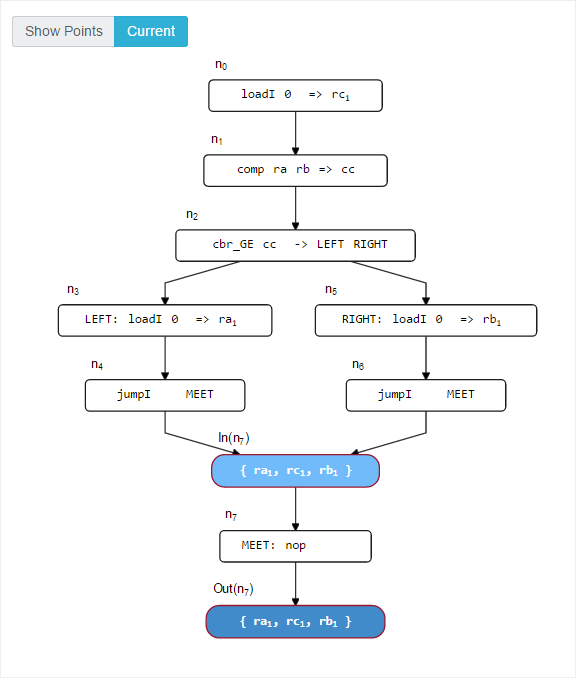
\includegraphics[width=\textwidth]{img/cfg-vis.png}
        %     \captionof{figure}{Control-Flow Graph Visualisation}\label{fig:cfg-vis}
        %   \end{minipage}
        %   \quad
        %   \begin{minipage}{.38\textwidth}
        %     \centering
        %     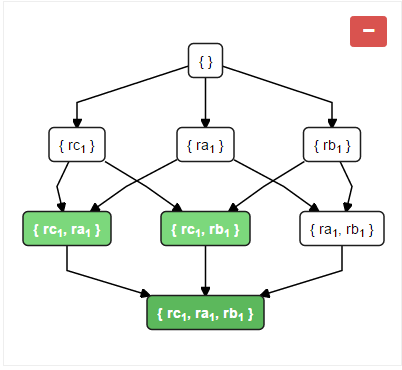
\includegraphics[width=\textwidth, trim=0 0 0 60]{img/lattice.png}
        %     \captionsetup{width=6cm, justification=centering}
        %     \captionof{figure}{Hasse Diagram Visualisation}\label{fig:lattice}
        %   \end{minipage}
        % \end{figure}


        To reduce clutter in the graph, the user has three options for
        displaying nodes: {\em current}, in which only the points
        relating to the current step are shown; {\em all}, in which
        every point is displayed; or {\em none}, in which only the
        nodes of the \gls{cfg} are shown. Fig. \ref{fig:cfg-vis} shows
        the \gls{cfg} in the {\em current} setting.

        \begin{wrapfigure}[22]{r}{8cm}
            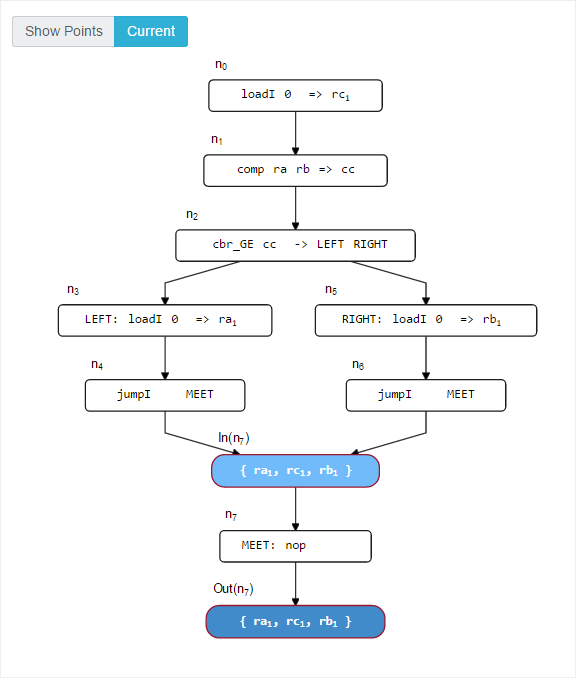
\includegraphics[width=9cm]{img/cfg-vis.png}
            \captionof{figure}{Control-Flow Graph Visualisation}\label{fig:cfg-vis}
        \end{wrapfigure}

        A system was devised to allow dynamic insertion and removal of
        points from the \gls{cfg}. In addition to automatically
        displaying nodes based on the settings described above, the
        component's \gls{api} can be used to add or remove specific
        points. This allows the tutorial examples to display the exact
        information required rather than relying on the simulation to
        process the desired nodes.

        As the user steps through a simulation, nodes and points in
        the \gls{cfg} are highlighted to visually relate them to
        actions occurring in other components. This is shown by
        fig. \ref{fig:cfg-vis}; the transfer function is reading
        information, shown in light blue, from In$(n_7)$ and modifying
        Out($n_7$), shown in dark blue.

        \subsection{Hasse Diagrams}

        \begin{wrapfigure}[12]{r}{6cm}
          \centering
          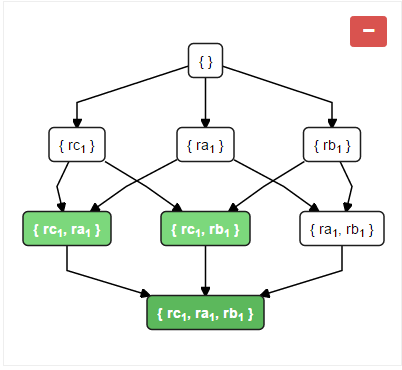
\includegraphics[width=7cm, trim=0 0 0 60]{img/lattice.png}
          \captionsetup{width=6cm, justification=centering}
          \captionof{figure}{Hasse Diagram Visualisation}\label{fig:lattice}
        \end{wrapfigure}

        The \gls{hassediagram} component is implemented using much the
        same system as the \gls{controlflowgraph}s. An SVG component
        is created, the nodes and edges are added to a dagre-d3 graph
        and the result is rendered to the screen.

        As the user steps through a simulation, nodes in the diagram
        are highlighted to visually relate them to actions occurring
        in other components -- during the meet phase, the sets being
        considered are highlighted in light green and the resulting
        set in dark green.

        \subsection{Table of Results}
        The table of results, which displays the set of values at each
        point, is simply a HTML table containing the required
        information. Various layouts were considered for this table,
        with the final design shown in fig. \ref{fig:tableofresults}.

        \begin{figure}[!ht]
          \centering
          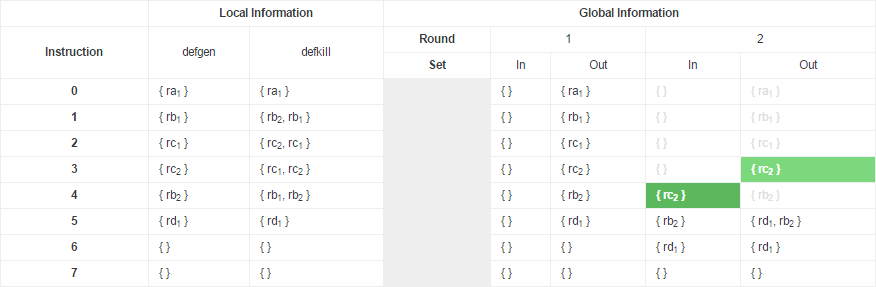
\includegraphics[width=\textwidth]{img/tableofresults.png}
          \caption{Current Table Layout}\label{fig:tableofresults}
        \end{figure}

        Cells in the table are highlighted to link them to other
        visual components. Any sets are read or modified, including
        local information, are higlighted in the table in each step of
        the simulation.

        This design could be improved by changing the layout of the
        table when viewed on small screen sizes. In the current layout
        the entire table becomes scrollable if it is too large for its
        canvas. Perhaps changing the table so that only the rounds
        become scrollable (see fig. \ref{fig:tablescroll})
        would improve its readability; however, the amount of time
        required to implement this was deemed better spent on
        implementing other functionality as the cases in which it is
        required are uncommon.

        \begin{figure}[!ht]
          \centering
          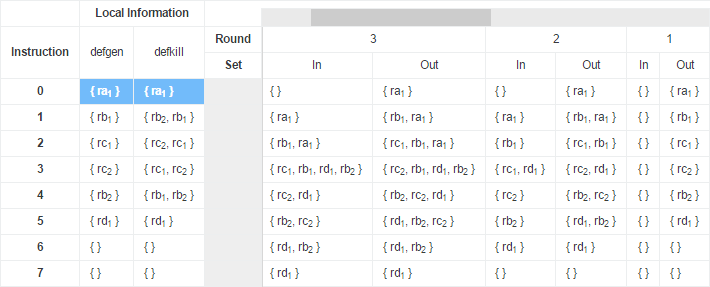
\includegraphics[width=13cm]{img/tablescroll.png}
          \caption{Alternate Table Layout with Scrollable Rounds}\label{fig:tablescroll}
        \end{figure}

        \subsection{Code Display}\label{sec:code-display}
        The code display handles displaying ILOC programs, with visual
        links to other components sharing the simulation. This is
        handled by a simple HTML table, as each ILOC instruction has a
        maximum of 7 fields: label, opcode, two sources, the
        $\rightarrow$ or $\Rightarrow$ symbol, and two
        targets. Aligning each token in the instruction allows the
        code to be read much more easily than if the raw text were
        displayed on screen. Fig. \ref{fig:code-display} shows the
        code display component.

        \begin{figure}[!ht]
          \hspace{2mm}
          \begin{minipage}{.43\textwidth}
            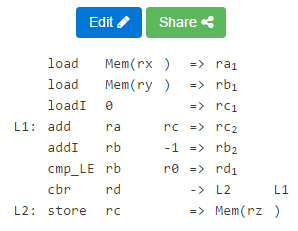
\includegraphics[width=\textwidth, trim=-15 -35 -15 0]{img/codedisplay.png}
            \captionsetup{width=\textwidth, justification=centering}
            \captionof{figure}{Default Code Display}\label{fig:code-display}
          \end{minipage}%
          \quad
          \begin{minipage}{.43\textwidth}
            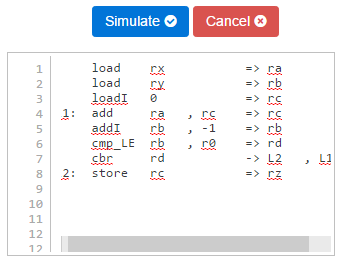
\includegraphics[width=\textwidth]{img/codeedit.png}
            \captionsetup{width=\textwidth, justification=centering}
            \captionof{figure}{Editing Code in the Simulator}\label{fig:code-edit}
          \end{minipage}
        \end{figure}

        \begin{figure}[!ht]
          \centering
          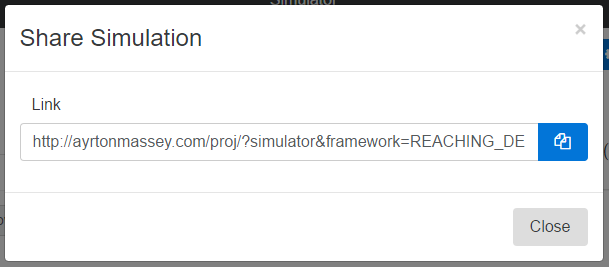
\includegraphics[width=8cm]{img/code-share.png}
          \caption{Share Code Dialog}\label{fig:code-share}
        \end{figure}

        In the simulator interface this view also handles editing or
        sharing code with others. Figures \ref{fig:code-edit} \&
        \ref{fig:code-share} show this in action. If the user enters
        invalid code an error message is displayed using line and
        column information obtained from PEGjs. Line numbers are
        displayed in the text area to help the user identify the
        source of the error; this functionality is provided by the
        jQuery Lined TextArea\cite{jquerylinedtextarea} plugin. The
        additional whitespace is added by the simulator to improve
        readability, but is not necessary.
        

    \section{Interactive Components}
    This section describes the implementation of the components which
    enable the user to interact with the system, including the choice
    of any libraries and frameworks and the changes that were made
    from the original design.
    
        \subsection{Simulator Controls}

        \begin{wrapfigure}[5]{r}{4cm}
          \centering
          
\includegraphics[width=4cm, trim=0 0 0 30]{img/simcontrols.png}
          \captionsetup{width=4cm, justification=centering}
          \caption{Simulator Controls}\label{fig:simcontrols}
        \end{wrapfigure}

        The simulator controls simply activate the playback functions
        in the simulator through its \gls{api}. The controls can be
        embedded in any other view, so whilst their main use is in the
        simulator interface it is also possible to include them in
        interactive tutorials or tests.

        \subsection{Questions}
        The {\tt QuestionView} class was designed to be adapted to as
        many situations as possible. Each question displays a number
        of possible answer, and has a variety of configuration
        options:

        \begin{itemize}
        \item The order in which answers should be presented (or
          shuffled).
        \item Whether a question allows multiple answer choices.
        \item Which answers should be revealed upon selecting an
          answer, if any.
        \item Which answers should be disabled upon selecting an
          answer, if any.
        \end{itemize}

        The question and its answers are rendered using the MathJax
        library to display mathematical formulae. Submitting a
        question reveals the nature of each answer (correct or
        incorrect) and marks those selected by the user. Answers may
        be assigned flavour text which is displayed upon selection to
        provide the user with instant, detailed feedback. Two example
        questions are shown in figures \ref{fig:multi-choice-q} \&
        \ref{fig:answered-q}

        \begin{figure}[!ht]
          \vspace{4mm}
          \hspace{2mm}
          \begin{minipage}{.43\textwidth}
            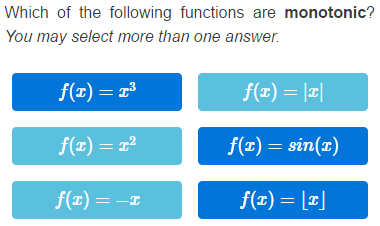
\includegraphics[width=\textwidth]{img/multiple-choice-q.png}
            \captionsetup{width=\textwidth, justification=centering}
            \captionof{figure}{A multiple-choice {\tt QuestionView}.}\label{fig:multi-choice-q}
          \end{minipage}%
          \quad
          \begin{minipage}{.53\textwidth}
            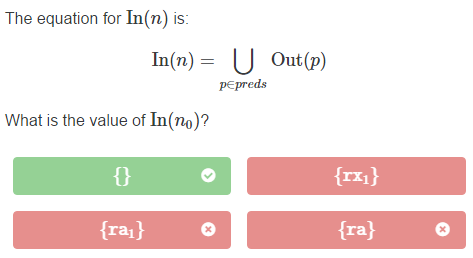
\includegraphics[width=\textwidth, trim=0 0 0 22]{img/answered-q.png}
            \captionsetup{width=\textwidth, justification=centering}
            \captionof{figure}{A {\tt QuestionView} after it has been submitted.}\label{fig:answered-q}
          \end{minipage}
        \end{figure}

        The highly configurable nature of the questions allows them to
        be re-used across the app. In {\tt TutorialView}s the answers
        are revealed immediately, whereas in {\tt TestView}s the test
        must be submitted before the user is given feedback. {\tt
          QuestionView}s are also used in the evaluation to collect
        categorization information from the user.

        Two callback functions can be passed to the {\tt QuestionView}
        to control the application's behaviour upon selecting an
        answer. This function can perform such actions as allowing the
        user to proceed by enabling navigation buttons, or altering
        neighbouring components to provide visual feedback.
            
    \pagebreak

    \section{User Interface}
    This section discusses the implemented user interface and
    describes any changes made from the proposed design. These changes
    and the use of any libraries and frameworks are justified.
    
        \subsection{Overview}
    
        The user interface, much like the visual components, is
        implemented using the {\tt View} model. The modular nature of
        the {\tt View} system means that it is easy to add or remove
        components or sections of the \gls{ui}. In the same way that the
        simulator and its visual components may be extracted from the
        rest of the system, the interactive learning components are
        independent of the \gls{dataflowanalysis} content. This would
        allow others to implement a similar system for other topics
        with only a small amount of work.

        A combination of the Bootstrap design framework, jQuery,
        Handlebars and MathJax libraries were used to produce the
        overall look and feel of the \gls{ui}. The latest development
        version of Bootstrap (v4-alpha-2) was used due to the addition
        of CSS {\tt flexbox} support -- whereas the current version
        (3.5.6) uses {\tt float}ing elements, {\tt flexbox} allows
        more control over the layout including more precise vertical
        alignment and scaling elements to fill their
        containers. Whilst similar layouts are possible in 3.5.6, they
        are often difficult or painful to achieve consistent behaviour
        across different web browsers.

        However, this increase in flexibility comes with some
        drawbacks. Load times of the application are reduced; though
        most of the JavaScript and CSS libraries are hosted using a
        \gls{cdn}, less common libraries such as this project's build
        of the Bootstrap alpha must be downloaded from the
        application's server. A \gls{cdn} would provide faster
        download speeds and enable the use of cached files if the user
        has visited other sites using the same libraries, whereas
        hosting them on the application server requires those
        libraries to be downloaded regardless of whether the user has
        already received them from another source.
    
        \subsection{Menu}

        \begin{figure}[!ht]
          \centering
          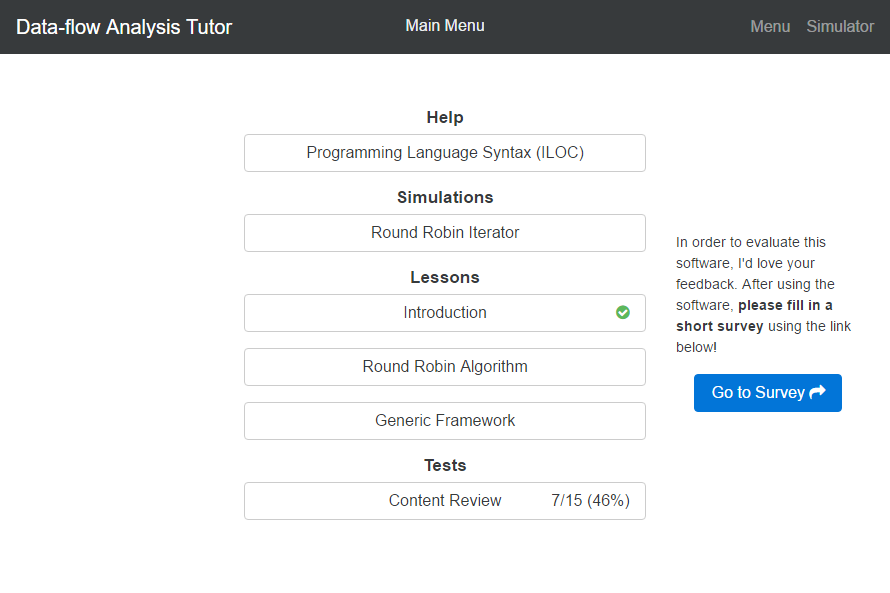
\includegraphics[width=\textwidth, trim=0 0 0 0]{img/menu.png}
          \captionsetup{width=\textwidth, justification=centering}
          \caption{The main menu of the application.}\label{fig:menus}
        \end{figure}

        The main menu is the first screen the user sees upon loading
        the app. The final design consists of a list of buttons which
        take the user to the corresponding view. This is similar to
        the original design but for a few key features: first, the
        description panel is missing -- this was a planned feature,
        but other parts of the software took priority and thus this
        was not implemented. Some of the content which would have
        appeared there, namely the test scores and the indicator that
        a lesson has been completed, have been moved inside the menu
        items themselves. The menu also lacks any icons to visually
        identify groups of items.

        One obvious improvement would be to include the planned
        description panel. It would also make sense to re-order the
        menu items such that the introductory lessons are at the top
        of the list; this would draw the users to those items and
        hopefully provide some guidance upon first use of the
        application. Finally, adding some visual cues such as images
        or icons would help the user quickly navigate the menu and
        break the monotony of the current design.

        \subsection{Simulation Interface}

        % \begin{figure}[!ht]
        %   \centering
        %   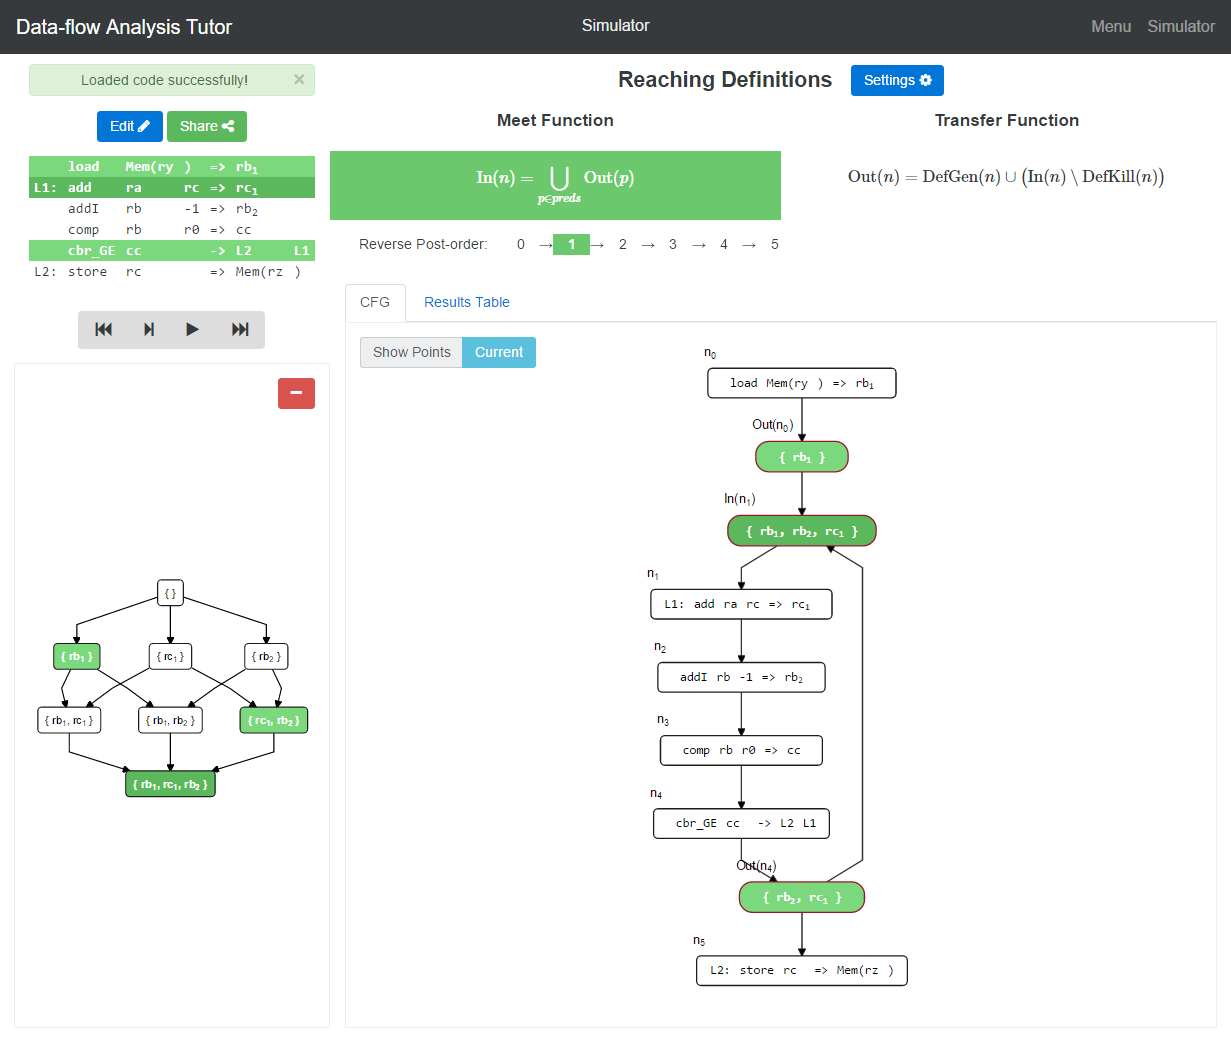
\includegraphics[width=\textwidth]{img/simulator2.png}
        %   \captionsetup{width=\textwidth, justification=centering}
        %   \caption{The simulator interface.}\label{fig:simulator}
        % \end{figure}

        The final simulation interface, shown in
        fig. \ref{fig:simulator}, is very similar to the original
        design. However, some changes had to be made to accommodate
        different screen sizes:
        
        \begin{itemize}
        \item The \gls{cfg} and table of results have been moved into
          separate tabs, as there was not enough room to display both
          simultaneously on small displays. This saves screen
          real-estate where it is needed, but wastes it where it is
          not -- the change could be improved by changing the layout
          to a side-by-side view on larger displays using JavaScript.
        \item The Hasse diagram component is collapsible, which
          increases the area available to the code display when
          simulating programs with many instructions. In cases where
          it is too large to be displayed it is replaced by a warning
          message.
        \item The simulation settings have been moved to a separate
          window. When the user clicks the ``Settings'' button is
          clicked a modal dialog appears, prompting them to change the
          configuration of the simulation. These settings were
          previously beside the \gls{dataflow} framework properties.
        \end{itemize}

        These are positive changes which increase the usability of the
        design for users of laptops or similarly sized devices. Other
        changes include the addition of the ``Share'' button (detailed
        in \S\ref{sec:code-display}) to allow students to share their
        programs and simulations with classmates or their professor,
        and the framework details now show the list of nodes in
        addition to the ordering in use. The use of colour and
        familiar icons draw the user to important features and clearly
        indicate the function of buttons and menus.

        An alternate design discussed in \S\ref{sec:design-simulator}
        proposed the use of a window system, which would allow the
        components to be dynamically rearranged or resized. However,
        the simulation interface lays out all of the available visual
        components in such a way that the maximum amount of
        information is conveyed without being too confusing or
        intimidating. The time which would have been spent developing
        the window system would likely not have been worth the effort,
        even with the availability of external libraries, given the
        strength of the implemented design.

        \begin{figure}[p]
          \centering
          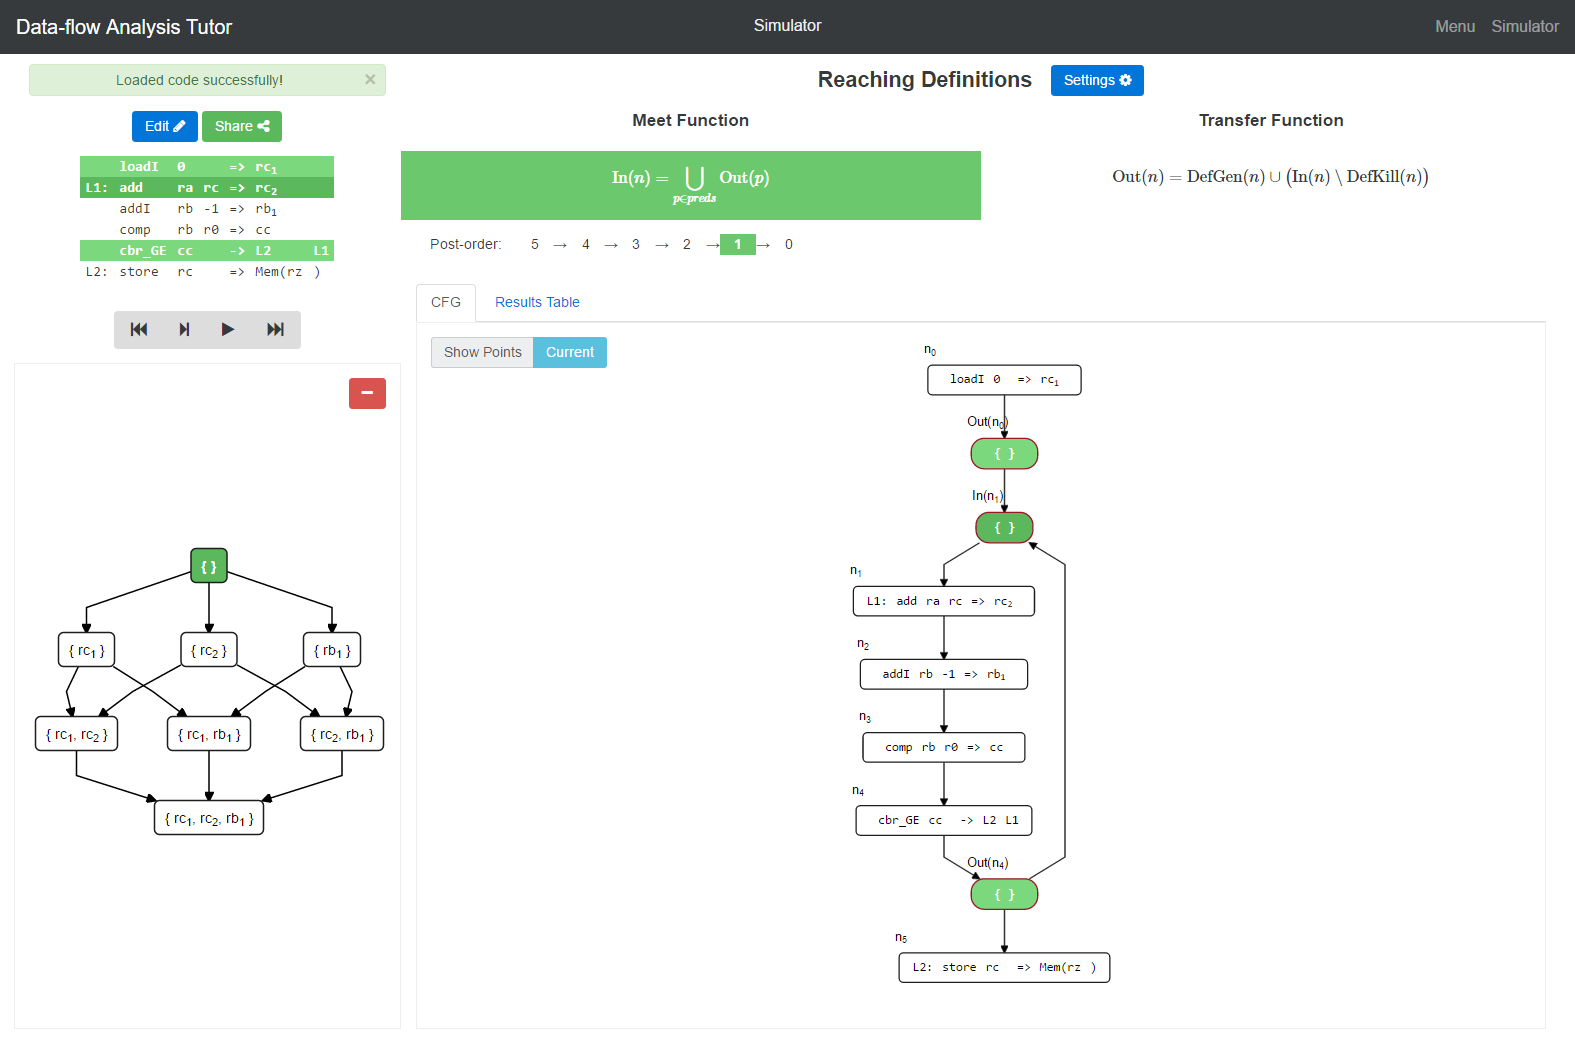
\includegraphics[width=\textheight, angle=-90]{img/simulator.png}
          \captionsetup{width=\textwidth, justification=centering}
          \caption{The simulator interface.}\label{fig:simulator}
        \end{figure}

        \subsection{Tutorial Interface}
        
        The tutorial interface is also very similar to the original
        design. The user follows a series of steps which present them
        with text descriptions and sometimes visual components. These
        steps are written in JavaScript and so are able to hook into
        the component or simulator \gls{api}s in order to manipulate
        them; for example, in fig. \ref{fig:tutorial} when the user
        selects the correct answer they are shown visual confirmation
        in the \gls{cfg} and table of results.

        The steps-as-functions system gives a lot of power to the
        developer at the cost of added complexity. Whilst this is
        great for complicated steps involving questions which trigger
        simulator events or manipulate visual components, many of the
        steps are simply a passage of text with some formulae. If the
        project were to be developed further or extended to other
        topics it would be useful to implement some kind of high-level
        description language for tutorials. Simple operations such as
        displaying text or a {\tt QuestionView} or advancing the
        simulation, could be written quite simply in this format. This
        follows the tried-and-true software enginering principle
        \gls{dry}.

        The current step implementation also has an unfortuate
        side-effect -- each step is dependent on the ones before it,
        so to navigate to a previous step the system must execute each
        of the preceding step functions (for example, to go from step
        38 to step 37 the system will reset and then execute steps
        1...37). When navigating forward through a tutorial, some
        steps taking slightly longer to load is barely
        noticeable. However, when navigating backward it becomes
        glaringly obvious, due to the cumulative effect of executing
        every step at once.

        The high-level description language mentioned above would
        enable some kind of state history system. Changes could be
        popped on and off a stack in order to navigate forward or
        backward, increasing the efficiency of navigation. This
        functionality would be abstracted away from the developer by
        the description language, removing any complexity faced when
        implementing this in the current system.

        \begin{figure}[!b]
          \centering
          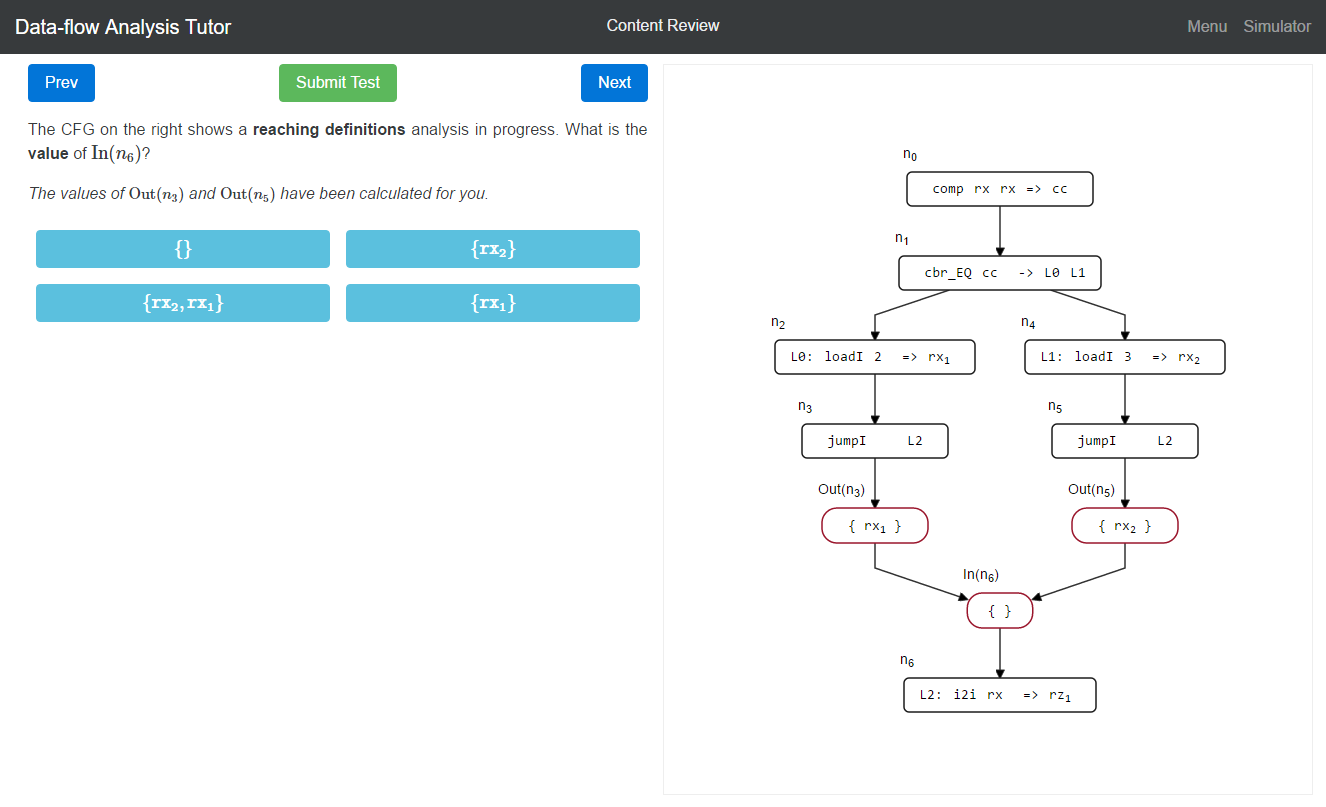
\includegraphics[width=\textwidth, trim=0 0 0 0]{img/test.png}
          \captionsetup{width=\textwidth, justification=centering}
          \caption{An interactive test.}\label{fig:testing}
          \vspace{-5mm}
        \end{figure}

        \begin{figure}[p]
          \centering
          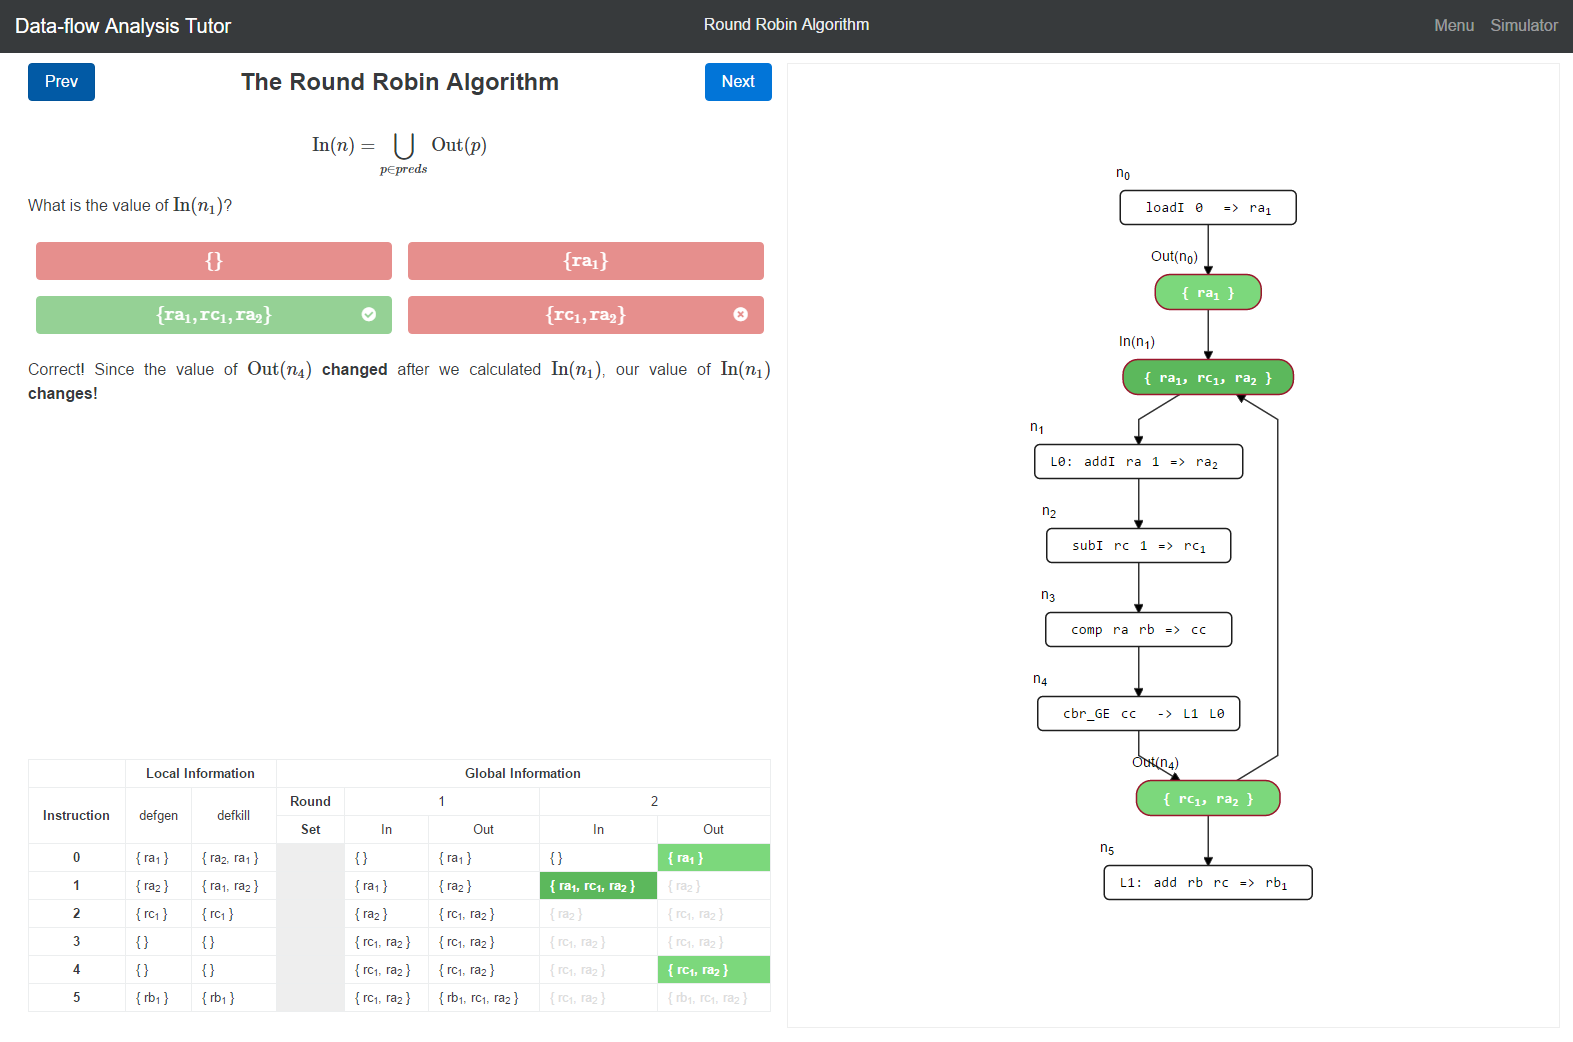
\includegraphics[width=\textheight, angle=-90]{img/lesson.png}
          \captionsetup{width=\textwidth, justification=centering}
          \caption{An interactive tutorial.}\label{fig:tutorial}
        \end{figure}

        \subsection{Testing Interface}

        The testing interface is a new feature not present in the
        original design. It was added for two reasons: first, to
        provide useful data in order to evaluate the project; second,
        to provide the user with a means of obtaining feedback about
        their learning progress.

        The design and implementation is an extension of the
        interactive tutorials. However, instead of suppling the code
        for each step of the program, a developer may supply text
        questions and answers with an optional function display any
        other components (such as a \gls{cfg}, as shown in fig
        \ref{fig:testing}). Unlike in the {\tt TutorialView}s,
        navigating to the previous question does not require every
        question to be re-initialized as each question is
        self-contained.

        Upon submission the user is shown some feedback and the
        correct answers are revealed, with icons to indicate which
        answers they picked to help them identify any mistakes they
        made. The feedback given is a simple overall score -- perhaps
        it would be more useful to provide a score breakdown by topic,
        to indicate which areas they need to improve upon. Some simple
        usability tweaks such as a progress indicator or a dialog to
        confirm whether the user would like to submit the test would
        not go amiss.


%%%%%%%%%%%%%%%%%%%%%%%%%%%%%%%%%%%%%%%
\chapter{Evaluation}
This chapter describes the evaluation methodology for the project,
followed by a critical analysis of the design and implementation of
the system and suggestions for future development. The chapter
concludes with an assessment of the success or failure of the project
as a whole.

    \section{Introduction}
    The goal of this project was to create an interactive system to
    teach students the basic principles of \gls{dataflowanalysis} in
    compilers. The final system took the form the form of an online
    learning platform, containing a \gls{dataflowanalysis} simulator
    and a series of interactive tutorials.

    To determine whether the final product meets the original aim of
    the project, there are three main points against which it should
    be evaluated:

    \begin{itemize}
    \item Interactions with the system, to analyse the users'
      engagement with the platform;
    \item Achievement of learning outcomes by the participants, in
      order to assess its validity as a learning platform; and
    \item Feedback from the participants, to determine whether it is a
      useful tool for the intended audience.
    \end{itemize}

    The following sections present a thorough evaluation of the
    system against these three objectives.

    \section{Method}

    The intended audience of the project is primarily students of the
    \gls{copt} course. However, the number of students available is
    limited; the course has around 30 registered students and
    anecdotal evidence shows that around 10 of those regularly attend
    class. In order to collect a suitable amount of data to perform an
    evaluation the net must be widened to include participants from
    outside the course, perhaps including those with prior experience
    in STEM subjects or students in general. The aim was to obtain
    around 30 responses, as this is generally seen as a reasonable
    sample size in statistical analysis.

    Evaluating the system requires the collection of data and
    supporting evidence from which conclusions may be drawn. There are
    a number of ways in which this data could be collected; for
    example, in-person evaluations may be performed and the sessions
    recorded. These recordings would then be analysed to obtain
    feedback. However, this method presents some issues: firstly, the
    participant may feel pressured to give a positive response in
    order to please the person conducting the evaluation. Second,
    whilst observing the participant would provide valuable insight
    into how participants use the application, it is very time
    consuming and difficult to find willing participants given the
    required time investment. To obtain the desired 30 responses, a
    more efficient method of data collection was required.

    Two possible methods which would enable remote participation
    involve collecting usage information or distributing an online
    survey to gather feedback. These methods are useful but can be
    unreliable; when collecting usage information if the user has
    JavaScript disabled or their internet connection drops then loss
    of data could occur. It is also difficult to determine whether
    respondents to an online survey have actually used the software
    without witnessing them do so.

    The most effective solution would therefore involve a mixture of
    all three methods: performing a few evaluation sessions in person
    would ensure that the methodology was sound and that the automated
    data collection functioned as intended, whilst enabling
    participants to complete the evaluation in their own time and
    removing the need for an assessor to be present. This also
    alleviates any pressure the participant may feel to provide a
    positive response.

    This was the method chosen to evaluate the project: participants
    were given a link to the application and usage information was
    collected with their consent. Upon accessing the application for
    the first time, users were asked two questions in order to
    categorize them (see \S\ref{sec:demographics}). A link in the
    application gave users the option to participate in a feedback
    survey. Three in-person evaluation sessions were held: two
    one-to-one sessions in order to validate the evaluation method
    itself, and one in-class session with the \gls{copt}
    students. 

    These sessions went well and thus an invitation was extended to
    the following sources:

    \begin{itemize}
    \item The remaining \gls{copt} students who did not attend the
      in-class session;
    \item Friends and family through my personal Facebook feed;
    \item Members of the ``Informatics -- Class of 2016 --
      University of Edinburgh'' and ``Informatics -- University of
      Edinburgh'' Facebook pages;
    \item Students of the Compilers courses at the Universities of
      Bristol, Birmingham, Durham, Oxford, Manchester, Warwick,
      Imperial College London and UCL, whose organisers' e-mail
      addresses were publicly available; and
    \item Members of the /r/compilers, /r/computerscience and
      /r/webdev communities on Reddit\cite{reddit}.
    \end{itemize}

    This should encourage participants from a wide range of
    backgrounds, including those with prior experience with or an
    interest in studying \gls{dataflowanalysis}, those with knowledge
    of similar material such as Computer Science and STEM students,
    developers of web applications who should be familiar with
    \gls{ux} and \gls{ui} design, and those completely unrelated to
    any technical fields.

    All participants were presented with the same version of the
    software and were encouraged to be truthful and honest with their
    feedback.

        \subsection{Usage Data}
        To collect usage information, the use of some tracking system
        was required. A variety of web platforms exist for this
        purpose including Google Analytics and Piwik. However, these
        platforms are intended for large-scale data collection and as
        such are not suited for the fine-grained analysis necessary in
        the evaluation of this project. For example, it is not
        possible to link tracked events to specific users or view a
        complete list of triggered events using Google
        Analytics. Furthermore, extended use of these platforms often
        comes at significant financial cost. It is also important to
        consider the ethical issues that may arise from sharing usage
        data with companies like Google; using such a platform would
        require a much deeper discussion around user privacy and use
        of the data for financial gain.

        Developing a custom event-tracking \gls{api} would allow full
        control of the data collected both in terms of accessing the
        raw data and maintaining user privacy. The data model used in
        this \gls{api} must be able to store the following on a
        per-user basis:

        \begin{itemize}
        \item Page views;
        \item Button clicks and interactions with components;
        \item Page load times; and
        \item Question attempts and overall scores.
        \end{itemize}

        This data can be collected using an API with a single
        endpoint\footnote{An endpoint is a URL at which a particular
          API service may be accessed, e.g. \url{api.com/users/} may
          provide access to user data}, based on the Google Analytics
        event model. Each {\tt event} record has the following fields:

        \begin{itemize}
        \item A {\tt tracking token} used to group events by user;
        \item A {\tt type} such as page view or button click;
        \item The {\tt datetime} at which the event occurred; and
        \item Four levels of categorization: {\tt category}, {\tt
            action}, {\tt label}, and {\tt value}. Each field can be
          used to group similar events and store values such as
          question scores or which element was clicked. The actual
          content of these fields does not matter as long as the
          grouping is consistent.
        \end{itemize}

        The tracking token is generated when the user first visits the
        page and persists across visits to the site. Storing this
        token enables analysis of how a user's actions affect their
        achievement of learning outcomes, such as whether completing a
        given tutorial or using a simulator component increases
        question scores in the related topic. It would be possible to
        determine which elements of the software users find difficult
        to understand based on their interactions with each component.

        This design was implemented in Python using
        \gls{drf}\cite{drf}, due to the ease with which one may
        develop a simple web \gls{api}. This application was hosted on
        an Apache server using the {\tt mod\textunderscore{}wsgi}
        module. The \gls{api} receives events as \gls{json} data and
        stores them in a PostgreSQL database hosted on the same
        server. A small JavaScript library was written to generate
        identification tokens and send user events to the \gls{api}.

        All of the data sent to the API is completely anonymous; the
        tracking token is randomly generated and exists only to tie
        records to a given session. In addition to the events outlined
        above, the application sends the user's categorization answers
        to the \gls{api} to provide context to the data collected.

        \subsection{Feedback Survey}
        After using the software, participants had the option to fill
        out a short evaluation survey. This survey was produced using
        Google Forms\cite{googleforms} because of its flexibility and
        low risk regarding loss of data.

        The first page of the form, which requests the same
        categorization information as the application, is
        automatically filled if the user follows the link to the
        survey from the application's main menu. This reduces the
        amount of time users must spend filling out the survey and
        increases consistency between the data collected via the
        \gls{api} and the survey.

        Following the example set by Mustafa\cite{mustafa2010} (see
        \S\ref{sec:mustafa-simulator}), the survey consists of a
        number of \gls{likertscale} questions ranging from ``Strongly
        Agree'' to ``Strongly Disagree''. Partipants were required to
        select a response to each Likert item, but were given a ``No
        Response'' option instead of the usual ``Neutral'' response
        which allowed them to explicitly indicate that they did not
        wish to respond or that they had no strong feelings one way or
        another. This provided context as to why participants did not
        respond to a particular item, ensuring that they did not
        accidentally miss a question.

        More information about the content of the survey can be found
        throughout the remainder of this chapter.

    \section{Demographics}\label{sec:demographics}
    
    During the two-week evaluation period 184 unique users visited the
    application, 37 of whom used the software for more than 5
    minutes. The data used throughout the rest of this chapter has
    been culled to those 37 users who spent more than 5 minutes with
    the software.

    \begin{wrapfigure}[11]{r}{.38\textwidth}
      \vspace{-12mm}
        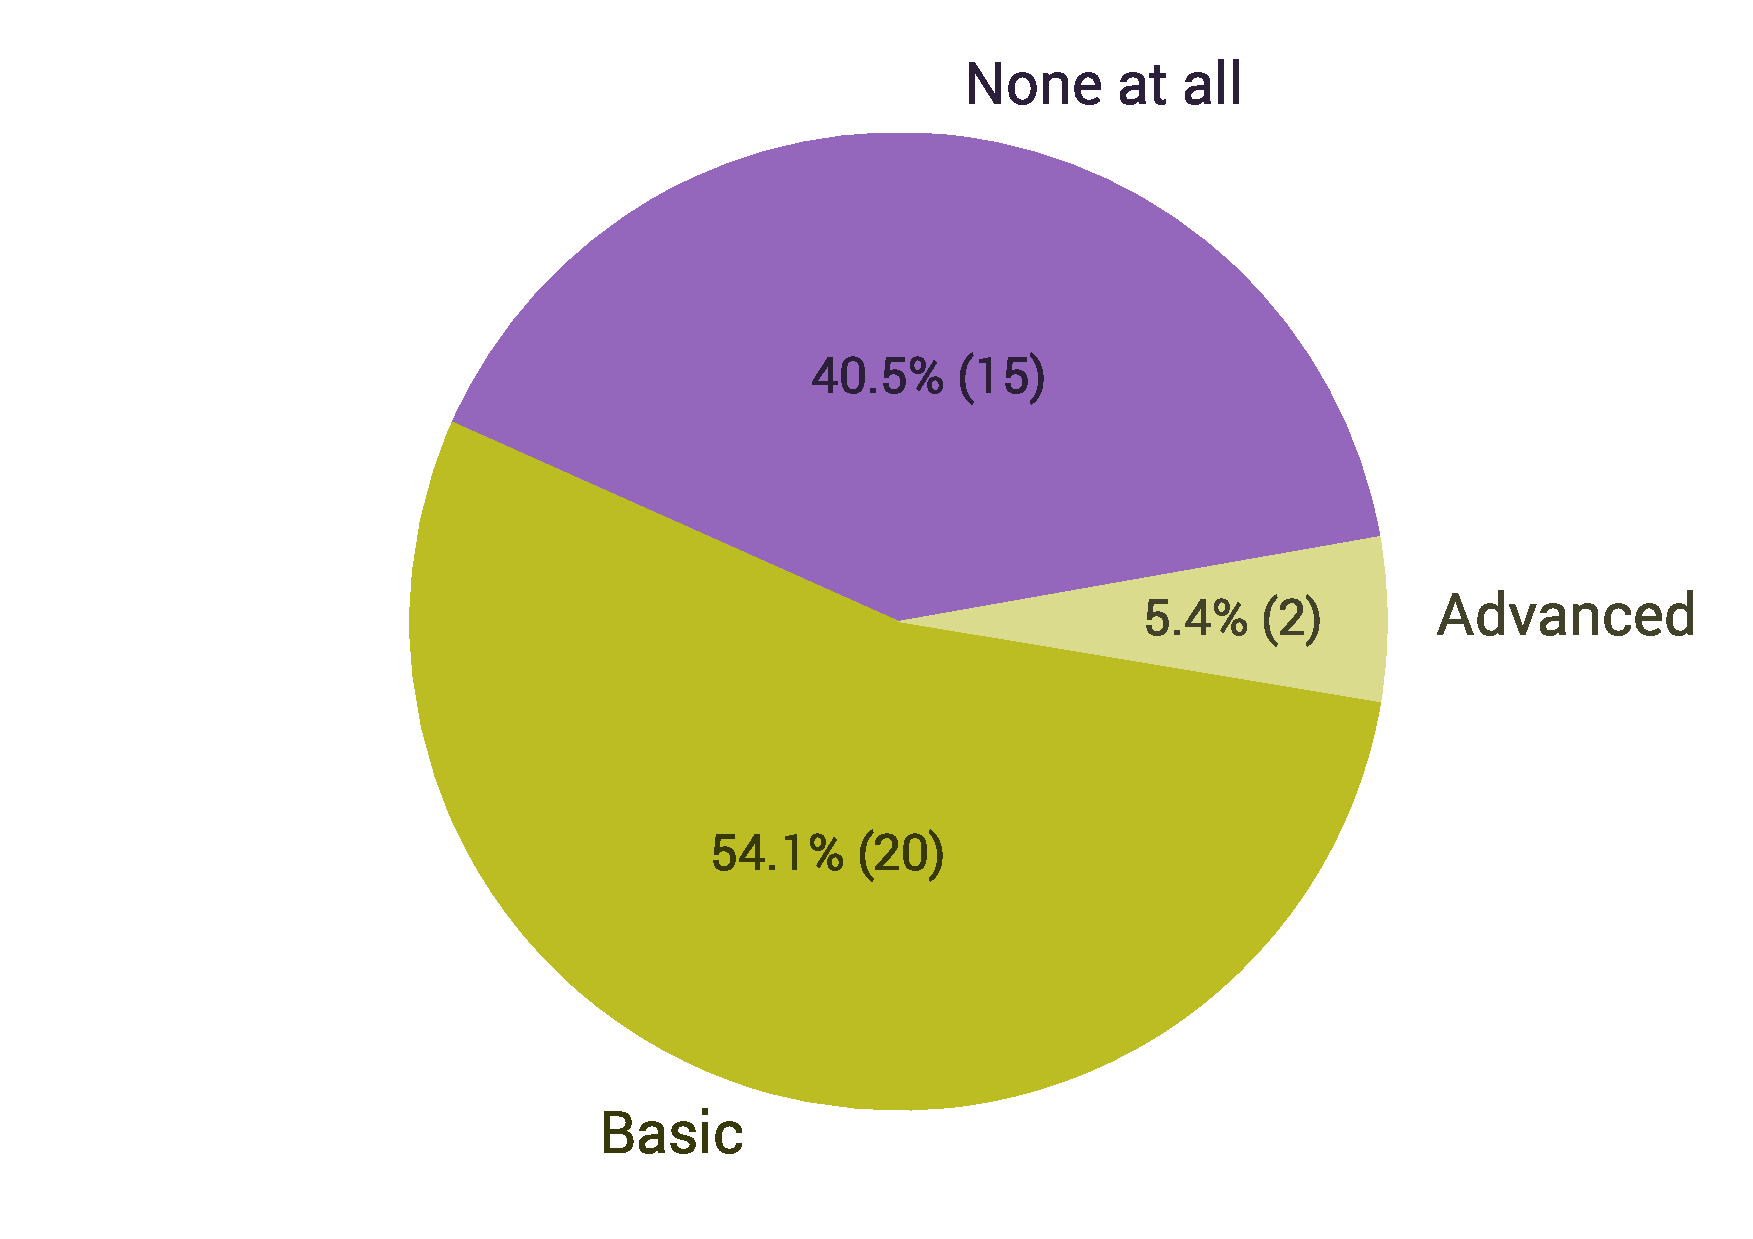
\includegraphics[width=.40\textwidth, trim=150 0 100 0]{img/experience_pie.pdf}
        \captionsetup{width=.38\textwidth, justification=centering}
        \caption{Distribution of User Subject Experience}\label{fig:demo-q1}
    \end{wrapfigure}

    Upon accessing the application for the first time, users were
    presented with two questions in order to categorize them based on
    their interest and experience in \gls{dataflowanalysis}. The first
    question asked them to rate their level of experience given the
    following options:

    \begin{itemize}
    \item None at all
    \item Basic
    \item Advanced
    \end{itemize}

    A summary of the response to the this question is shown in
    fig. \ref{fig:demo-q1}.

    The second question asked them to describe their academic
    background by selecting from a number of choices. These options
    were then ranked in the following order, by their relation to
    \gls{dataflowanalysis}:
    
    \begin{enumerate}
      \item I am a member of the COPT course (UoE only)
      \item I have studied Computer Science at degree level.
      \item I have studied a STEM subject at degree level.
      \item I am a student.
      \item (None of the above)
    \end{enumerate}

    Each user has been grouped by the highest-ranked option they
    selected; the distribution of these groups is shown in
    fig. \ref{fig:demo-q2}.

    \begin{figure}[!hb]
      \centering
      \captionsetup{width=\textwidth, justification=centering}
      \caption{Distribution of User Academic Experience}\label{fig:demo-q2}
      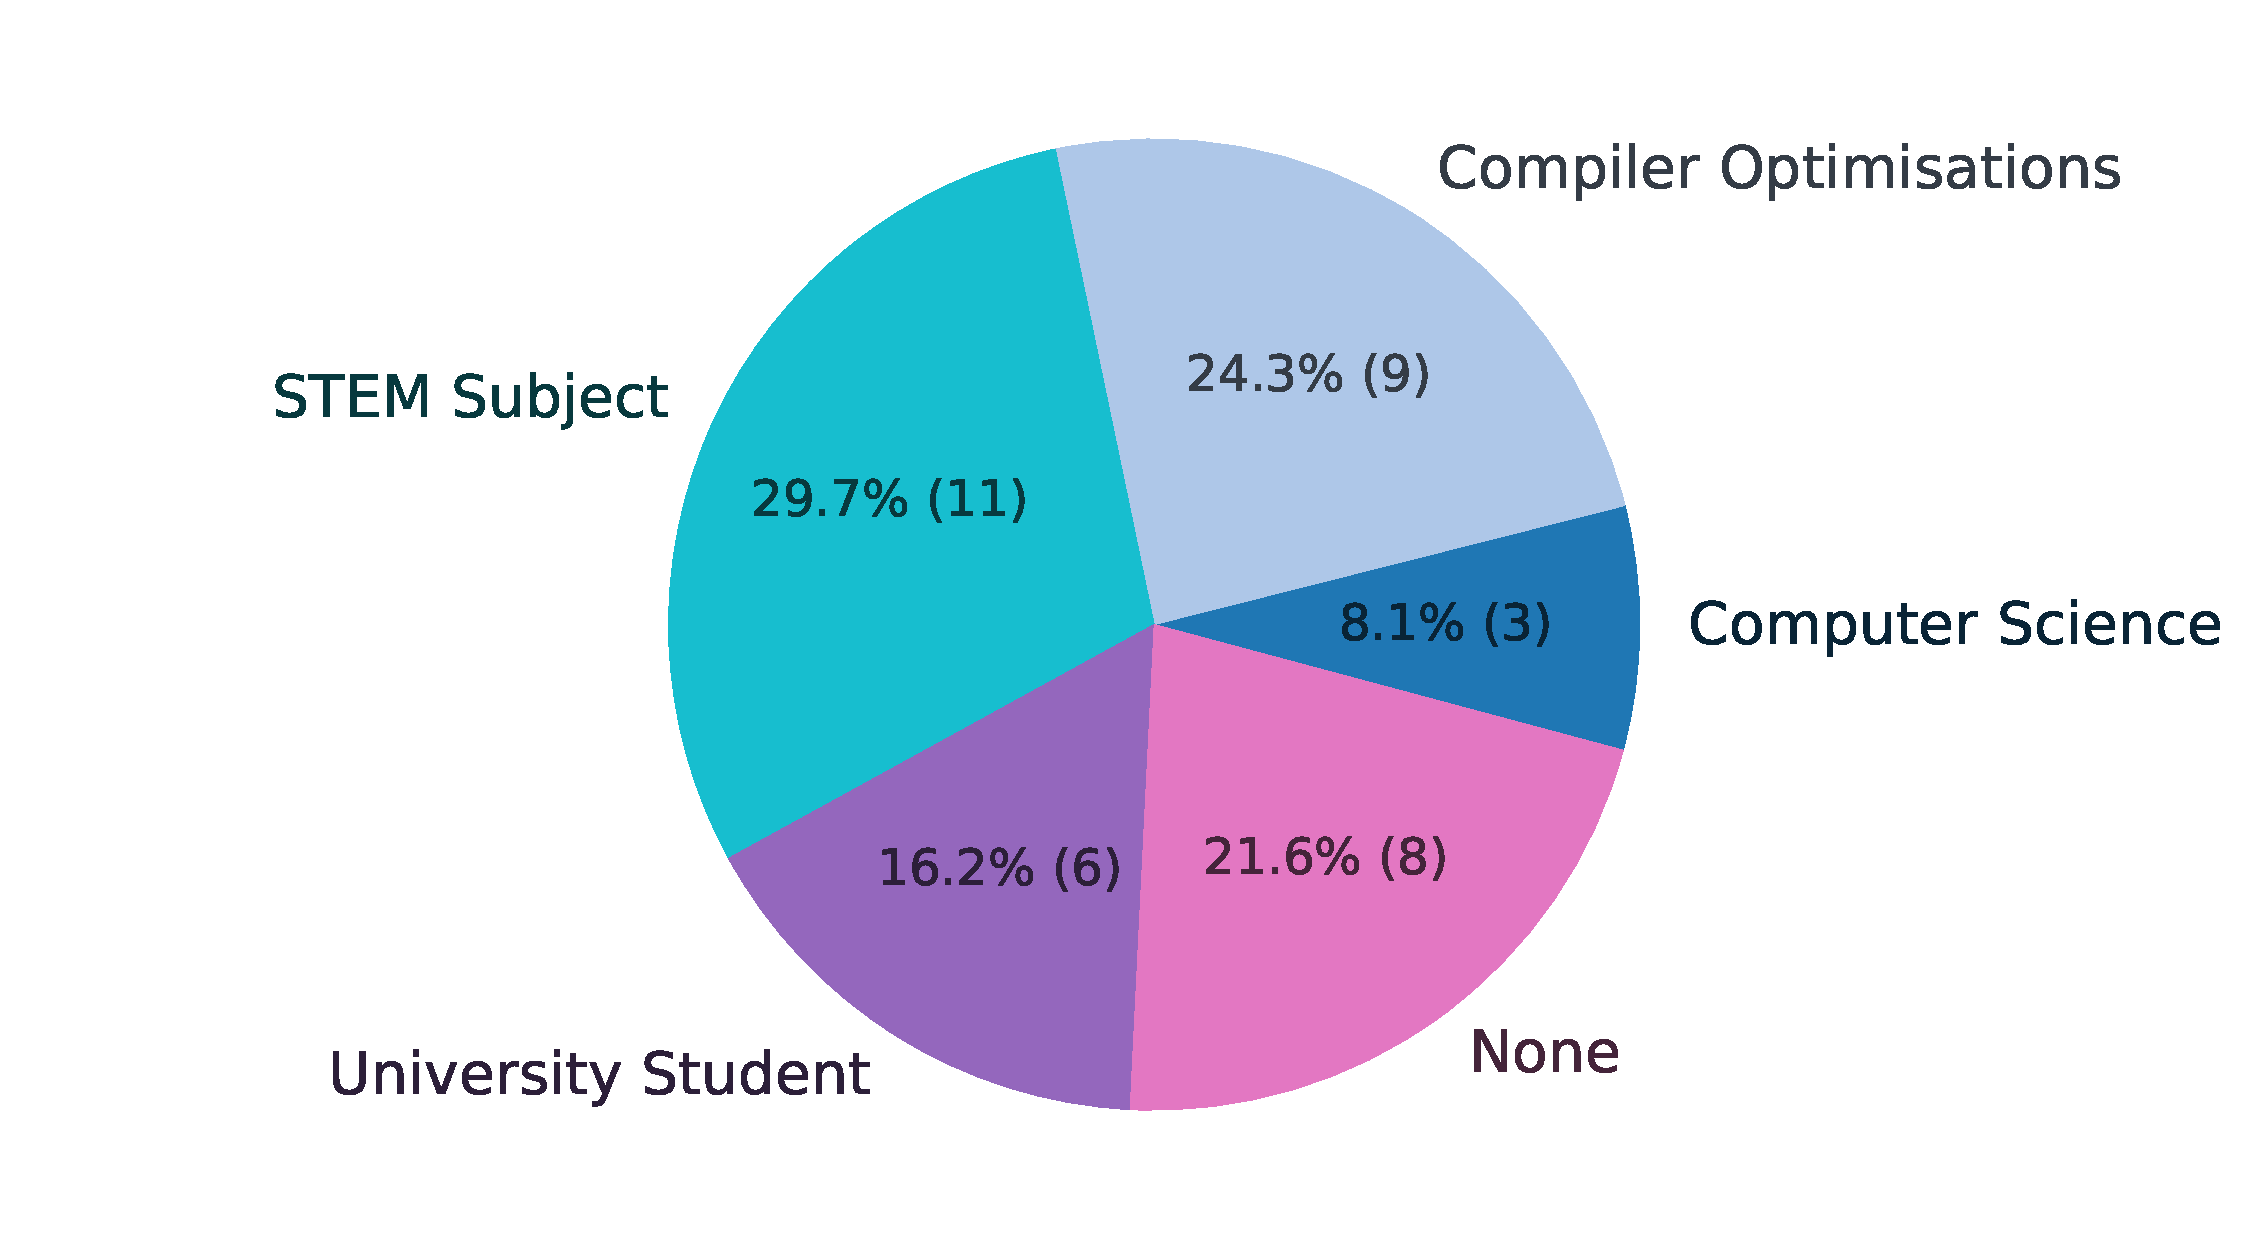
\includegraphics[width=0.9\textwidth, trim=40 200 0 0]{img/background_pie.pdf}
    \end{figure}

    These figures are quite positive. The participants come from a
    wide range of academic backgrounds and have a good mixture of
    prior experience with the topic. Although the number of
    participants is only 20\% of the total number of unique visitors,
    the low retention rate may be attributed to a number of factors:

    \begin{itemize}
    \item Users who visited the application but did not have time to
      invest in evaluating it;
    \item Users who visited the site but did not want to participate
      in the evaluation;
    \item Users who were not interested in the content; and
    \item Web crawlers visiting the page.
    \end{itemize}

    For an application targeting a relatively niche subject, a 20\%
    retention rate seems quite reasonable and does not indicate any
    particular flaws with the system.

    \section{Critical Analysis}
    In this section I will attempt to draw conclusions about the
    system by analysing usage data collected over the evaluation
    period.

    \subsection{Time Spent}

    As mentioned in \S\ref{sec:demographics}, a total of 37
    participants used the application for more than 5 minutes. This
    information was calculated by examining blocks of events triggered
    by each user. A {\em block} is defined as a sequence of events in
    which there is less than a 10-minute gap between consecutive
    records; the duration of these blocks is summed to produce an
    estimate of time spent during the two-week evaluation
    period. Fig. \ref{fig:time-hist} shows the distribution of time
    spent by those 37 participants, categorized by their experience
    with the subject.

    From this data, we can draw a number of conclusions: first, that a
    significant amount of users found the software engaging or at
    least of some use -- more than half of the participants used the
    software for more than 15 minutes, with at least one individual
    using it for over two hours. Of the users who stayed for more than
    15 minutes, most tended to invest a significant amount of time
    into using the application. This is promising -- anecdotally, I
    have noticed that project evaluation participants tend to quickly
    scan through the available features and then fill in the survey
    without spending enough time to thoroughly evaluate the
    application; however, the majority of users in this evaluation
    seem to have shown genuine interest in the system and its content.

    Second, it appears that the more experience a user has, the less
    time they are likely to spend using the application. Users who
    considered themselved ``Advanced'' in the topic spent the least
    time with the software, whilst those with no experience spent the
    most. This could indicate that the content presented by the system
    is too simple or that it re-treads too much ground covered by
    other sources such as lectures or textbooks.

    \begin{figure}[!hb]
      \centering
      \vspace{-2mm}
      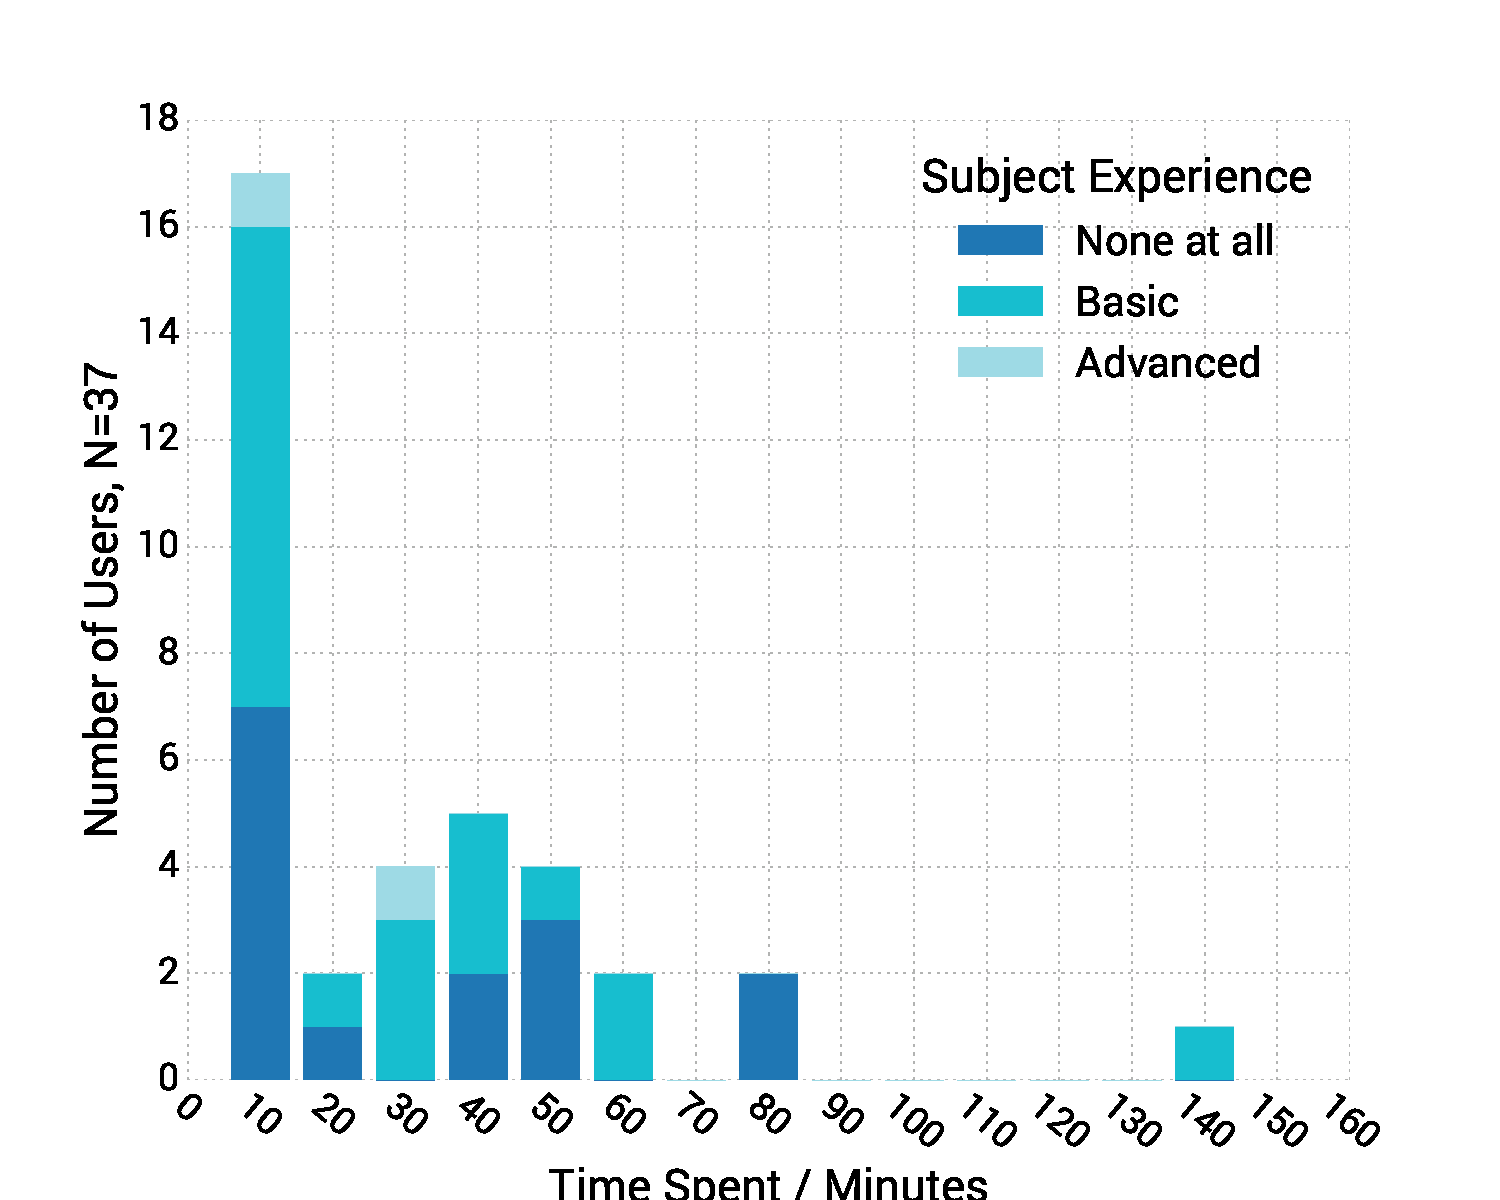
\includegraphics[width=.80\textwidth, trim=0 20 0 45, clip]{img/time_distribution.pdf}
      \captionsetup{width=\textwidth, justification=centering}
      \caption{Distribution of Time Spent Using the Application per User}\label{fig:time-hist}
    \end{figure}

    Users were encouraged to continue using the software after they
    had participated in the evaluation and completed the feedback
    survey. Fig \ref{fig:days-spent} shows how often users returned to
    the site. Although the majority of users only visited on the day
    they evaluated the application, 24\% returned to the application
    more than once, and one user in particular visited on 9 separate
    days.

    \begin{figure}[!htb]
      \centering
      % \vspace{-5mm}
      \captionsetup{width=\textwidth, justification=centering}
      \caption{Distribution of Returning Users}\label{fig:days-spent}
      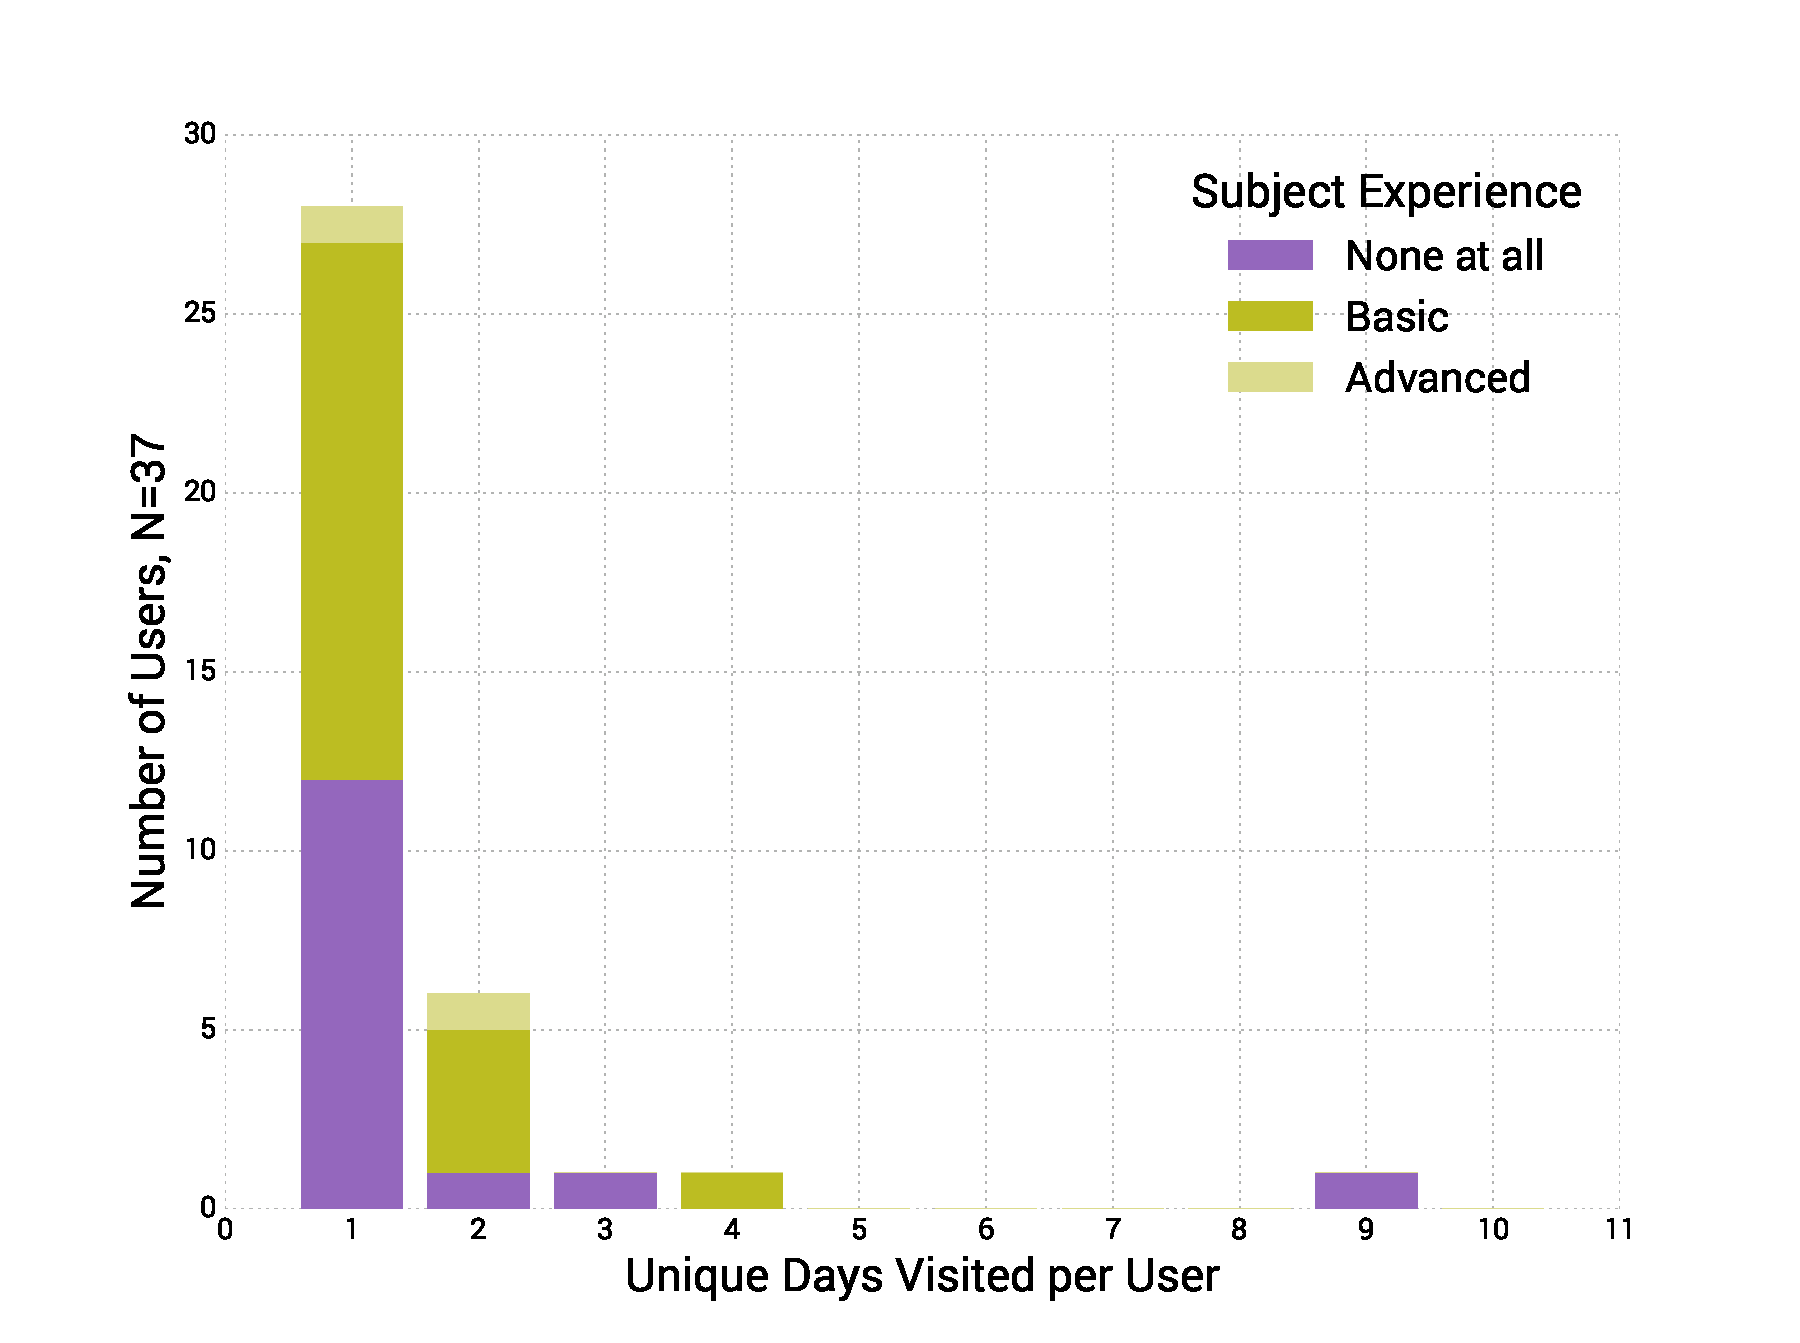
\includegraphics[width=.80\textwidth, trim=0 120 0 25]{img/unique_days.pdf}
    \end{figure}

    \subsection{Lessons Completed}

    \begin{wrapfigure}[21]{r}{6cm}
      \centering
      \vspace{-18mm}
      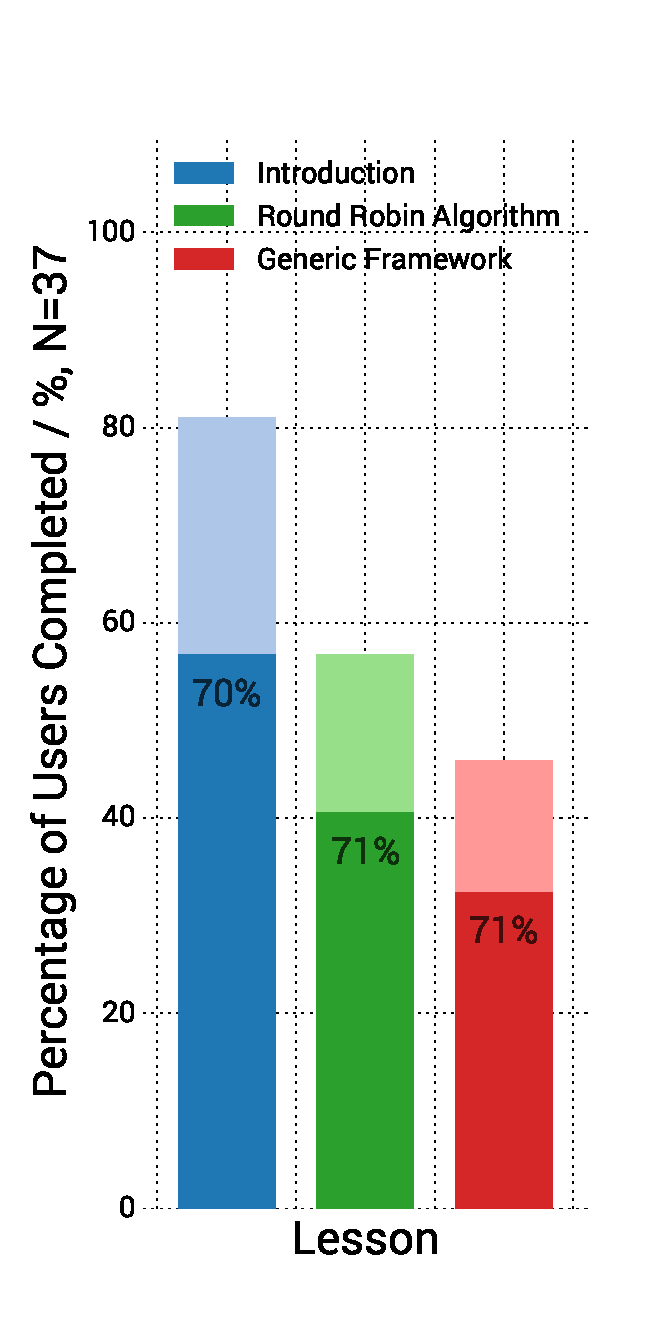
\includegraphics[width=5cm, trim=15 35 35 45, clip]{img/lessons.pdf}
      \captionsetup{width=5cm, justification=centering}
      \caption{Lessons Completed by Participants}\label{fig:lessons-complete}
    \end{wrapfigure}

    Fig. \ref{fig:lessons-complete} shows the number of lessons
    attempted versus the number of lessons completed. The pale bars
    represent the percentage of people who attempted each lesson,
    whilst the darker bars represent the percentage of people who
    completed them. The numbers in each bar represent the proportion
    of those who started the lesson and subsequently completed it.

    The results show that most users attempted the introductory
    lesson, with participation decreasing moderately for subsequent
    lessons. This is as expected; during the in-person evaluations
    participants were recommended to at least complete the
    introductory lesson. However, the participation rate for
    subsequent lessons is excellent -- above 50\% of the participants
    voluntarily attempted the second lesson, and 45\% attempted the
    third.

    The completion rate is fairly consistent, at around 70\%. Each
    lesson requires some form of active participation in order to
    continue, indicating that the lessons kept users engaged
    throughout.

    In the feedback survey, 22 of 28 users said that they had used the
    tutorial system. These users were asked to provide reasons why
    they did or did not complete a lesson after starting it. The
    feedback from these questions is shown in figures
    \ref{fig:lesson-stay} \& \ref{fig:lesson-leave}.

    \begin{figure}[!htb]
      \centering
      \captionsetup{width=\textwidth, justification=centering}
      \caption{Reasons Provided for Completing Lessons (N=28)}\label{fig:lesson-stay}
      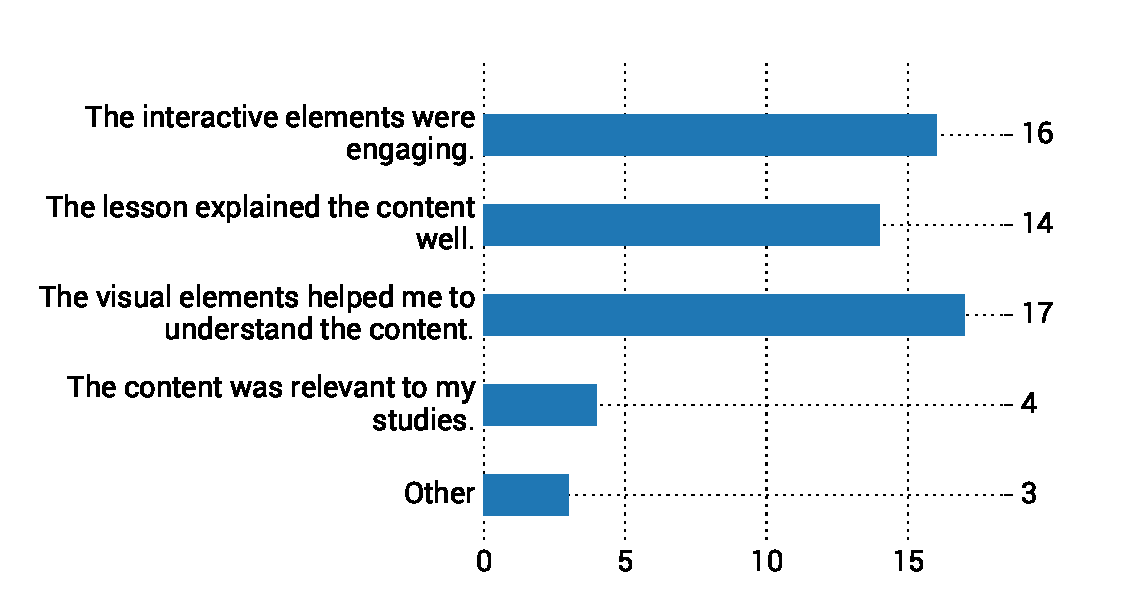
\includegraphics[width=\textwidth, trim=0 10 0 45, clip]{img/lesson_staying.pdf}
    \end{figure}

    The majority of users credited the interactive and visual elements
    as reasons for completing lessons. Half of the responses to the
    survey said that the lessons explained the content well, but only
    14\% said that it was relevant to their studies. This may be due
    to the low participation by \gls{copt} students, but in any case
    implies that perhaps more care should be taken when considering
    what material to cover.

    Of the three ``Other'' responses, two were joke comments, but the
    third was particularly revealing: a user responded that being able
    to select from existing answers, rather than having to type in
    formulae, was ``a win''. Online assessment platforms often require
    users to type in a textual representation of some formulae, but
    marking of these answers via a computer is difficult and is prone
    to false negatives. I had considered including some text-answer
    questions, but decided against it for this reason.

    \begin{figure}[!htb]
      \centering
      \vspace{-2mm}
      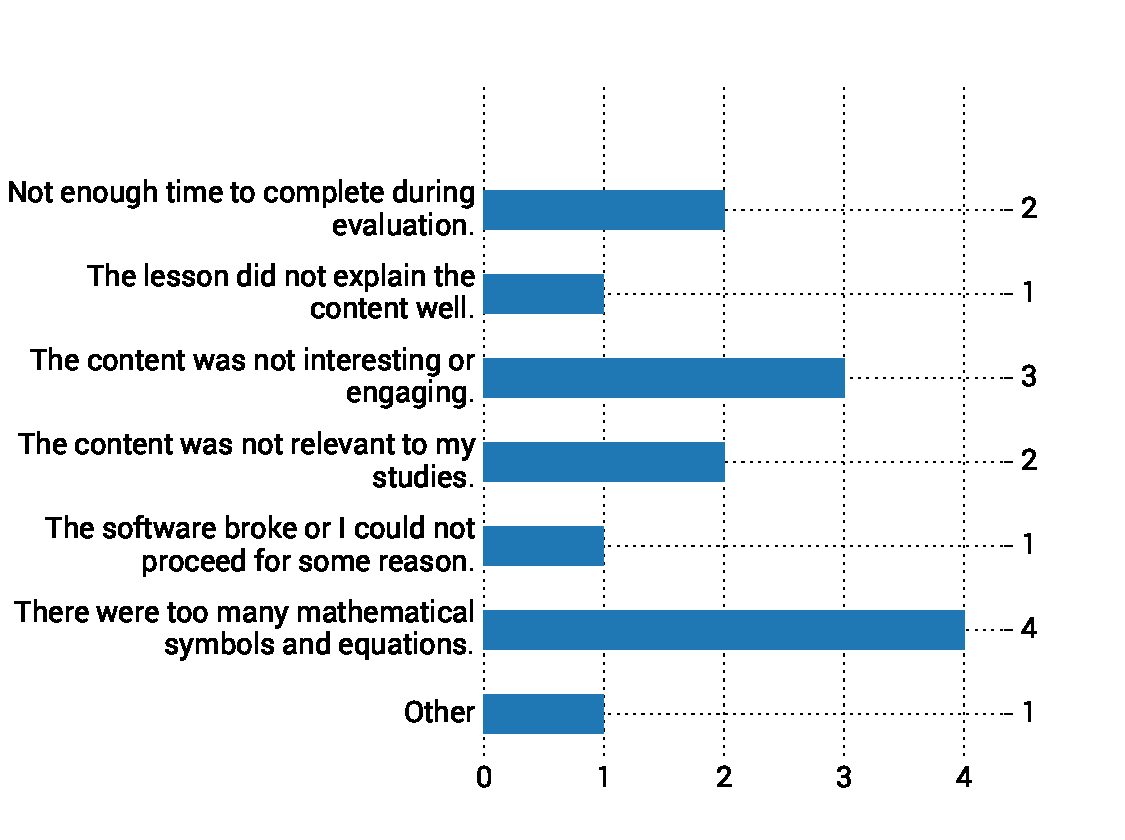
\includegraphics[width=\textwidth, trim=0 20 0 75, clip]{img/lesson_leaving.pdf}
      \captionsetup{width=\textwidth, justification=centering}
      \caption{Reasons Provided for Abandoning Lessons}\label{fig:lesson-stay}
    \end{figure}

    Of those who abandoned a lesson, the majority opinion was that
    there were too many mathematical formulae involved. This is true
    of the last lesson in the series, but unfortunately this is
    unavoidable as a large portion of the material is based in
    mathematical proof. However, this is certainly a point to consider
    when designing the content for learning platforms in the future,
    and efforts could be made to simplify the information presented by
    this system.

    \subsection{Achievement of Learning Outcomes}
    Participants were given the option to take a short content review
    test (consisting of 10 questions) during their use of the app. Of
    the 37 participants, 16 of them made a total of 20 attempts. I
    have analysed the scores achieved in each attempt in order to
    assess the participants' achievement of learning outcomes; this
    graph is shown in fig. \ref{fig:question-answers}.

    \begin{figure}[!tb]
      \centering
      \vspace{-6mm}
      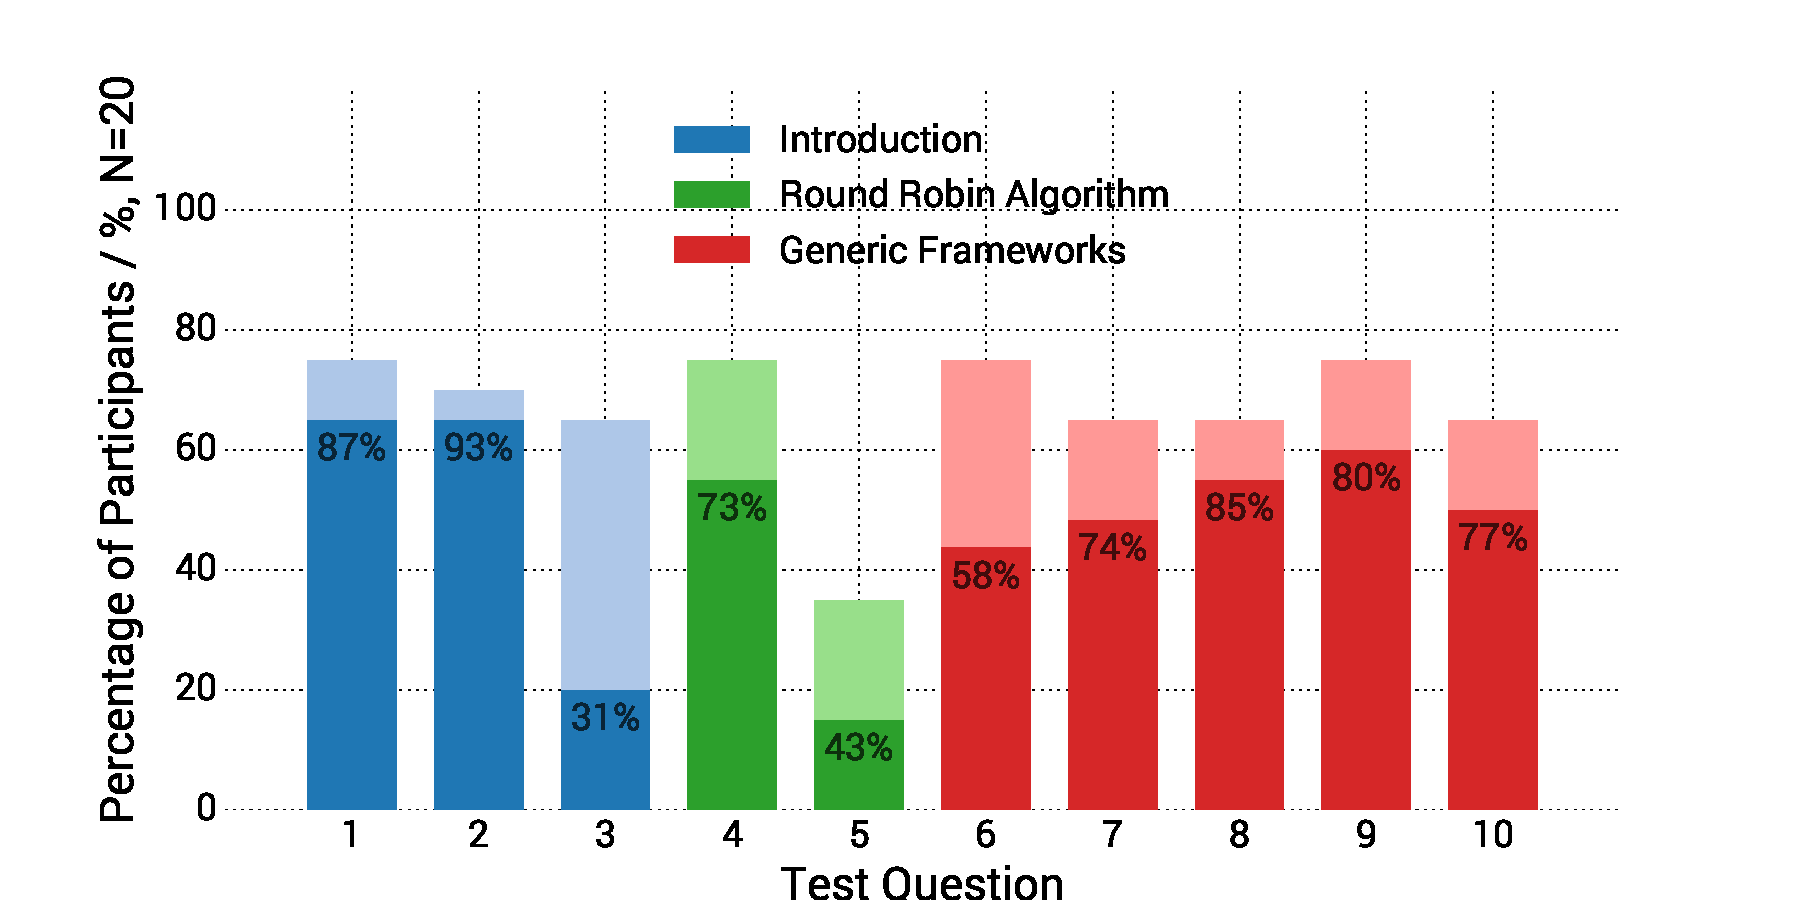
\includegraphics[width=\textwidth, trim=0 0 30 20, clip]{img/question_scores.pdf}
      \captionsetup{width=\textwidth, justification=centering}
      \caption{Attempts \& Answers to Test Questions}\label{fig:question-answers}
    \end{figure}

    The pale bars represent the number of participants who attempted
    each question, whilst the darker bars represent the average score
    achieved by all participants. The numbers in each bar represent
    the score achieved by those who attempted that question. Questions
    are color-coded by the lesson they are meant to assess.

    Most questions presented the user with 4 possible answers and
    allowed them to select only one. Questions 6 \& 7 allow multiple
    choices, but users are penalised for incorrect answers. The
    expected score obtained by random guessing is therefore
    approximately 25\%, or 1-in-4.

    During the in-person evaluations, some participants noted that
    they were confused by the submission button - they had expected it
    to submit only one question, when in fact it submitted the whole
    test. This could explain why all questions have an attempt rate
    below 80\%, the missing 20\% attributed to those who accidentally
    submitted the whole test.

    In addition, participants noted that questions 3 and 5 were
    misleading: the answer to question 3 appeared to be displayed in
    the accompanying diagram, so many participants did not realise
    they were required to perform a calculation and thus answered
    incorrectly. In addition, many participants felt that question 5
    was not covered by the lesson's content.

    Disregarding those two factors, the results are very
    positive. More than 85\% of participants understood the basic
    content, with only a slight drop in score as the complexity of the
    content increases. This implies that the application does, in
    fact, effectively teach the course content.

    Of course, these results are only an indication. It is highly
    possible that only academically-gifted participants took the
    test or that the questions covered content with which they were
    already familiar. However, the results are well above the expected
    average and optimistically show that the system achieved its goal.

    \subsection{User Opinion}

    In the feedback survey users were asked a number of
    \gls{likertscale} questions, rating their opinion on a scale from
    ``Strongly Agree'' to ``Strongly Disagree''. A response was
    mandatory for those who used each aspect of the system; the number
    of respondents can be found in the figure captions.

    Figures \ref{fig:opinion-simulator} \& \ref{fig:opinion-lessons}
    show the response to each item. The size of the ``Strongly Agree''
    and ``Strongly Disagree'' bars are doubled to visualise the
    weighted response to each item; the scores on the right-hand side
    show the actual average (5 being the most positive, 0 being the
    least).

    \begin{figure}[!hb]
      \centering
      \captionsetup{width=\textwidth, justification=centering}
      \caption{Opinion of the Round-Robin Simulator, N=22}\label{fig:opinion-simulator}
      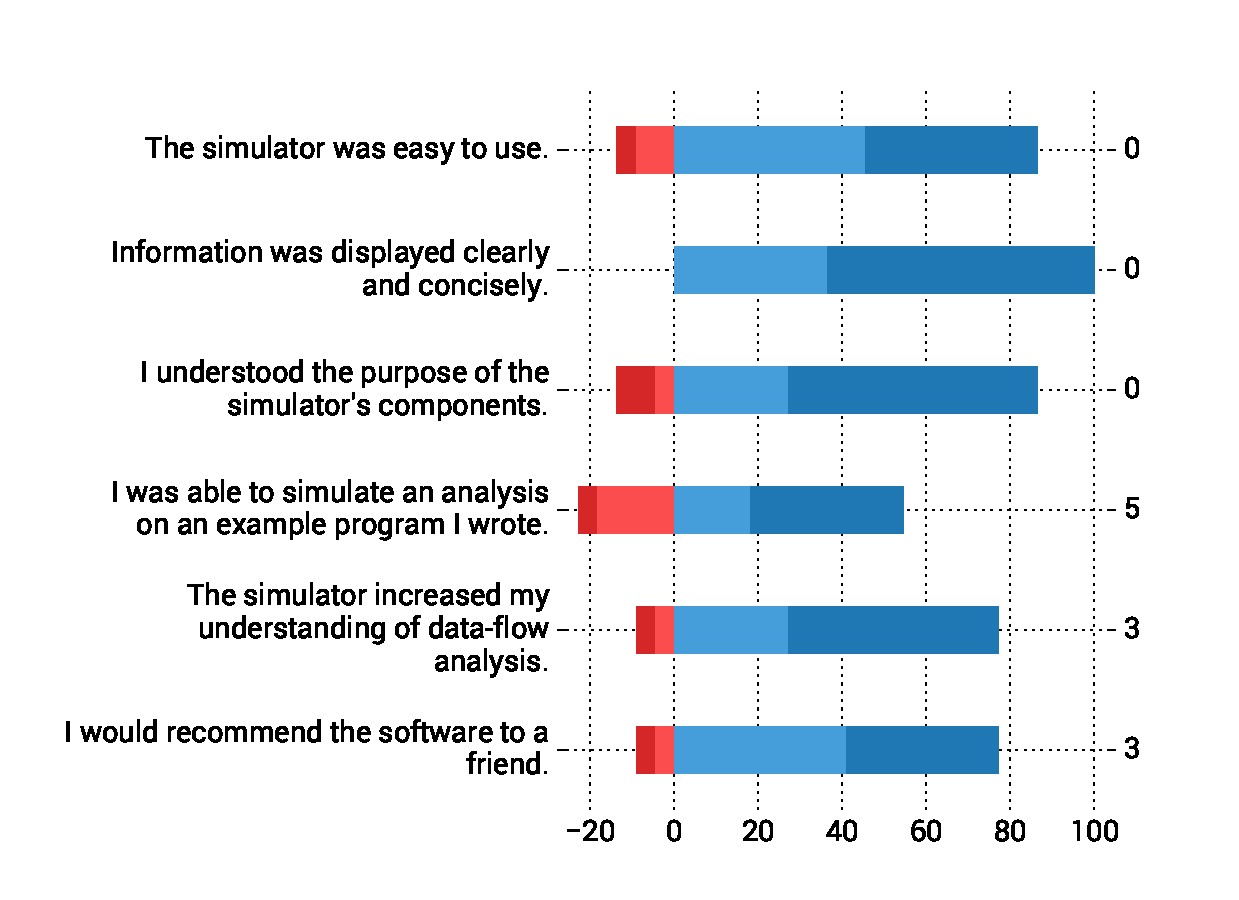
\includegraphics[width=\textwidth, trim=0 40 0 40, clip]{img/simulator_opinion.pdf}
    \end{figure}

    Reactions to the simulator were quite positive, with participants
    praising the way it displayed components of the analysis. Most
    users found the simulation easy to use, but there was some concern
    over the complexity of the interface and the content involved.

    One interesting point to note is that many users were unable to
    simulate an analysis on their own programs, or declined to respond
    to that item (perhaps for the same reason). Initially, the
    platform did not have any instruction as to how to write ILOC
    programs, so users were forced to rely on the examples in lessons
    and their own intuition for guidance. This oversight was corrected
    shortly after the evaluation period began by adding a help screen,
    which seems to have improved the response somewhat.

    \begin{figure}[!htb]
      \centering
      \captionsetup{width=\textwidth, justification=centering}
      \caption{Opinion of the Interactive Lessons, N=25}\label{fig:opinion-lessons}
      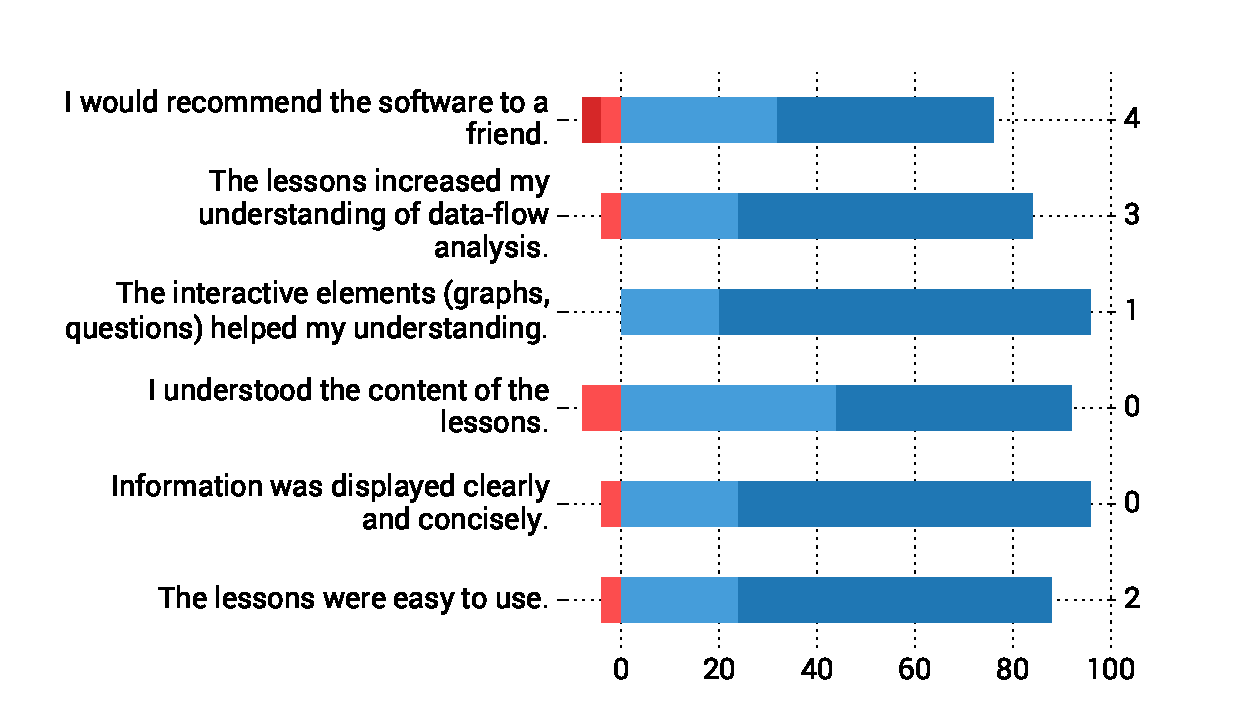
\includegraphics[width=\textwidth, trim=0 50 0 50, clip]{img/lesson_opinion.pdf}
    \end{figure}

    Opinion of the interactive tutorials was more positive -- most
    users agreed that the interface was easy to use and that the
    information was conveyed well. Users generally understood the
    content and all agreed that the interactive components helped
    increased their learning.

    Whilst the organisation of the content could use some improvement,
    it appears that overall opinion is that the system works
    well. Users were asked to select the methods of study they used
    most often, and how they would use the learning platform alongside
    those methods of study. The response to these questions is shown
    in figures \ref{fig:study-methods} \& \ref{fig:overall-opinion}.

    \begin{figure}[!b]
      \centering
      \begin{minipage}{.48\textwidth}
        \captionsetup{width=\textwidth, justification=centering}
        \caption{Overall User Opinion, N=27}\label{fig:opinion-overall}
        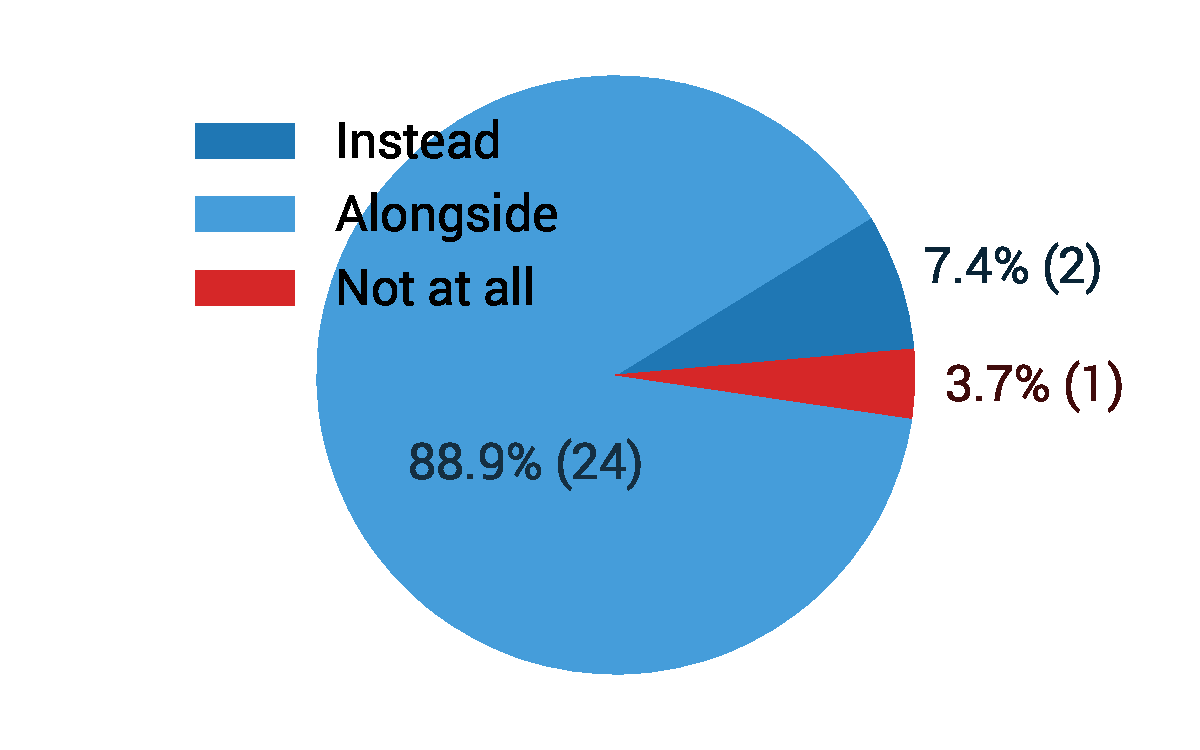
\includegraphics[width=\textwidth, trim=90 0 38 0, clip]{img/alternate_use_pie.pdf}
      \end{minipage}
      \quad
      \begin{minipage}{.33\textwidth}
        \captionsetup{width=\textwidth, justification=centering}
        \caption{Opinion on Future Use, N=27}\label{fig:future-use}
        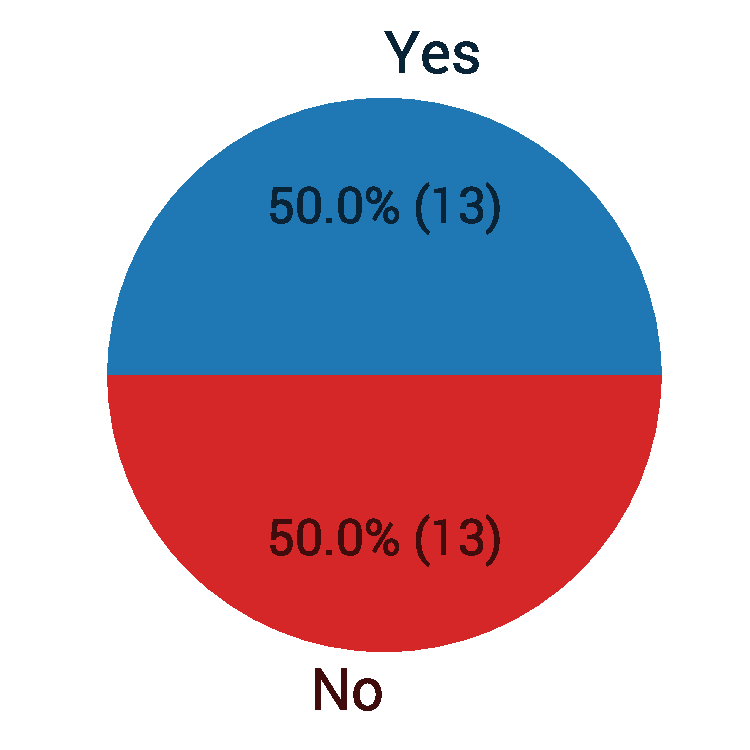
\includegraphics[width=\textwidth, trim=30 0 38 15, clip]{img/continued_use_pie.pdf}
      \end{minipage}
      \vspace{-1cm}
    \end{figure}

    The response to the first question was extremely positive -- only
    one person said that they would not use the platform to study over
    the other methods they chose. When asked if they planned to
    continue using the software after the evaluation period was over,
    exactly 50\% said that they would do so.
    
    Given the information about which methods participants use to
    study, this is hardly surprising -- the interactive tutorials are
    very similar to the most popular option (``Reading lecture slides
    / notes'') only with more active participation involved.

    \begin{figure}[!htb]
      \centering
      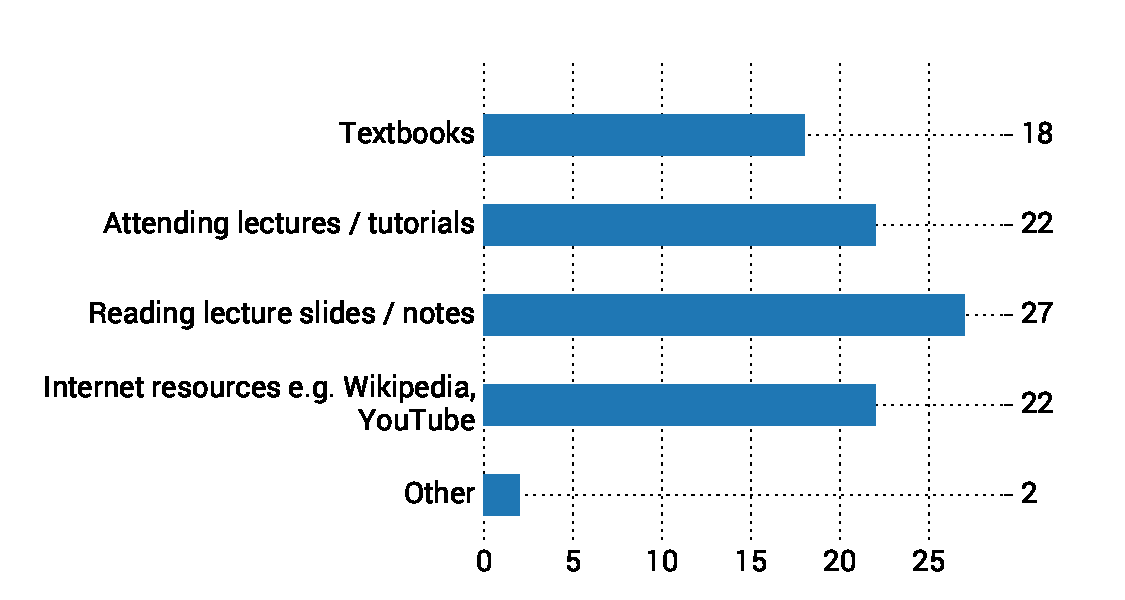
\includegraphics[width=\textwidth, trim=0 0 0 32, clip]{img/learning_methods.pdf}
      \captionsetup{width=\textwidth, justification=centering}
      \caption{Methods of Study, N=27}\label{fig:study-methods}
    \end{figure}

    \subsection{Written Feedback}
    
    Users were asked to provide written feedback both in the online
    invitations and throughout the survey, in order to gather insight
    into user opinion and potential improvements which could be
    made. A fair amount of the written feedback was incredibly
    positive; what follows is a selection of those comments:

    \begin{quote}
      \vspace{1mm}
      ``The lessons were quite interesting. I liked the concise and
      short amounts of information in each step - never felt
      overwhelmed.''
      \vspace{1mm}
    \end{quote}

    \begin{quote}
      \vspace{1mm}
      ``I wish the uni would use things like this for teaching - it's
      far easier to understand than parsing through lecture notes.''
      \vspace{1mm}
    \end{quote}

    \begin{quote}
      \vspace{1mm}
      ``This is superb! Thank you for this. I am just learning about
      dataflow analysis in my compilers course.''
      \vspace{1mm}
    \end{quote}

    \begin{quote}
      \vspace{1mm}
      ``... great job! I'm in my third year of PhD in compiler
      optimizations and found your tool really nice and illustratory
      ({\em thumbs-up emoji}).''
      \vspace{1mm}
    \end{quote}
    
    \begin{quote}
      \vspace{1mm}
      ``I like how upon giving a correct answer, it is still explained!
      When giving answers in first lesson, I was still not 100\% sure
      about them, so having them explained even when I was correct was
      nice.''
      \vspace{1mm}
    \end{quote}

    Of the negative feedback, most was constructive criticism. Users
    suggested a range of improvements to the site, primarily relating
    to the lessons and how they could be used to improve understanding
    of the simulation. Many users complained about the organisation of
    the main menu (\S\ref{sec:impl-menu}), due to the confusing order
    in which the menu items were laid out. Users also desired a
    summary of each lesson and the system as a whole; the menu does
    not really explain the purpose of the software, which put some
    users off exploring it further.

    Regarding the simulation, users were confused by the colour
    co-ordination and felt that it could have been improved upon. In
    addition, there was some concern about the lack of guidance. I had
    assumed that most people would complete the introductory lesson
    before playing with the simulator, but it appears that this was
    not the case -- or that perhaps it was difficult to relate the
    lesson content to simulator's components. One user in particular
    left the following comment:

    \begin{quote}
      ``Few bugs here and there but simulation is engaging... more could
      be done to link between decription and simulation.''
    \end{quote}

    The lessons also received some minor criticism. The most common
    opinion was that the interface lacked some basic features, such as
    an indicator of progress or the ability to navigate directly to
    each section of the lesson. The segmentation of content was met
    with a mixed response; some users complained that they had to
    click the ``Next'' button too many times whilst others appreciated
    that the information was split into bite-sized chunks.

    A small number of bugs were brought to my attention. Firstly, in
    Firefox browsers the navigation buttons do not always function as
    expected. Unfortunately this is due to an issue with the dagre-d3
    library, but it could be possible to patch it with further
    testing. Users also reported that the back button in their browser
    did not work. This was an oversight relating to the implementation
    of the {\tt View} system and could be fixed with some minor tweaks
    to the way pages are loaded.

    \section{Future Developments}
    
    Throughout this report suggestions have been made for potential
    improvements to the system, ranging from small usability changes
    such as adding progress indicators and navigation elements to
    overhauling the content in order to strengthen the link between
    the tutorials and the simulation. However, there has not yet been
    any discussion around long-term future developments or content to
    be covered.

    Participants in the survey who stated that they had used the
    simulator were asked to rank a list of potential future features
    in order from most to least important. The response to this
    question is shown in fig. \ref{fig:future-features}.

    \begin{figure}[!htb]
      \centering
      \captionsetup{width=\textwidth, justification=centering}
      \caption{Opinion on Future Simulator Improvements, N=22}\label{fig:future-features}
      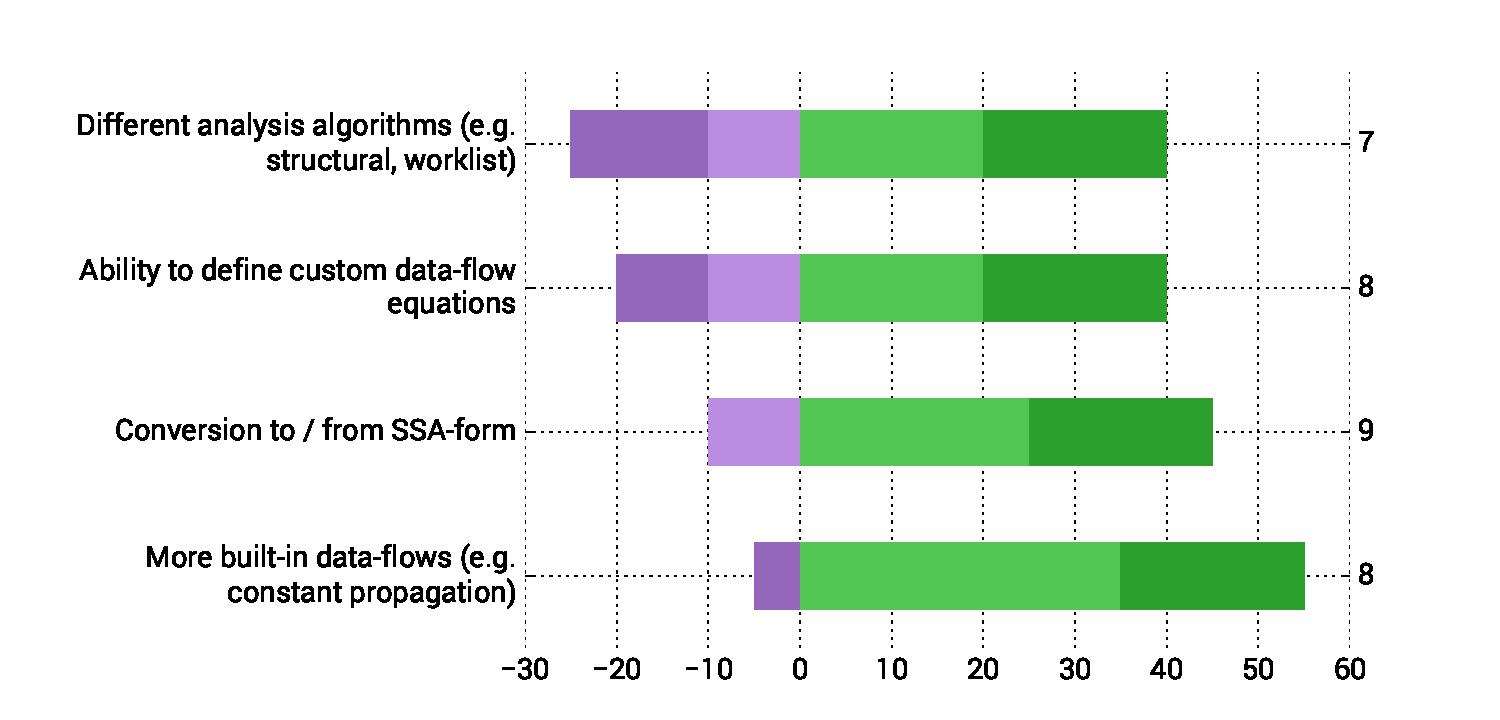
\includegraphics[width=\textwidth, trim=0 20 0 20, clip]{img/simulator_improvements.pdf}
    \end{figure}

    The choices listed were based on early discussions between myself
    and the project's supervisor, Hugh Leather. His original proposal
    for the project suggested a possible extension which would allow
    users to define their own data-flow frameworks and simulate an
    analysis using them. Although I chose to focus on other aspects of
    the system, this idea was one that I was keen to see realised if
    time permitted. Examining the responses it seems that focusing
    elsewhere was the right choice after all; users largely preferred
    that data-flows be written for them rather than by them, perhaps
    because they were not aware of how or why they would use this
    feature. Some of the written responses to the survey would agree
    -- participants wrote that although they had learned how to
    perform data-flow analysis, they did not know what they would use
    it for. To rectify this the content could be expanded to
    demonstrate the applications of the topic both in compilers and in
    other areas such as web security\cite{TaintedFlow}; maybe then
    users would find value in being able to write their own
    data-flows.

    The \gls{dataflow} framework system would need to be improved in
    order to add interesting new data-flows. Whilst it is certainly
    possible to add more \gls{bitvector}s, \gls{tuplevalued}s would
    need to be implemented to support \gls{dataflow}s such as constant
    propagation. This, in turn, would require an overhaul of the Hasse
    diagram visualisation to make it capable of displaying lattices
    for more complex \gls{dataflow}s.

    The second most popular improvement was conversion to and from
    SSA-form\footnote{Single Static Assignment (SSA) form is a
      transformation applied to control-flow graphs in which variables
      are copied and renamed so that every variable is defined only
      once.}. The lecture slides cover this topic quite heavily, but I
    decided against including it because its applications lie closer
    to performing compiler optimisations than to data-flow analysis
    itself. If the content were to be expanded, SSA-form would be one
    of the more simple features to include and would open the door to
    visualising optimising transformations such as code motion.

    Further down the line, the \gls{controlflowgraph} visualisation
    could be adapted to allow users to edit it directly. This improved
    visualisation would allow users to add, delete or edit nodes,
    making connections or removing them in order to explore how
    changing the \gls{cfg}'s structure or local information changes
    the problem's solution.

    Finally, the interactive tutorials have huge potential for
    enhancement. Currently, the main form of interaction is through
    multiple-choice questions. A more advanced system could allow
    users to write ILOC programs to solve problems, or if the custom
    \gls{dataflow} framework system were implemented users could be
    asked to write frameworks to solve a given \gls{dataflow}
    problem. The presentation of the content could be diversified
    using audio or video formats or automated demonstrations which
    control the user's mouse and keyboard.

    \section{Conclusion}
    The main objective of this project was to develop a learning
    platform for compiler data-flow analysis which provided a more
    interactive alternative to traditional teaching formats, and to
    demonstrate that such a system would be an effective tool for
    learning.

    The results collected throughout this evaluation are strong
    evidence that the project has achieved this goal. Reponse to the
    feedback survey was overwhelmingly positive; the visual and
    interactive elements received particularly high praise, as did the
    presentation of the material. Achievement of learning outcomes was
    well above average, users were kept engaged by the platform, and
    all but one participant stated that they would use the system
    alongside other methods of study.

    However, the end of a project is not only a time for praise. One
    must take the opportunity to reflect upon and learn from their
    performance. Much time was spent rectifying mistakes made early in
    development; whether caused by lack of experience or rushed
    decision-making, some forethought would not have gone
    amiss. Perhaps a different development process would have revealed
    these issues before they became significant problems, or more time
    should have been spent researching technlogies before diving into
    the implementation.    

    I hope to see others follow this project's example and extend the
    system I have developed or apply the concept to other topics. The
    system has proven that online platforms are a valuable and
    effective tool for learning, one which must be explored further in
    order to truly realise their potential.

    In closing, I would say this: applications like the one developed
    in this project are only the beginning. As more and more
    industries move online, it is only natural that teaching move with
    them. It is time for higher education institutions to diversify
    the ways in which they teach their students and make efforts to
    appeal to a range of learning styles. By developing their own
    tools such as this one or pooling their resources with an entity
    like Coursera, Universities can truly bring teaching into the
    digital age.
    
    

% use the following and \cite{} as above if you use BibTeX
% otherwise generate bibtem entries
\bibliographystyle{unsrtnat}
\bibliography{mybibfile}

\begin{appendices}

\chapter{Terminology}\label{appx:glossary}

\printglossaries

\chapter{Types of Data-Flow Analysis}\label{appx:analysistypes}

\bgroup
  \vspace{-5mm}
  \begin{tabular}{|l|p{5cm}|p{5cm}|}
    \hline
    {\bf Data-Flow}                         & {\bf Purpose}                                                                                              & {\bf Applications}                                                                              \\ \hline
    Dominators                              & Computes the set of nodes which \gls{dominate} the current node.                                           & Computing SSA form.                                                                             \\ \hline
    \Gls{reachingdefinition}s               & Computes the set of variable definitions which are available at points in the CFG.                         & Generating def-use chains for other analyses.                                                   \\ \hline
    \Gls{livenessanalysis}                  & Computes the set of variables whose current value will be used at a later point in the control flow graph. & Register allocation. Identifying useless store operations. Identifying uninitialised variables. \\ \hline
    \Gls{availableexpression}s              & Identifies expressions which been computed at a previous point in the CFG.                                 & Code motion.                                                                                    \\ \hline
    Anticipable Expressions                 & Computes expressions which will be computed along all paths leading from the current point.                & Code motion.                                                                                    \\ \hline
    Constant Propagation                    & Computes the set of variables which have a constant value based on previous assignments.                   & Constant propagation. Dead code elimination.                                                    \\ \hline
    Copy Propagation                        & Computes the set of variables whose values have been copied from another variable.                         & Dead code elimination. Code motion.                                                             \\ \hline
    Tainted Flow Analysis\cite{TaintedFlow} & Identifies unsafe operations which have been passed unsanitized {\em (tainted)} input as a parameter.      & Preventing security vulnerabilities such as SQL injection and XSS attacks.                      \\ \hline
  \end{tabular}
  \captionof{table}{Types of data-flow analysis.}
\egroup


\end{appendices}

\end{document}
